%!TEX TS-program = xelatex
%!TEX root = ../../maxwell2018thesis.tex

\chapter[Result Diversification and Stopping Behaviour]{Result Diversification and\\Stopping Behaviour}\label{chap:diversity}
In the previous chapter, we examined how varying the lengths of result summary snippets affected a searcher's stopping behaviours. Indeed, snippet text can provide information that may assist a searcher in satisfying their information need. Indeed, searchers may learn about a topic by issuing a variety of different queries to explore the topic space~\citep{kelly2015search_tasks}. Often, such topics are \emph{aspectual} in nature, where an underlying goal is to find out about the different facets, dimensions or aspects\footnote{We consider aspects in this chapter, defined as \emph{``roughly one of many possible answers to a question which the topic in effect poses''}~\citep{over1998trec}.} of the topic. An example of aspects within a topic is illustrated below, taken from TREC 2005 Robust Track, topic 347.

 % When developing an information need, searchers will often possess an incomplete mental model of the topic~\citep{belkin1980ask}. To address this deficiency in their mental model, a searcher will often issue a variety of different queries to explore the topic space~\citep{kelly2015search_tasks}. Often, such topics are \emph{aspectual} in nature, where an underlying goal is to find out about the different facets, dimensions or aspects\footnote{We consider aspects in this chapter, defined as `\emph{`roughly one of many possible answers to a question which the topic in effect poses''}~\citep{over1998trec}.} of the topic. An example of aspects within a topic is illustrated below, taken from TREC Robust Track~\citep{voorhees2006trec_robust} topic 347.

\begin{figure}[h]
    \centering
    \vspace{4mm}
    \resizebox{1\hsize}{!}{
    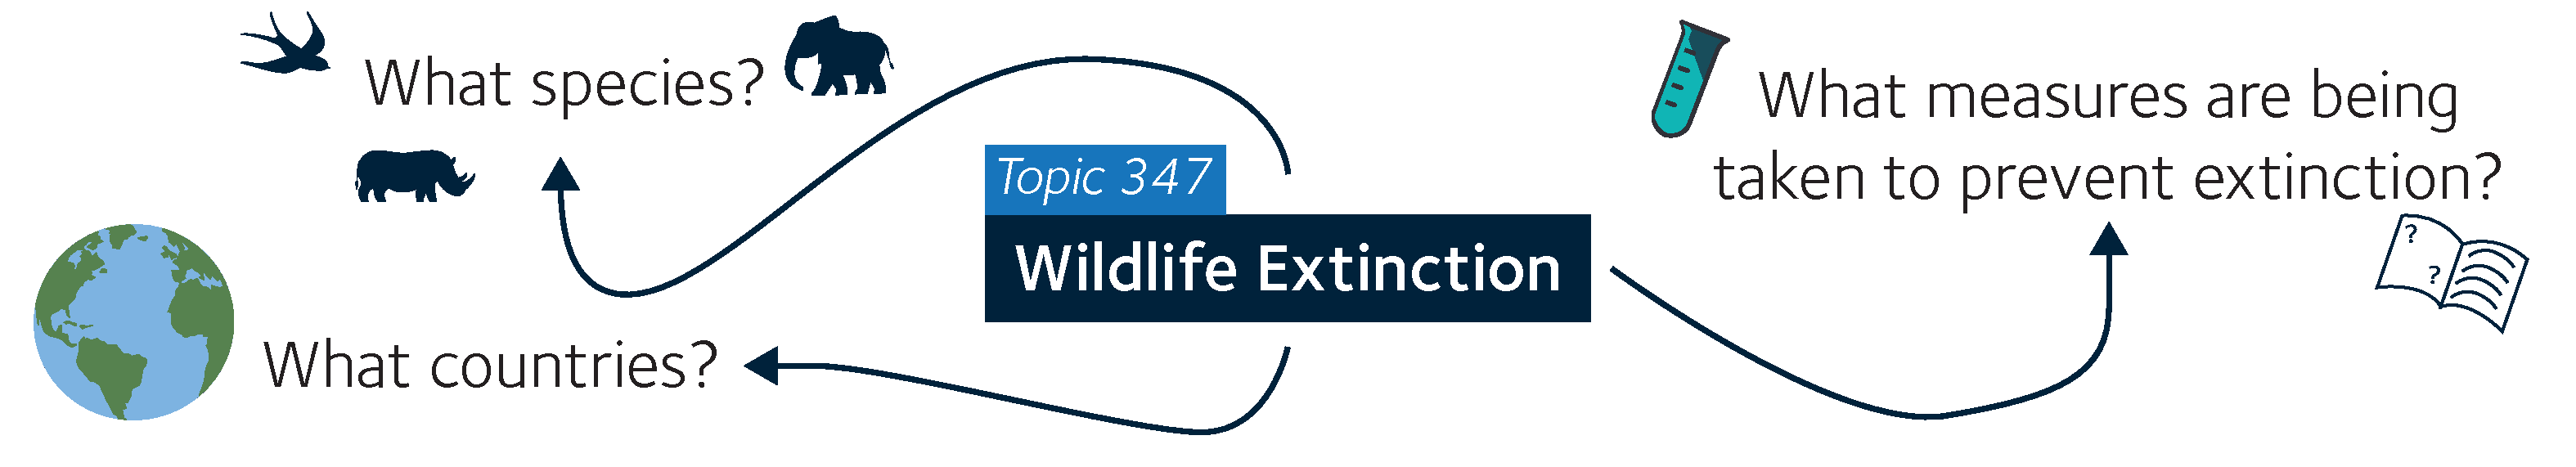
\includegraphics{figures/ch8-aspects_intro.pdf}}
    \label{fig:aspectsintro}
    \vspace{-5mm}
\end{figure}

While \emph{aspectual retrieval} has been heavily studied in the past (most prominently during the \emph{\gls{acr:trec} Interactive Tracks}~\citep{over2001trec}), there has been renewed interest in this type of search task. This is because it represents a novel context to explore the idea of \emph{``searching as learning''}~\citep{collins2017sal}. In this context, the goal of the system is to help the searcher learn about a topic~\citep{collins2017sal} -- and in doing so, the number of aspects the searcher finds provides an indication of how much they learned during the process~\citep{syed2017sal}. If the goal is to help searchers learn about a topic, then by returning results that are more diverse in nature and presenting a broader view of the topic, this \emph{should} assist searchers learn more about said topic. This reasoning suggests that employing \emph{diversification} will lead to an improved search and learning experience~\citep{syed2017sal}.

However, while there have been numerous diversification algorithms developed and proposed over the years\footnote{There are numerous examples of work on search result diversification, including measures such as \emph{Maximal Marginal Relevance (MMR)}~\citep{carbonell1998mmr}, and the \emph{xQuAD} framework~\citep{santos2010query_reformulations_diversification, santos2011intent}. Other studies in this area include works by~\cite{chen2006probabilistic_models} and~\cite{zhai2015subtopics}.}, the focus of the work reported in this chapter is on addressing the problem of intents, rather than how diversification affects complex search tasks, such as ad-hoc or aspectual retrieval. Thus, this chapter reports on:

\begin{itemize}
    \item{a \blueboxbold{user study}, exploring how diversifying results (or not) affects the search behaviour and performance of searchers when undertaking different search tasks, from one of ad-hoc or aspectual retrieval (Section~\ref{sec:diversity:users}); and}
    \item{a \blueboxbold{simulated analysis}, examining how the various stopping strategies proposed in Chapter~\ref{chap:strategies} perform under these tasks (Section~\ref{sec:diversity:simulated}).}
\end{itemize}

In particular, we use~\glsfirst{acr:ift}~\citep{pirolli1999ift} in this chapter -- outlined in Section~\ref{sec:stopping_background:theoretical:ift} on page~\pageref{sec:stopping_background:theoretical:ift} -- to derive a number of hypotheses, and thus ground our work. We begin this chapter however with a discussion of the prior work in the area, focusing upon aspectual retrieval, and a brief discussion of how~\gls{acr:ift} is used to provide us with a series of hypotheses about searcher behaviours across the different experimental conditions we trial.

\section{Background, Motivation and Hypotheses}\label{sec:diversity:background}
As discussed previously, a searcher will likely pose a varying number of queries (and~\glsplural{acr:serp}), and examine a number of documents (if any) before issuing a new query, or stopping their search altogether -- called \emph{session level stopping} (refer to Section~\ref{sec:csm:stopping} on page~\pageref{sec:csm:stopping}). The reasons for stopping at the session level are numerous, and can occur because searchers:

\begin{itemize}
    \item{they have simply found enough information~\citep{prabha2007enough, dostert2009satisficing, hassan2013beyond_clicks};}
    \item{have run out of time~\citep{zach2005enough_is_enough}; or}
    \item{were dissatisfied with what they found~\citep{kiseleva2015serp_fails}; or}
    \item{simply gave up their search~\citep{diriye2012abandonment}.}
\end{itemize}

Numerous works have shown that different factors influence search behaviours -- this is demonstrated in Chapter~\ref{chap:snippets}, for instance, which showed how varying the length of result summaries influences behaviours. However, of particular relevance to this chapter is how different \emph{search tasks} influence a searcher's behaviours~\citep{kelly2015search_tasks}.

\subsection{Aspectual Retrieval}
An interesting search task that has not received much attention in contemporary research is \emph{aspectual retrieval.} Aspectual retrieval is a type of search task that concerns the identification of different \emph{aspects} of a given topic. This task type differs from traditional ad-hoc retrieval in the sense that ad-hoc retrieval is concerned only with what constitutes a \emph{relevant} document to a given topic, rather than identifying relevant documents, and whether they are \emph{different} to what has been previously observed.

A relevant and different document will contain unseen aspects associated with the topic in question. With a graphical example provided at the beginning of this chapter, we now provide a further example to aid understanding. Consider the topic \emph{wildlife extinction} from the~\gls{acr:trec} 2005 Robust Track~\citep{voorhees2006trec_robust}. In an ad-hoc search task, if the searcher manages to find several documents concerning \texttt{'Pandas in China'}, these would all be considered relevant. However, for an aspectual retrieval task, where \emph{different} aspects must be found, the first document concerning \texttt{'Pandas in China'} is considered to be relevant/useful, and other aspects (in this case, the species of endangered animal) would need to be found, such as \texttt{'Sumatran Rhinos in Malaysia'}, \texttt{'Crested Ibis in Japan'}, etc.

Aspectual retrieval found significant traction in the \emph{\gls{acr:trec} Interactive Tracks}~\citep{over2001trec} from 1997-2002. The overarching goal of these tracks was to investigate searching, and an interactive task, by examining the processes involved, as well as the outcome~\citep{over2001trec}. Interaction was considered from the inaugural \emph{\gls{acr:trec}-1} in 1993~\citep{harman1993trec1}, where one group investigated interactive searching under the so-called \emph{interactive query mode} while undertaking an ad-hoc task. From \emph{\gls{acr:trec}-6} (1997) to \emph{\gls{acr:trec} 2002}, a substantial volume of research was directed towards the development of systems and search interfaces that:

\begin{itemize}
    \item{assisted searchers in exploring and retrieval various aspects of a topic, such as cluster-based and faceted interfaces that explicitly showed different aspects~\citep{mcdonald1998interactive, villa2009aspect_interface};}
    \item{provided tiles and stacks to organise documents~\citep{hearst1995tilebars, hearst1997texttiling, harper2006piling, iwata2012tilediversified}; and}
    \item{provided mechanisms to provide query suggestions that led to subjects following different search paths~\citep{kato2012query_suggestion, umemoto2016scentbar}.}
\end{itemize}

However, a disappointing conclusion from this initiative was that little difference was observed between such systems and the standard control systems (i.e. the traditional \emph{ten blue links}, as previously discussed in this thesis) -- both in terms of behaviour and performance~\citep{voorhees2005trec_book}.

As work shifted from aspectual retrieval to other areas, studies related to determining the intent of a searcher's query began to take hold, where the goal of this problem is to diversify the results retrieved with respect to the original query~\citep{rose2004understanding_user_goals}. Thus, this addresses the problem of \emph{ambiguity} for short, impoverished queries. This led to a series of diversification algorithms (and intent-aware evaluation measures), changing focus from the interface to the underlying algorithms and their evaluation measures. However, while there have been numerous studies investigating the effectiveness of diversification algorithms for the problem of query intents (e.g. one query, several possible interpretations), little work has looked at studying how such algorithms apply in the context of aspectual retrieval (e.g. one topic, many aspects). This is many due to the fact that most of these algorithms were developed \emph{after} the~\gls{acr:trec} Interactive Track concluded in 2002.

Recently however, a growing interest in new, more complex and exploratory search tasks has taken hold. This is true in the aforementioned context of \emph{``searching as learning''}~\citep{collins2017sal}.~\cite{syed2017sal} hypothesised that diversifying the results presented to searchers would improve their learning efficiency, and that this would be observed by a change in vocabulary expressed in their queries. The work reported in this chapter motivates our interest examining the effects of diversification when considering the task of aspectual retrieval, where a searcher needs to learn about different aspects of a topic. To ground our work, we now consider how search behaviours are likely to be changed by generating a series of hypotheses from~\gls{acr:ift}.

\subsection{Tasks and Information Foraging Theory}\label{sec:diversity:background:tasks}
To motivate our hypotheses for this chapter, we can draw upon~\gls{acr:ift}~\citep{pirolli1999ift}, and the \emph{patch model} in particular, to ground our research and provide insights into how search behaviours may change. The patch model, as detailed in Section~\ref{sec:stopping_background:theoretical:ift}, provides a mechanism for predicting how long foragers will stay in a patch before moving onwards to the next. Using the established approach discussed previously -- where moving between patches is akin to issuing a new query, while staying within a patch considered examining a~\gls{acr:serp} and linked documents -- we can then make a series of predictions as to how searchers will behave under different experimental conditions.

\begin{figure}[t!]
    \centering
    \resizebox{1\hsize}{!}{
    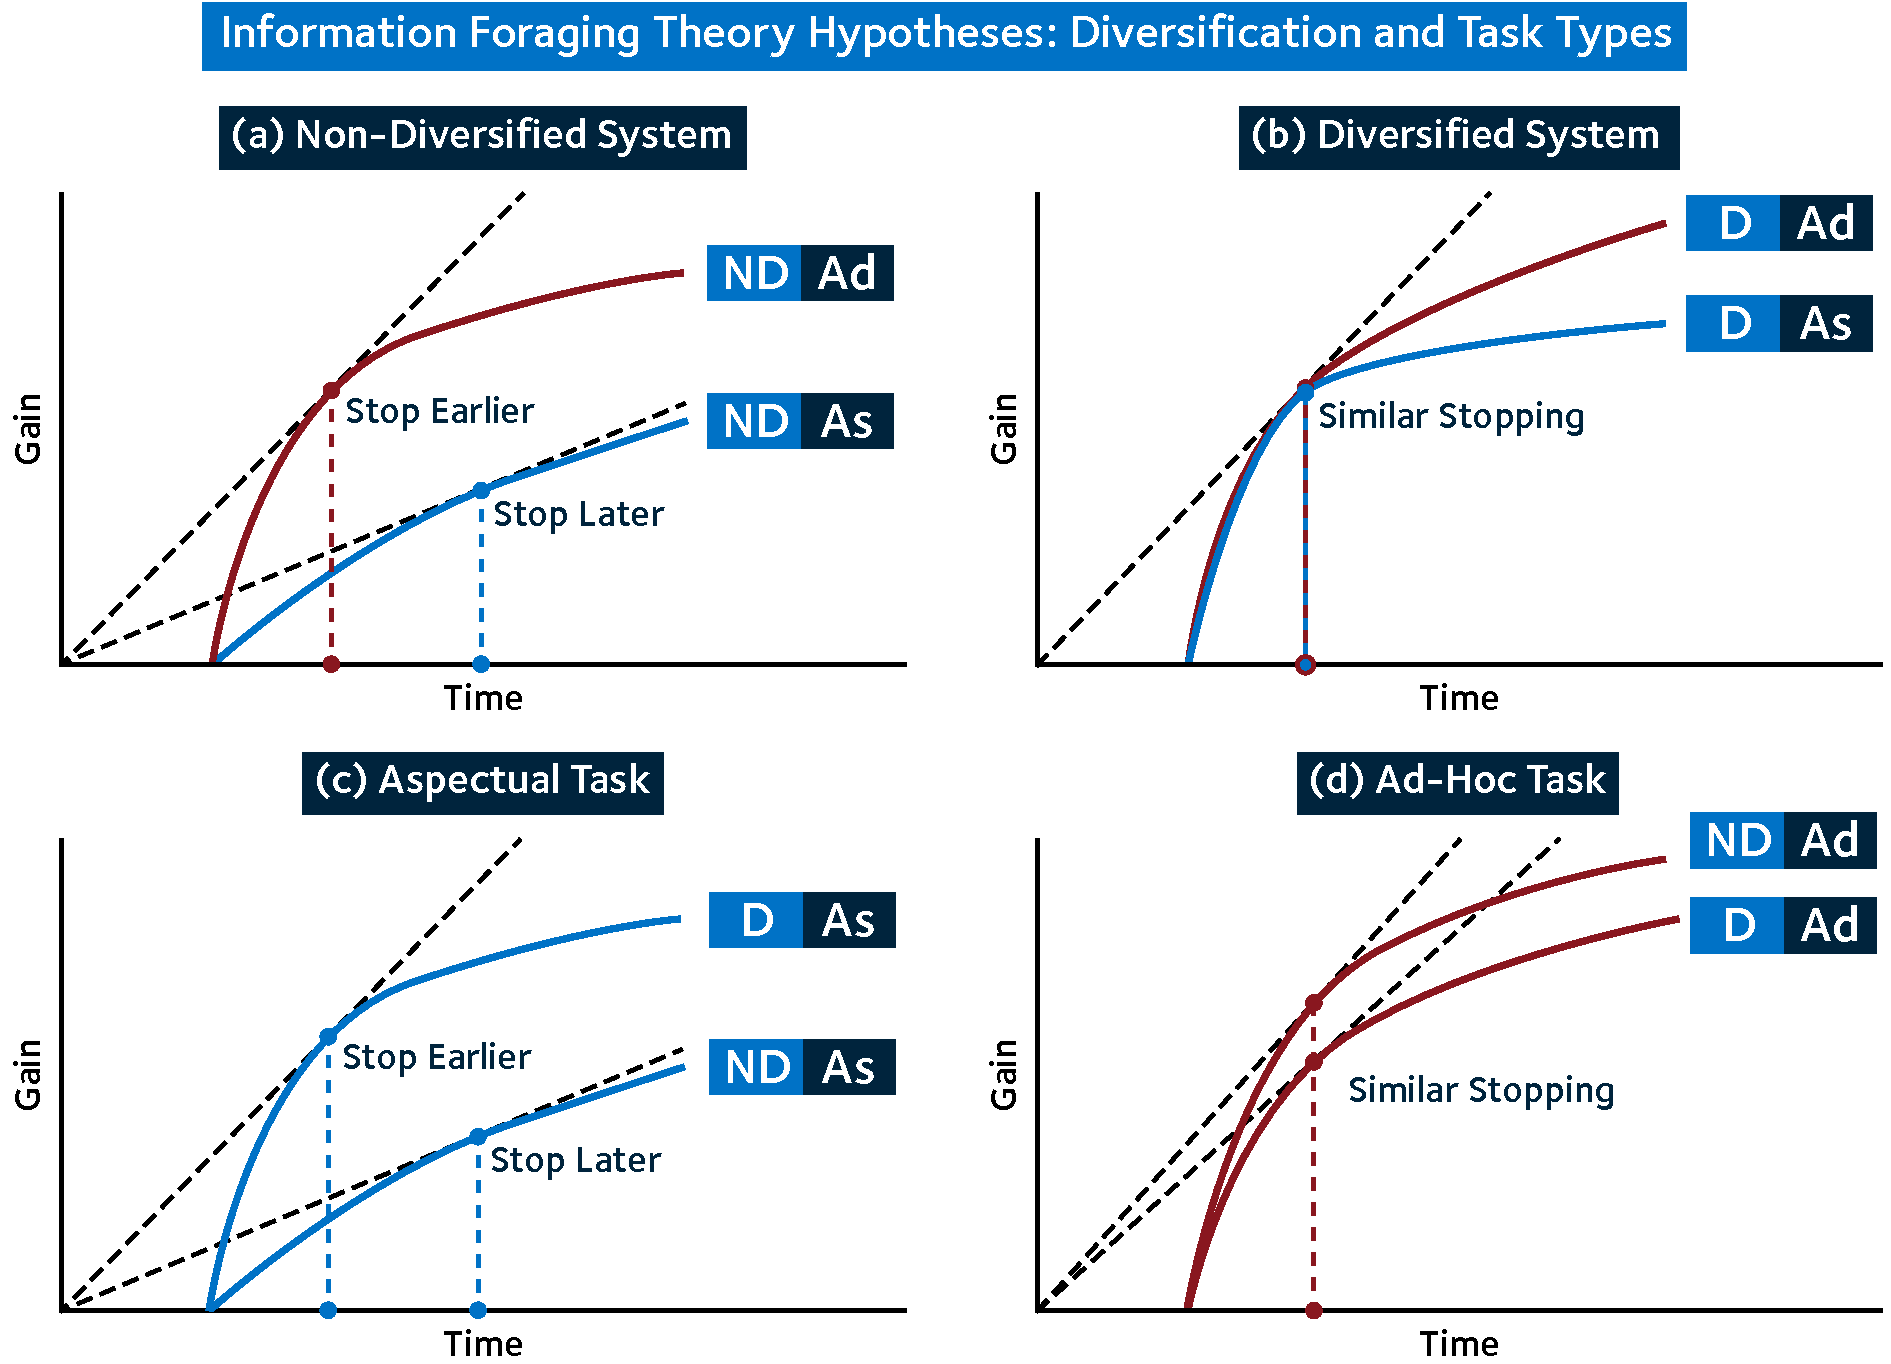
\includegraphics{figures/ch8-ift_theory_plots.pdf}}
    \caption[\gls{acr:ift} and diversification: hypothesis illustrations]{Graphical illustrations of the hypotheses motivated by~\gls{acr:ift}, with each plot showing how stopping behaviour is likely to be affected when using a system that \emph{(a)} diversifies results and \emph{(b)} doesn't, and over \emph{(c)} aspectual and \emph{(d)} ad-hoc tasks. Section~\ref{sec:diversity:users:method} enumerates the four different experimental conditions shown here, such as \dualbluebox{ND}{AD} for instance.}
    \label{fig:ift_theory}
\end{figure}

These predictions are graphically illustrated in the four plots shown in Figure~\ref{fig:ift_theory} -- over a diversified \blueboxbold{D} and non-diversified \blueboxbold{ND} system, with ad-hoc \darkblueboxbold{AD} and aspectual \darkblueboxbold{AS} retrieval tasks.\footnote{The system and task are combined together to produce a complete condition, such as \dualbluebox{ND}{AD} representing a non-diversified system, with an ad-hoc retrieval task.} Gain curves for each of the four conditions are shown. In top left plot~\ref{fig:ift_theory} \emph{(a)}, where a non-diversified system is being used, the gain curve for the ad-hoc retrieval task is higher. This is because any relevant document would contribute to the searcher's gain. Conversely, the gain curve is lower for the aspectual retrieval task. This is because similar relevant documents would not contribute to the overall level of gain experienced by the searcher.

From~\gls{acr:ift}, the optimal stopping point would be different between the two tasks. As we discussed in~\ref{sec:stopping_background:theoretical:ift}, we can graphically find this point by drawing a line from the origin to the tangent of the gain curve. Red and blue dots indicate the optimal stopping points for ad-hoc and aspectual retrieval, respectively.~\gls{acr:ift} therefore suggests that with a non-diversified system, searchers will examine more documents per query for aspectual retrieval tasks when compared to ad-hoc tasks.

Plot~\ref{fig:ift_theory} \emph{(b)} illustrates gain curves where a diversified system would be used, with gain curves for ad-hoc and aspectual retrieval being similar in nature. This is because the diversified should bring relevant but different documents closer to the top of the rankings earlier. In the case of ad-hoc retrieval, these relevant (even if different) documents would still contribute to the overall level of gain. For aspectual retrieval, relevant and different documents will also contribute to the overall level of gain experienced by the searchers -- up to the point where the documents become similar to previously examined material. Therefore,~\gls{acr:ift} appears to suggest that similar stopping behaviours would be observed when searchers use a diversified search system.

Plot~\ref{fig:ift_theory} \emph{(c)} shows the predicted stopping behaviour for the aspectual retrieval task, where we have plotted the aspectual gain curves from the system plots \emph{(a)} and \emph{(b).} Interestingly,~\gls{acr:ift} suggests that searchers will stop sooner when using the diversified system. As such, if searching for the same length of time, searchers would thus issue more queries. Finally, plot~\ref{fig:ift_theory} \emph{(d)} shows the predicted stopping behaviour for the ad-hoc retrieval task, where again we plot the curves from the respective systems in plots \emph{(a)} and \emph{(b).} Note that here, the gain curve for the diversified system may be a little lower as some irrelevant but different material may bubble up the rankings. However, as can be seen, we expect little difference overall between the two systems, and so we hypothesise that the two levels of gain (and searcher behaviours) will be approximately be the same. Consequently,~\gls{acr:ift} suggests that there will be little difference in terms of stopping behaviours between the two systems with ad-hoc retrieval tasks.

However, we found~\gls{acr:ift} to counter our intuitions as to how searchers would \emph{behave.} When using a standard, non-diversified retrieval system, our intuition suggests that since the aspectual retrieval task is rather exploratory, searchers are then more likely to issue more queries as they learn about the topic, and try to explore efforts made by different countries to protect different specifies, for example.~\cite{kelly2015search_tasks} for example showed that more complex search tasks required a greater number of queries. If a searcher submits a query that retrieves relevant material such as \texttt{'protecting Pandas in China'}, then one would expect them to only select one or two examples, rather than many more. In the case of ad-hoc topic retrieval, we would \emph{intuitively} expected that searchers would issue fewer queries and examine more documents. This is because they don't need to find multiple aspects. However, when using a diversified system, which attempts to promote different aspects of a given topic, we would \emph{intuitively} expect that the behaviour of searchers would change, such that when undertaking aspectual retrieval, they would issue fewer queries and examine a greater number of documents per query.

\subsubsection{Hypotheses}\label{sec:diversity:background:tasks:hypotheses}
From the plots and descriptions provided above, we can formulate a number of different hypotheses relating to the expected searcher behaviours under different contexts.

Under aspectual retrieval search tasks, using a diversified system will lead to:
\begin{itemize}
    \item{\darkblueboxbold{H1} fewer documents examined per query; and}
    \item{\darkblueboxbold{H2a} more queries issued; or}
    \item{\darkblueboxbold{H2b} a decrease in the task completion time.}
\end{itemize}

With ad-hoc retrieval tasks, diversification will lead to:
\begin{itemize}
    \item{\darkblueboxbold{H3} no difference in the number of documents examined; and}
    \item{\darkblueboxbold{H4} no difference in the number of queries issued.}
\end{itemize}

While the contradiction between~\gls{acr:ift} and our intuitions provides an ulterior hypothesis. In addition, given the findings demonstrated by~\cite{syed2017sal}, we also hypothesis that diversification will lead to a greater awareness of the topic, regardless of the task put forward, as more aspects will be encountered and found.

\section{Diversifying Search Results}\label{sec:diversity:users}
Following on from the motivation and experimental,~\gls{acr:ift}-based hypotheses outlined above, this section discusses the user study that was undertaken in order to examine the aforementioned hypotheses. As per our general user study methodology discussed previously in Section~\ref{sec:methodology:user}, we conducted a within-subjects experiment, with the specific details for this study discussed in Section~\ref{sec:diversity:users:method} below.

The primary research question for this user study is as follows.

\begin{itemize}
    \item{\darkblueboxbold{RQ} How does diversification affect the search performance and behaviour when searchers under ad-hoc and aspectual retrieval tasks?}
\end{itemize}

This research question is addressed in tandem with the hypotheses put forward above in Section~\ref{sec:diversity:background:tasks:hypotheses}. Below, we now discuss the specific details for this user study, before discussing the results, with an emphasis on stopping behaviours, and whether or not the empirical evidence supports our hypotheses.

\subsection{Methodology}\label{sec:diversity:users:method}
As discussed above, this section outlines the specific details of this user study, and is to be considered in conjunction with the general user study methodology we employ, outlined in Section~\ref{sec:methodology:user}. The same basic retrieval system employing BM25, document corpus and topics were used as previously discussed.

The within-subjects study considers two key factors: the \emph{system} and the \emph{task.} For the system factor, our baseline control system was based upon BM25 (i.e. no diversification), and a diversified system. The details of our diversification approach are discussed in Section~\ref{sec:diversity:users:diversifying}. For the task factor, we used the standard ad-hoc retrieval task, and compared this against the aspectual retrieval task. This resulted in a $2x2$ factorial design. Each subject who took part in this study therefore completed four different search tasks, one in each of the four conditions (as we enumerate below). Each of the conditions were assigned using a Latin square rotation to minimise any ordering effects. The conditions listed below are also used in Section~\ref{sec:diversity:background:tasks} when explaining the plots supporting our hypotheses.

The first two conditions consider a non-diversified retrieval system \blueboxbold{ND} (i.e. BM25, our baseline).

\begin{itemize}
    \item{\dualbluebox{ND}{AS} A non-diversified system, with an aspectual retrieval task.}
    \item{\dualbluebox{ND}{AD} A non-diversified system, with an ad-hoc retrieval task.}
\end{itemize}

Our second set of conditions therefore consider a diversified system \blueboxbold{D}, using BM25 as a baseline and an additional diversifying component, as we discuss later in Section~\ref{sec:diversity:users:diversifying}.

\begin{itemize}
    \item{\dualbluebox{D}{AS} A diversified system, with an aspectual retrieval task.}
    \item{\dualbluebox{D}{AD} A diversified system, with an ad-hoc retrieval task.}
\end{itemize}

With non-diversifying and diversifying systems, we developed different sets of branding for each system, each with their own distinct colour scheme, name and logo. This was to assist searchers in differentiating between the two. First, in terms of branding, we created two fictional search engine names:

\begin{itemize}
    \item{\hula, representing the non-diversified \blueboxbold{ND} system; and}
    \item{\yoyo, representing the diversified \blueboxbold{D} system.}
\end{itemize}

\begin{figure}[t!]
    \centering
    \resizebox{1\hsize}{!}{
    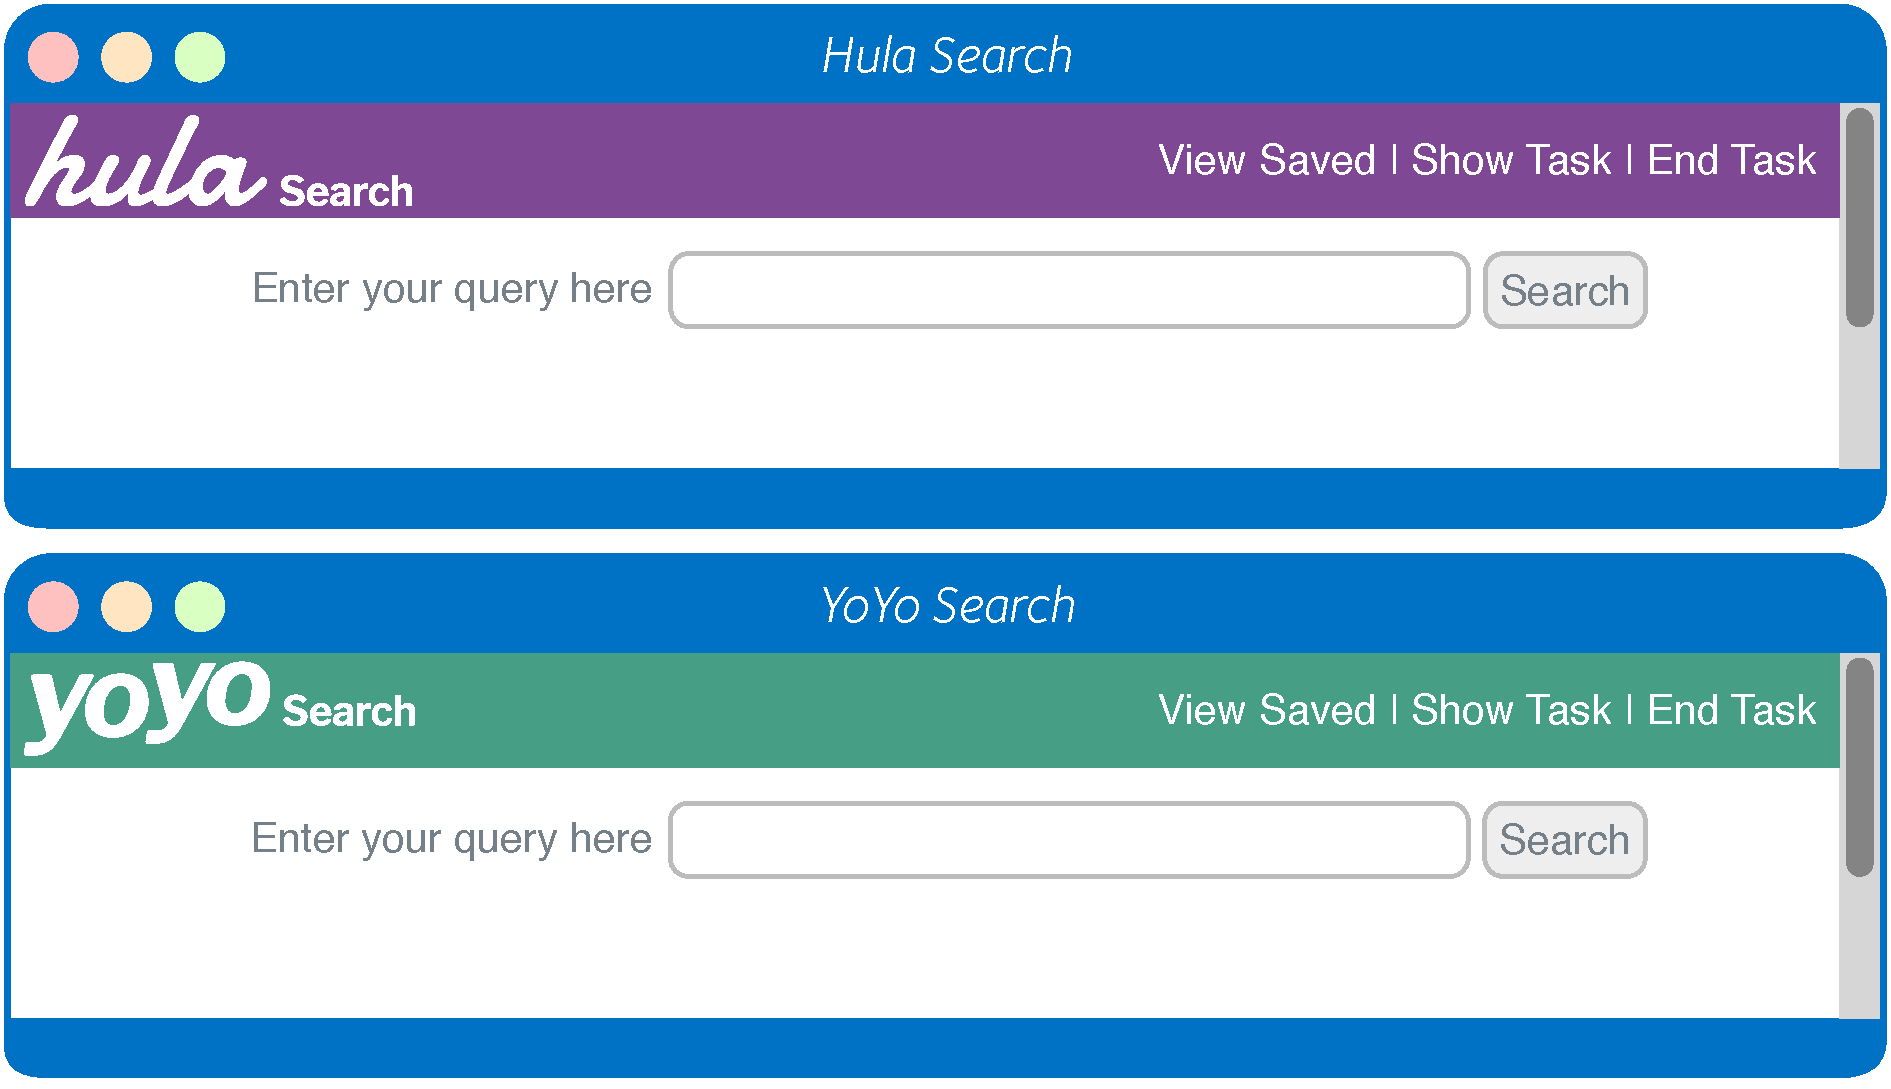
\includegraphics{figures/ch8-interface_headers.pdf}}
    \caption[Diversity user study interface mockups]{Mockups of the two names and colour schemes used to differentiate between the two experimental systems used in this user study. \hula~and \yoyo~represented the non-diversified and diversified systems respectively. Refer to Section~\ref{sec:diversity:users:method} for more information.}
    \label{fig:interface_headers}
\end{figure}

These names were chosen as they were not associated with any major search engine (to the best of our knowledge), nor did they imply that one of the systems performed better than the other. Colour schemes were chosen to provide the greatest different in visual appearance to those with colourblindness.\footnote{Two of the more common variants of colourblindness, \emph{protanopia} and \emph{deuteranopia,} were both considered.} This was to ensure that subjects could later on indicate what one of the two systems that they preferred, for example. Note that only the colour schemes and logos varied -- the same basic interface layout as previously discussed in Section~\ref{sec:methodology:user:interface} was employed. Figure~\ref{fig:interface_headers} demonstrates the two different colour schemes and logos for the two systems.

For the practice task, it should be noted that the standard, blue colour scheme as shown in Figure~\ref{fig:interfaces} on page~\pageref{fig:interfaces} was used. This is the same colour scheme as used in the user study reported in Chapter~\ref{chap:snippets}. A standard \texttt{News Search System Study} title was also used in place of any logos. This decision was taken to remove any impact that incorporating an individual system's colour scheme in the practice task would have on searcher behaviour or perceptions. All subjects used the \dualbluebox{ND}{AS} system and task for the practice task.

\subsubsection{Search Tasks}\label{sec:diversity:users:method:tasks}
As we discussed in Section~\ref{sec:methodology:user:flow}, subjects were grounded by instructing them to imagine that they were newspaper reports. As such, they were required to gather documents to write stories about the four topics they searched for. Given each topic, each subject was then further instructed for this study to focus on a different criterion.

\begin{itemize}
    \item{For \blueboxbold{ad-hoc retrieval} tasks, subjects were simply instructed to find documents that were \emph{relevant} to the topic provided.}
    \item{For \blueboxbold{aspectual retrieval} tasks, subjects were instructed not only to find documents that were relevant, but also discussed \emph{different} aspects of the provided topic.}
\end{itemize}

For example, take the \emph{Airport Security} topic (refer to Section~\ref{sec:methodology:collection:topics}). Under an ad-hoc retrieval task, subjects were required to learn about the efforts taken by international airports to better screen passengers and their carry-on luggage. For aspectual retrieval tasks, subjects were also asked to find relevant documents that are different, mentioning \emph{new airports.} Thus, subjects were explicitly instructed to find a number of examples from different airports, as opposed to a similar or the same example based in the same airport multiple times.

\blueboxheader{Task Goal}
Instead of imposing a time limit as per the user study reported previously in Chapter~\ref{chap:snippets}, we instead instructed subjects to find and save at least four useful documents -- with useful denoted as being relevant, or relevant and different, depending upon the given task. Refer to the following section for details on the reasons behind selecting this value. As such, subjects had the liberty to end the search task when they chose to do so by selecting the \texttt{End Task} option at the top right of the search interface -- refer to Figure~\ref{fig:interface_headers} for examples of this. This is in direct contrast to the user study reported in Chapter~\ref{chap:snippets}, where subjects were required to search for a full ten minutes before being directed to the next step in the experimental process.

\subsubsection{Crowdsourced Subjects and Controls}
Subjects undertaking the user study were informed that from a small-scale pilot study, it would take approximately 7-10 minutes of their time to find at least four useful documents per task. Combining everything together, this meant that the entire experiment would take approximately 40-50 minutes of their time. Since we did not impose any time constrains on how long subjects searched for, we instead established accuracy based control. We informed subjects that their accuracy in identifying useful material would be examined, and that they were required to find four useful documents with at least $50\%$ accuracy (based upon~\gls{acr:trec} relevance judgements as the gold standard). Using data from the prior user study reported in Chapter~\ref{chap:snippets}, the accuracy of those subjects was between $25\%$ and $40\%$ on average, depending upon the topic. While we stipulated a higher accuracy, this was to motivate subjects to work diligently.

In all, a total of $64$ subjects performed the the experiments that complied with the~\gls{acr:mturk} recruiting constraints we imposed, as we outlined in Section~\ref{sec:methodology:user:crowdsourcing} on page~\pageref{sec:methodology:user:crowdsourcing}. However, a total of $13$ were omitted from this figure because they either:

\begin{itemize}
    \item{failed to complete all the search tasks (a total of five subjects were removed);}
    \item{failed to mark at least four documents (two subjects); or}
    \item{spent less than two minutes per task, and failed to retrieve any relevant documents (six subjects).}
\end{itemize}

Of the $51$ subjects who successfully completed the experiment, $26$ females and $25$ males participated. The average age of the subjects was $38.66$ years ($min=20$; $max=71$; $stdev=11.43$). In addition to these basic demographics, a total of $22$ subjects reported possessing a bachelor's degree or higher, with the remaining $29$ possessing an associate's degree or lower. All subjects bar one expressed a preference to \emph{Google} as their everyday search engine of choice. All subjects indicated that they conducted many searches for information via a search engine per week. Nearly three quarters of the subjects ($38$) reported using a mouse of the experiment, with the remaining $13$ using a form of trackpad.

\subsubsection{Extracting Aspects}\label{sec:diversity:users:method:aspects}
For each topic, we used corresponding~\gls{acr:trec} QRELs from the 2005 Robust Track~\citep{voorhees2006trec_robust}. However, to assess how many aspects were retrieved by subjects, we needed to commission additional labels as existing labels were not available for all the selected topics. First, for each topic, we examined the topic descriptions to identify what dimensions could be considered aspects of the topic. We noted that for each topic, there was at least two ways this could be achieved: \emph{entity-} or \emph{narrative-based}. For example, a useful document the topic \emph{Curbing Population Growth} could either state the country taking measures (entity-based), or a description of the actual measure used to reduce population growth (narrative-based).

\begin{table}[t!]
    \caption[Entity- and narrative-based topic aspects]{A list of the different entity- and narrative-based approaches trialled during the aspect extraction process. As discussed in Section~\ref{sec:diversity:users:method:aspects}, the entity-based approach was carried forward for this study with a higher agreement rate between assessors.}
    \label{tbl:entities_across_topics}
    \renewcommand{\arraystretch}{1.8}
    \begin{center}
    \begin{tabulary}{\textwidth}{L{3.75cm}@{\CS}D{3.75cm}@{\CS}D{7.75cm}@{\CS}}
    
    & \lbluecell\textbf{Entity} & \lbluecell\textbf{Narrative}\\
    
    \RS\lbluecell\textbf{Airport Security} & \cell Airports & \cell Security measures taken \\
    \RS\lbluecell\textbf{Wildlife Extinction} & \cell Species & \cell Protection and conservation measures \\
    \RS\lbluecell\textbf{Piracy} & \cell Vessels boarded & \cell Acts of piracy \\
    \RS\lbluecell\textbf{Tropical Storms} & \cell Storms & \cell Lives lost, destruction caused \\
    \RS\lbluecell\textbf{Curb. Pop. Growth} & \cell Countries & \cell Population control methods \\
    
\end{tabulary}
\end{center}
\end{table}

For this study, it was decided that we should focus on entity-based aspects. This decision was taken as \emph{different narratives} were subject to greater interpretation that \emph{different entities} -- it is easier to identify from a document that China, for example, is the country being discussed, rather than the measures the country took -- and their effects. For each~\gls{acr:trec} relevant document across the five topics considered, the author and his supervisor manually extracted the different aspects for each, with much higher agreement ($95\%$ vs. $67\%$) between the author and his supervisor across the entity-based aspects. Both the entity and narrative based approaches for each of the five topics are shown in Table~\ref{tbl:entities_across_topics}.

To complement Table~\ref{tbl:entities_across_topics}, we also list below a number of different example entity-based aspects that were extracted for each of the five topics. The number provided with the topic title denotes the number of individual aspects that were extracted for said topic.

\begin{itemize}
    \item{\blueboxbold{Airport Security (14 unique aspects)} Considering different \emph{airports} in which additional security measures were taken, examples include \emph{John F. Kennedy International Airport, Boston Logan International Airport,} or \emph{Leonardo da Vinci International Airport.}}
    \item{\blueboxbold{Wildlife Extinction (168 unique aspects)} Considering different \emph{species of endangered animals} under protection by states, such as the \emph{golden monkey, Javan Rhino,} or \emph{Manchurian tiger.}}
    \item{\blueboxbold{Piracy (18 unique aspects)} Considers different \emph{vessels} that were either boarded or hijacked, such as the \emph{Petro Ranger, Achille Lauro} or \emph{Global Mars.}}
    \item{\blueboxbold{Tropical Storms (43 unique aspects)} Considers different \emph{tropical storms} where individuals were killed, and/or there was major damage, such as \emph{Hurricane Mitch, Typhoon Linda} or \emph{Tropical Storm Frances.}}
    \item{\blueboxbold{Curbing Population Growth (26 unique aspects)} Considers different \emph{countries} where population control methods were employed, such as \emph{China, India} or \emph{Zimbabwe.}}
\end{itemize}

Each of the unique aspects were assigned an identifying number, and stored in the~\gls{acr:trec} diversity format. By storing the aspects in this format, this then permitted us to use the \texttt{ndeval} evaluation tool\footnote{The \texttt{ndeval} source code can be acquired from the~\gls{acr:trec} website at \url{https://trec.nist.gov/data/web/10/ndeval.c}. \urlaccessed{2018-06-24}}, which was in turn used to compute a number of measures related to aspectual retrieval. This process is illustrated in Figure~\ref{fig:entity_ids} (with the wildlife extinction topic used as an example).

\begin{figure}[t!]
    \centering
    \resizebox{1\hsize}{!}{
    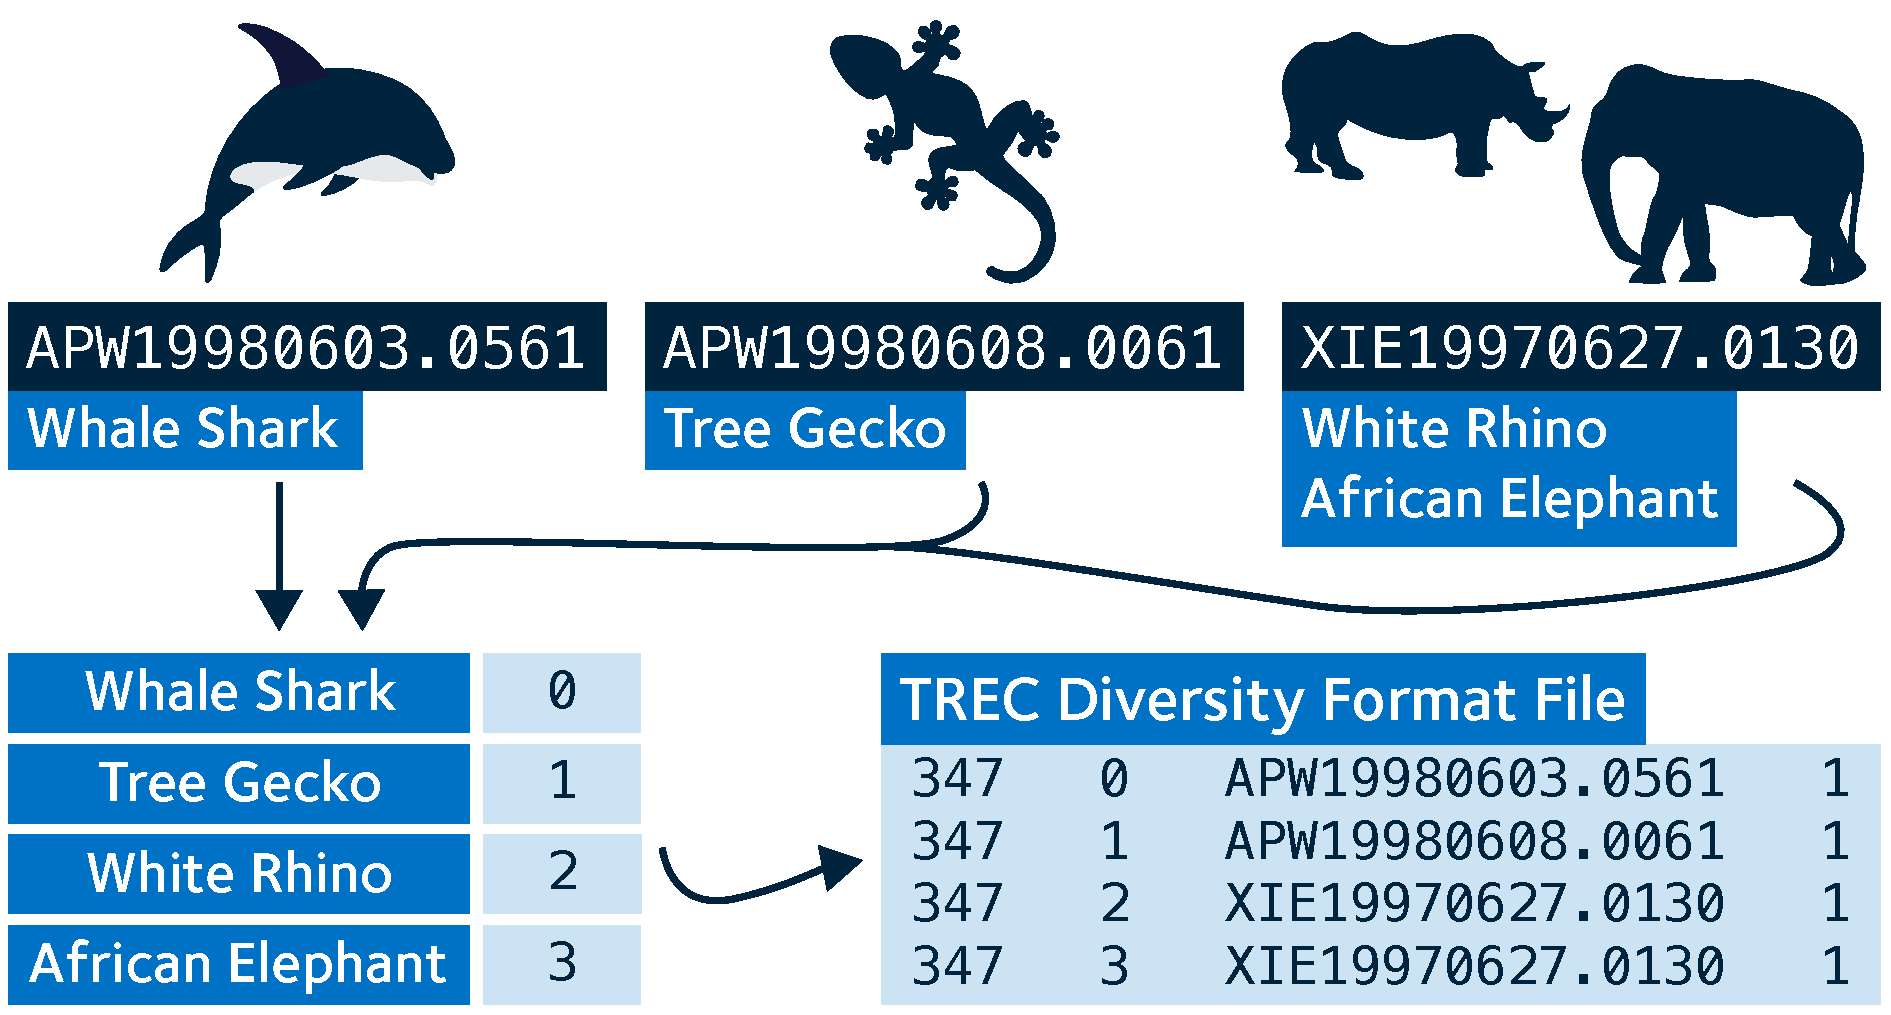
\includegraphics{figures/ch8-entity_ids.pdf}}
    \caption[Entity-based aspects example]{An example of documents, each with one or more entity-based aspects discussed within them. From these identified aspects, we can then provide a unique identifier for each aspect per topic, before creating a~\gls{acr:trec} diversity format file to be used in evaluation applications such as \texttt{ndeval}, allowing us to compute many diversity-based measures.}
    \label{fig:entity_ids}
\end{figure}

\subsubsection{Additional Performance Measures}\label{sec:diversity:users:measures}
In conjunction with the standard performance measures that we discussed back in Section~\ref{sec:methodology:extracting:performance} on page~\pageref{sec:methodology:extracting:performance}, we also include for this chapter two additional measures that consider aspectual search tasks. While traditional measures consider what documents are relevant, these additional measures allow us to determine \emph{why} said documents are relevant (i.e. what aspects each document covers).

The first measure we consider is \emph{aspectual recall (AR).} As part of the TREC-6 campaign,~\cite{over1998trec} defined aspectual recall as:

\begin{quote}
    \emph{``...the fraction of the submitted documents which contain one or more aspects.''}
    \attrib{\cite{over2001trec}}
\end{quote}

\begin{wrapfigure}[3]{r}{0.45\textwidth}
    \begin{center}
    \vspace*{-10mm}
    
\includegraphics[width=1\textwidth]{figures/ch8-aspectual_recall.pdf}
    \end{center}
    \label{fig:aspectual_recall}
\end{wrapfigure}

Given a ranking, aspectual recall can be therefore computed by summing the number of \emph{unseen aspects} regarding a given topic up to a given ranking, $k$, and dividing by the rank. This is in contrast to more simplistic relevance measures that consider only the~\gls{acr:trec} relevance judgement score for a document and topic combination. An example is provided above: given three documents, with three, one and zero new aspects to a topic, the aspectual recall at rank 3 is therefore $(3+1+0)/3 = 1.33$.

In addition to aspectual recall, \emph{aspectual precision} was also defined by~\cite{over2001trec} as \emph{``the fraction of total aspects...for the topic that are covered by the submitted documents.''} Given this definition, it was argued by~\cite{sanderson2010test} that aspectual precision appears to be the same as aspectual recall, and thus we do not report aspectual precision in this chapter.

The second measure that considers the diversity of the results returned is $\alpha DCG$. A~\glsfirst{acr:cg}-based approach, we discuss~\gls{acr:cg} basics in Section~\ref{sec:ir_background:evaluation:system:cg}. An extension of~\glsfirst{acr:dcg}~\citep{jarvelin2002cg}, $\alpha DCG$ employs a position-based user model~\citep{clarke2008adcg}. The measure takes into account the position at which a document is ranked along with the aspects contained in the documents. $\alpha DCG$ ranks by rewarding newly-found aspects, and penalising redundant aspects geometrically, discounting all rewards with a discounting rank function. As the name of the measure might imply, $\alpha$ is a tuneable parameter, controlling the severity of redundancy penalisation. As used in prior~\gls{acr:trec} experimentation, we used $\alpha=0.5$ for all reporting of $\alpha DCG$ in this chapter.
% Based on "Analysis of Various Evaluation Measures for Diversity" by Chandar

\subsubsection{Diversifying Search Results}\label{sec:diversity:users:diversifying}
As discussed earlier, our system factor considered both a baseline BM25 retrieval system, and a diversified approach, again using BM25 as an initial ranking baseline. The algorithm that we employed, based upon the \emph{XQuAD} framework by~\cite{santos2010query_reformulations_diversification}, re-scores and subsequently re-ranks documents based upon the number of unseen entities that appear within the document. The algorithm is presented as pseudo-code in Algorithm~\ref{alg:diversifying} below. Essentially, documents are re-ranked according to the number of new entities that are contained within them, with $w$ determining the weighting of the aspectual scoring component.

\renewcommand{\figurename}{Figure/Algorithm}
\begin{figure}[t!]
    \centering
    \resizebox{1\hsize}{!}{
    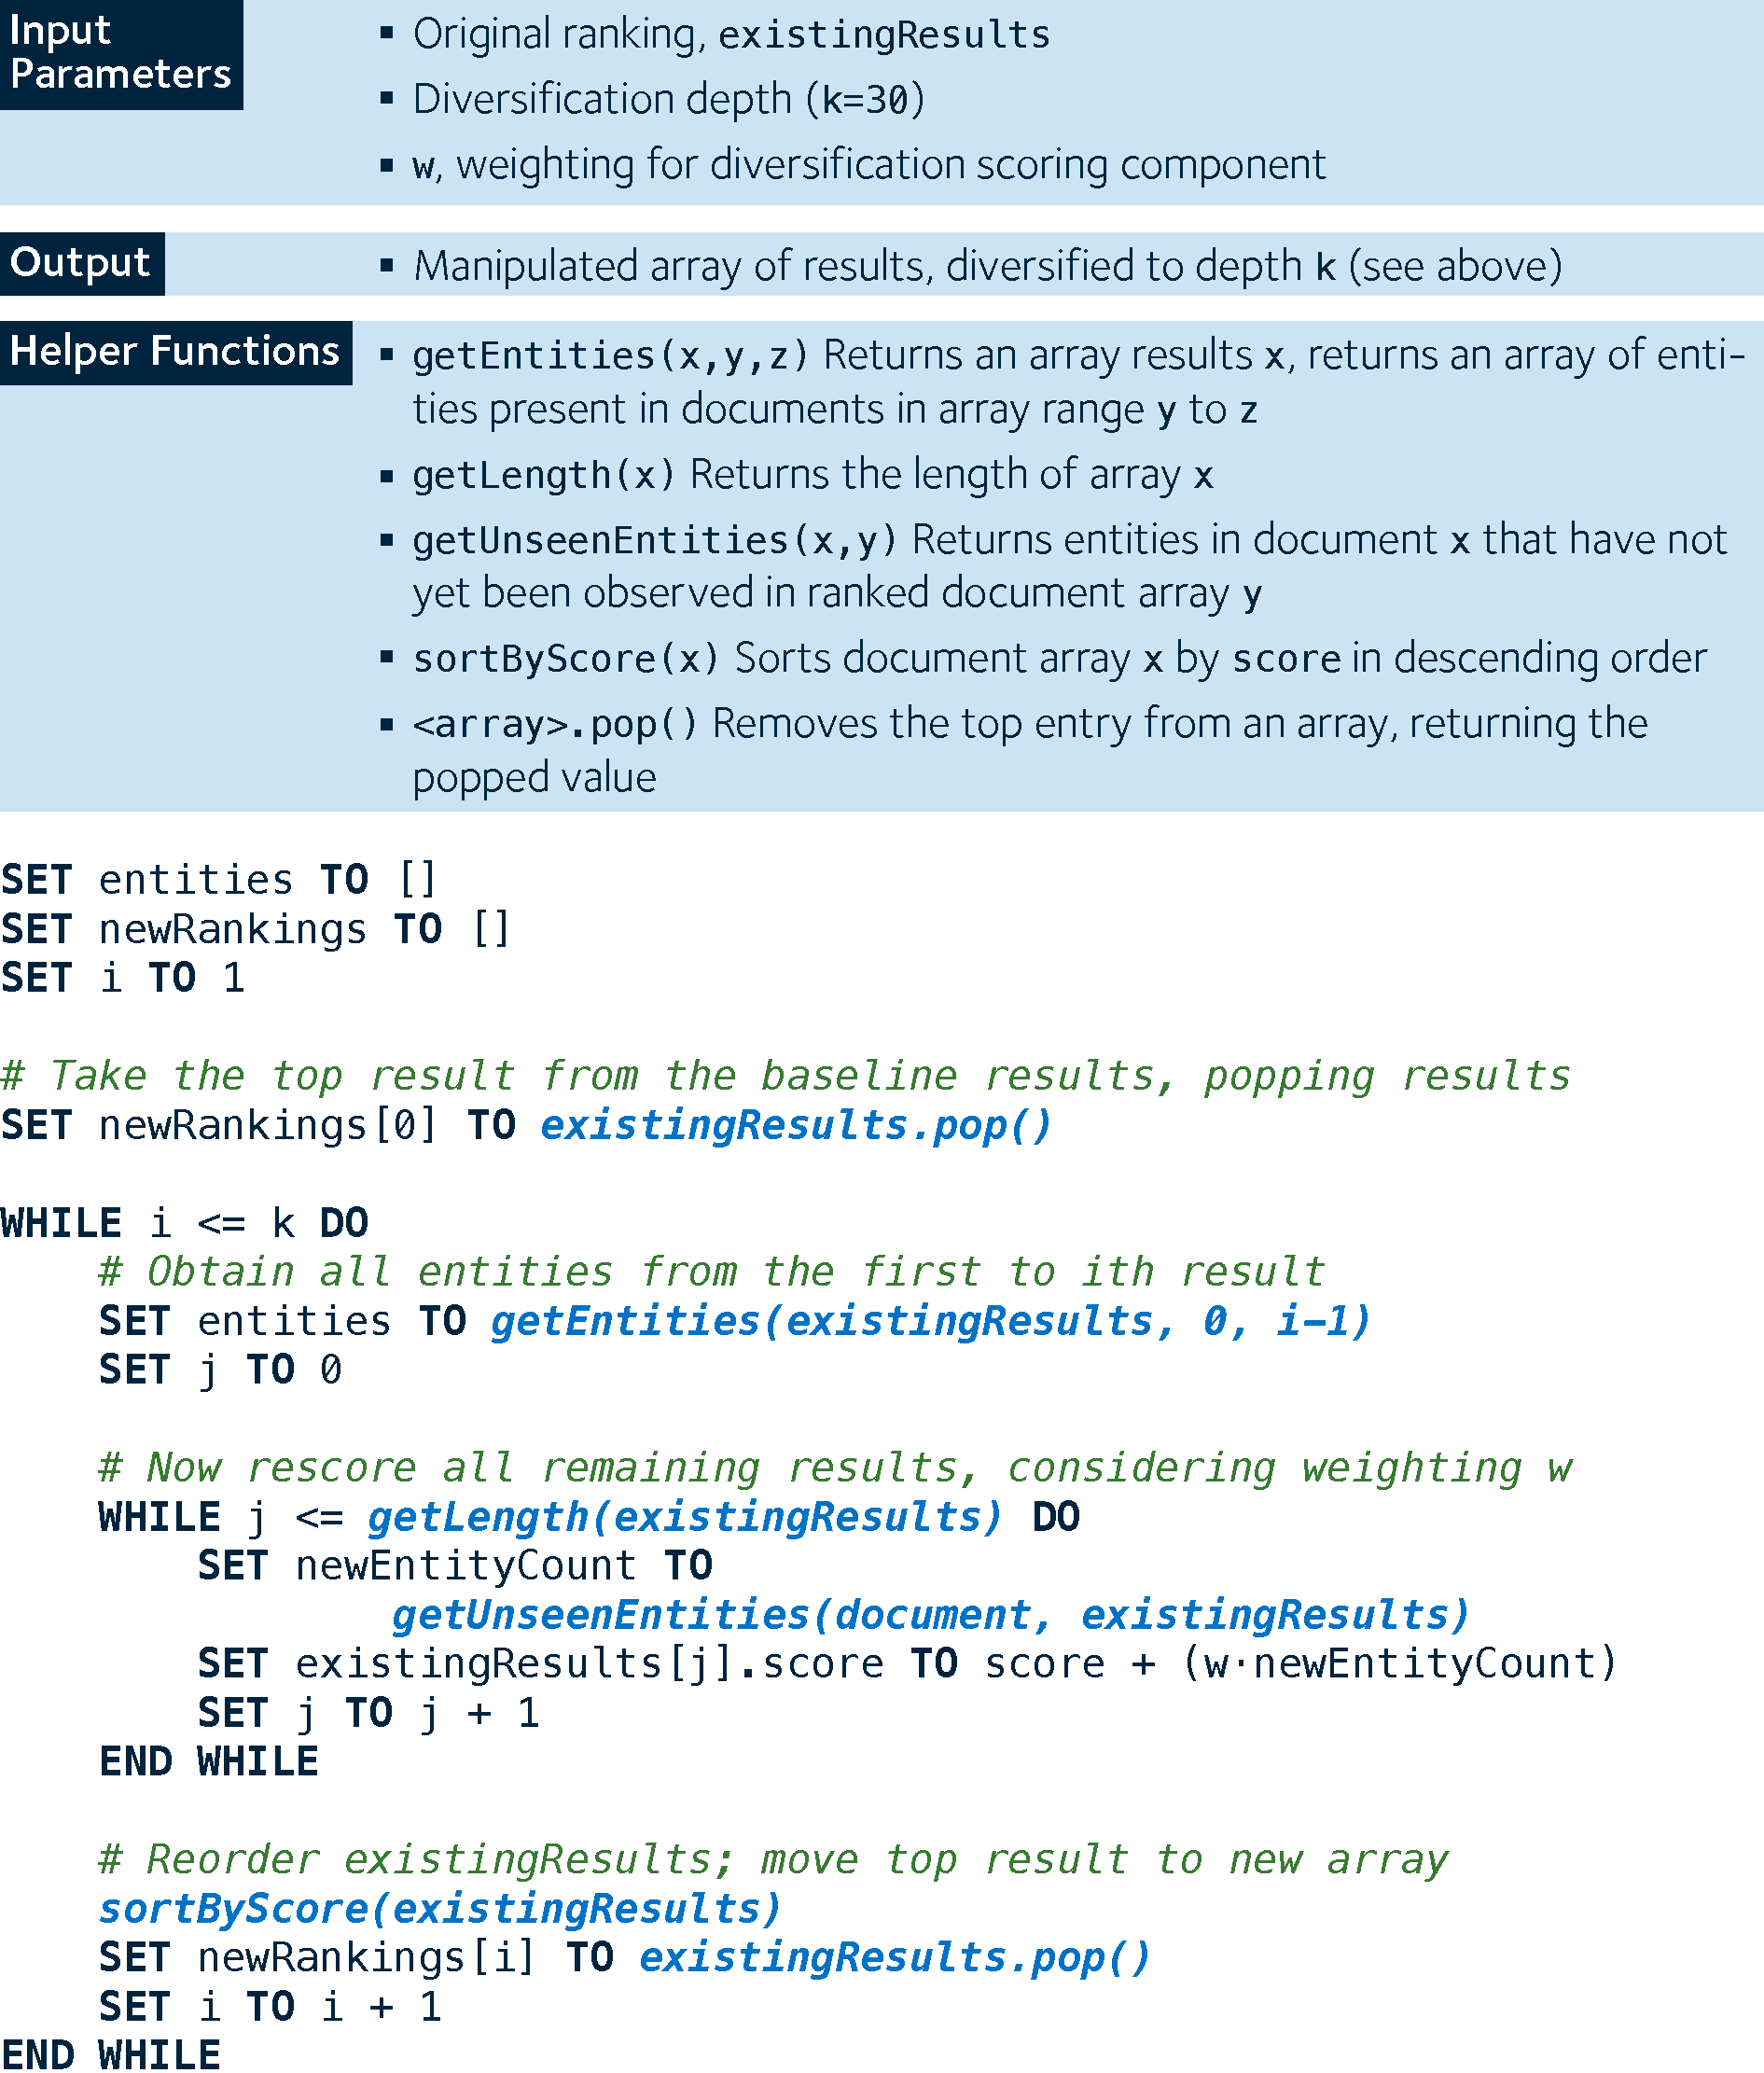
\includegraphics{figures/ch8-pseudocode.pdf}}
    \caption[Diversification algorithm pseudo-code]{Pseudo-code of the diversification algorithm used in this study, based upon the XQuAD framework by~\cite{santos2010query_reformulations_diversification}. As described in Section~\ref{sec:diversity:users:diversifying}, the algorithm guarantees that~\gls{acr:trec} relevant documents containing different aspects from each other will bubble up the baseline (BM25) rankings. Psuedo-code is provided in \emph{HAGGIS}~\citep{cutts2014haggis}.}
    \label{alg:diversifying}
\end{figure}
\renewcommand{\figurename}{Figure}

In order to select a reasonable approximation for the algorithm's $w$ weighting, we performed a pilot study, running the diversification algorithm over the set of $715$ queries that were issued by subjects of the user study reported in Chapter~\ref{chap:snippets}. Results of the pilot study are presented in Table~\ref{tbl:aspects_previous_queries}. As can be seen from the table, we explored a range of cutoff ($k$) and weighting ($w$) values, with $10-50$ trialled for $k$ and $0.1-1.0$ trialled for $w$. We selected $k=30, w=0.7$ as this combination provided the best results ($AR@10=6.61$, $\alpha DCG=0.075$, $P@10=0.36$) in terms of performance and efficiency. A higher $k$ for example only slightly increased performance, but took longer to compute. Indeed, $k=30$ was deemed to be a sensible choice as subjects from the prior user study didn't go lower than a depth of $24$ on average over interface \blueboxbold{T0}.

\begin{table}[t!]
    \caption[Aspectual recall pilot study results]{Table illustrating the effects of varying the diversification weighting parameter, \emph{w}, and diversification cutoff \emph{k} when using the diversification algorithm as discussed in Section~\ref{sec:diversity:users:diversifying}. Values in the table represent the aspectual recall in the top 10 documents \emph{(AR@10)} after re-ranking, on average, over the 715 queries issued by subjects of the user study reported in Chapter~\ref{chap:snippets}. At \emph{w=0.0}, diversification is not applied – this configuration therefore enjoys the same performance as our baseline, non-diversified system \blueboxbold{ND}, utilising BM25 \emph{(b=0.75).}\vspace*{-3mm}}
    \label{tbl:aspects_previous_queries}
    \renewcommand{\arraystretch}{1.8}
    \begin{center}
    \begin{tabulary}{\textwidth}{L{0.4cm}@{\CS}D{2cm}@{\CS}D{2.12cm}@{\CS}D{2.12cm}@{\CS}D{2.12cm}@{\CS}D{2.12cm}@{\CS}D{2.12cm}@{\CS}}
    
    & & \multicolumn{5}{c}{\hspace*{-5mm}\textbf{Cutoff Range (k)}}\\
    
    \RS & & \lbluecell\textbf{10} & \lbluecell\textbf{20} & \lbluecell\textbf{30} & \lbluecell\textbf{40} & \lbluecell\textbf{50}\\
    
    \RS \multirow{7}{*}{\rotatebox{90}{\hspace*{-10mm}\textbf{Weighting Parameter}}} & \lbluecell\textbf{0.0 (ND)} & \multicolumn{5}{@{\hskip 0pt}c@{\CS}}{\dbluecell 3.64} \\
    
    \RS & \lbluecell\textbf{0.1} & \cell 3.64 & \cell 4.94 & \cell 5.51 & \cell 5.95 & \cell 6.37 \\
    \RS & \lbluecell\textbf{0.3} & \cell 6.58 & \cell 6.58 & \cell 6.64 & \cell 6.59 & \cell 6.59 \\
    \RS & \lbluecell\textbf{0.5} & \cell 6.58 & \cell 6.58 & \cell 6.58 & \cell 5.58 & \cell 6.58 \\
    \RS & \lbluecell\textbf{0.7 (D)} & \cell 6.56 & \cell 6.56 & \dbluecell 6.61 & \cell 6.51 & \cell 6.60 \\
    \RS & \lbluecell\textbf{0.9} & \cell 6.52 & \cell 6.52 & \cell 6.61 & \cell 6.57 & \cell 6.63 \\
    \RS & \lbluecell\textbf{1.0} & \cell 6.63 & \cell 6.63 & \cell 6.59 & \cell 6.61 & \cell 6.56 \\
    
\end{tabulary}
\end{center}
\end{table}

For the diversity re-ranking to work in this scenario, the algorithm must be aware of the ground truths which were collated, as described in Section~\ref{sec:diversity:users:method:aspects} above. The reasons for following this approach were:

\begin{itemize}
    \item{us not having to invest a significant amount of effort tuning a different diversification algorithm to return acceptable results; and}
    \item{that it would guarantee that~\gls{acr:trec} relevant documents, containing different entities, would bubble up to the top of the rankings, increasing the effect (and hopefully subject observation) that the results were indeed ranked differently.}
\end{itemize}

Without such a ground truth based approach, ensuring that~\gls{acr:trec} relevant documents would bubble up would have been difficult to achieve. Given the effects of document pooling as part of how the~\gls{acr:trec} QRELs were created (refer to Section~\ref{sec:ir_background:paradigms:trec}), it is highly likely that many other documents exist within the corpus that could be considered to be useful to a given topic, but were not assessed.

As previously discussed, one major pitfall of this approach is that the diversification algorithm employed would have provided results that were \emph{too good,} thus not presenting much of a challenge to subjects. To mitigate this issue, we also included documents that were considered non-relevant by~\gls{acr:trec} assessors (i.e. a~\gls{acr:trec} assessment of $0$) when performing re-ranking. This led to including an additional $2,663$ documents that would be included within the diversity re-ranking, but were not relevant. For the five topics we considered, the number of non-relevant documents from the~\gls{acr:trec} QRELs over each topic were reported in Table~\ref{tbl:ch6_topic_rels} on page~\pageref{tbl:ch6_topic_rels}.

Rather than manually assess each non-relevant document, we took the list of entities that were discovered for~\gls{acr:trec} relevant documents, and performed an exact keyword search for each of the entities within each of the $2,663$ documents. Any matches would have the corresponding entity attached to the document.

% \blueboxheader{Avoiding Perfect Results}
% As previously discussed, one major pitfall of this approach is that the diversification algorithm would have become \emph{too perfect.} With access to the ground truths, it would subsequently proceed to assign a higher rank to documents that were~\gls{acr:trec} assessed, leading to every document in the top $k$ containing new entities. To make this more of a challenge for subjects, We also incorporated within our aspectual data for ranking documents that were considered to be non-relevant by~\gls{acr:trec} assessors (i.e. a~\gls{acr:trec} assessment of $0$). This led to including an additional $2,663$ document that would be included within the diversity re-ranking, but were not relevant. For each of the five topics we consider in this thesis, the number of non-relevant documents from the~\gls{acr:trec} QRELs over each topic were:
%
% \begin{itemize}
%     \item{\blueboxbold{Airport Security} with 580 non-relevant documents;}
%     \item{\blueboxbold{Wildlife Extinction} with 500 non-relevant documents;}
%     \item{\blueboxbold{Piracy} with 526 non-relevant documents;}
%     \item{\blueboxbold{Tropical Storms} with 502 non-relevant documents; and}
%     \item{\blueboxbold{Curbing Population Growth} with 555 non-relevant documents.}
% \end{itemize}
%
% Rather than manually assess each document, we took the list of entities that were discovered for~\gls{acr:trec} relevant documents, and performed an exact keyword search for each of the entities within each of the $2,663$ documents. Any matches would have the corresponding entity attached to the document.

\subsubsection{Post-Task Surveys}\label{sec:diversity:users:posttask}
With the pre-task survey the same as that outlined in the general methodology (refer to Section~\ref{sec:methodology:extracting:user}), surveys for this study differed post-task and post-experiment. Here, we discuss the questions posed in each of the four post-task surveys.

On the completion of each of the four search tasks, subjects were asked to answers questions that were split into two broad categories, examining:

\begin{itemize}
    \item{their perceived behaviours when interacting; and}
    \item{how they felt the retrieval system they used had performed.}
\end{itemize}

Answers were compulsory; we provided a seven-point Likert scale for responses, providing the ability to give a neutral response, as well as strong disagreement \emph{(1)} or agreement \emph{(7)} with the questions that were posed.

Considering the subject's behaviours, we asked their opinions on the following areas.

\begin{itemize}
    \item{\blueboxbold{Success} How successful they thought they were at completing the given search task.}
    \item{\blueboxbold{Subject Speed} How quickly subjects felt that they completed the search task.}
    \item{\blueboxbold{Queries} Whether the subjects issued different queries to explore the topic.}
    \item{\blueboxbold{Documents} If they only examined a small number of documents per query.}
    \item{\blueboxbold{Checks} Whether they checked each document carefully before saving.}
    \item{\blueboxbold{Enough} Whether the subjects saved more documents than was required (remembering that subjects were instructed to save a minimum of four per task).}
\end{itemize}

In addition to the behavioural component of the survey, the system-sided component of the survey asked an additional six questions, again using a seven-point Likert scale. The questions posed to the subjects are enumerated below.

\begin{itemize}
    \item{\blueboxbold{System Speed} How well subjects thought the system helped them complete the given search task quickly.}
    \item{\blueboxbold{Difficulty} Whether they felt the system made things difficult to find useful information.}
    \item{\blueboxbold{Ease} If the system made it easy for subjects to complete the given search task.}
    \item{\blueboxbold{Happiness} Whether the subjects were happy or not with how the system performed.}
    \item{\blueboxbold{Cumbersome} Whether they felt the system was cumbersome to use or not.}
    \item{\blueboxbold{Confidence} How confident the subjects were in the decisions that they had taken.}
\end{itemize}

\subsubsection{Post-Experiment Survey}\label{sec:diversity:users:postexp}
In addition to the post-task surveys, we also asked subjects to answer a post-experiment survey upon completion of all four search tasks. Here, we wanted to ascertain which of the two retrieval systems (\hula, representing the baseline, non-diversified system \blueboxbold{ND} or \yoyo~Search, representing the diversified system, \blueboxbold{D}) offered subjects a better experience, and which one of the two that they preferred overall.

Seven questions were posed, with answers again provided on a Likert scale. However, we this time provided six possible choices, from $1$ (definitely \hula) to $3$ (slightly \hula), from $4$ (slightly \yoyo) to $6$ (definitely \yoyo). We opted not to include a neutral option to force subjects into deciding between one of the two systems. We asked the subjects the following questions.

\begin{itemize}
    \item{\blueboxbold{Informative} Of the two retrieval systems, subjects were asked to pick which of the two returned the most informative results.}
    \item{\blueboxbold{Unhelpful} What one of the two retrieval systems was the most unhelpful?}
    \item{\blueboxbold{Easiest} Of the two retrieval systems, what one was the easiest to use?}
    \item{\blueboxbold{Least Useful} Which retrieval system was the least useful?}
\end{itemize}

The final three questions then led on to asking subjects about what one of the two systems they felt yielded the most relevant and diverse content.

\begin{itemize}
    \item{\blueboxbold{Most Relevant} Which of the two retrieval systems yielded the most relevant information?}
    \item{\blueboxbold{Most Diverse} Which of the two retrieval systems offered the more diverse set of results?}
    \item{\blueboxbold{Most Preferable} Which retrieval system did you prefer overall?}
\end{itemize}

While responses from subjects did definitely provide a preferred retrieval system, we nevertheless discuss the results from this survey in Section~\ref{sec:diversity:users:results:experience}.

\subsection{Results}
We now move onto an analysis of the user study results, addressing the overarching study research question and chapter hypotheses posed in Section~\ref{sec:diversity:background:tasks:hypotheses}. In this analysis, we examine both the behaviour and performance of each subject across the four different experimental conditions, \dualbluebox{D}{AS}, \dualbluebox{ND}{AS}, \dualbluebox{D}{AD} and \dualbluebox{ND}{AD}. Both task (considering \blueboxbold{AD} vs. \blueboxbold{AS}) and system (considering \blueboxbold{ND} and \blueboxbold{D}) effects were also examined. To evaluate these data, ANOVAs were conducted using the experimental conditions, tasks and systems each as factors; main effects were examined with $\alpha=0.05$. Bonferroni tests were then used for post-hoc analysis where required. To reiterate, as discussed in Section~\ref{sec:diversity:users:measures}, $\alpha DCG$ is computed at $\alpha=0.5$.

\begin{table}[t!]
    \caption[Query performance over retrieval systems \blueboxbold{ND} and \blueboxbold{D}]{Query statistics and performance measures across both of the experimental systems trialled, \blueboxbold{ND} (baseline, non-diversified) and \blueboxbold{D} (diversified). Note the significant differences between the diversity-centric measures, $\alpha$DCG (where $\alpha$=0.5) and aspectual recall (AR), highlighting that the diversification algorithm did indeed provide subjects with a more diverse set of results with which to examine.\vspace*{-3mm}}
    \label{tbl:aspects_system_comparison}
    \renewcommand{\arraystretch}{1.8}
    \begin{center}
    \begin{tabulary}{\textwidth}{L{0.4cm}@{\CS}L{5.3cm}@{\CS}D{4.5cm}@{\CS}D{4.5cm}@{\CS}}
    
    & & \lbluecell \textbf{ND} & \lbluecell \textbf{D} \\
    
    \RS & \lbluecell\textbf{Queries Issued} & \cell 718 & \cell 555 \\
    \RS & \lbluecell\textbf{Terms per Query} & \cell 3.59 & \cell 3.80 \\
    \RS & \lbluecell\textbf{Unique Terms} & \cell 345 & \cell 292 \\
    
    \RS\RS\RS \multirow{2}{*}{\rotatebox{90}{\hspace*{-3mm}\textbf{Precision}}} & \lbluecell\textbf{P@5} & \cell 0.25$\pm$0.01* & \cell 0.29$\pm$0.01* \\
    \RS & \lbluecell\textbf{P@10} & \cell 0.22$\pm$0.01 & \cell 0.24$\pm$0.01 \\
    
    \RS\RS\RS \multirow{2}{*}{\rotatebox{90}{\hspace*{-3mm}\textbf{$\alpha$DCG}}} & \lbluecell\textbf{$\alpha$DCG@5} & \cell 0.02$\pm$0.00* & \cell 0.04$\pm$0.00* \\
    \RS & \lbluecell\textbf{$\alpha$DCG@10} & \cell 0.03$\pm$0.00* & \cell 0.04$\pm$0.00* \\
    
    \RS\RS\RS \multirow{2}{*}{\rotatebox{90}{\hspace*{-2mm}\textbf{AR}}} & \lbluecell\textbf{AR@5} & \cell 1.40$\pm$0.11* & \cell 3.39$\pm$0.21* \\
    \RS & \lbluecell\textbf{AR@10} & \cell 2.11$\pm$0.14* & \cell 4.07$\pm$0.24* \\
    
\end{tabulary}
\end{center}
\end{table}

To begin our analysis, we first examined whether the performance experienced by subjects over the two retrieval systems was in fact different, as indicated it would be by our pilot study (refer to Section~\ref{sec:diversity:users:diversifying}). We took the queries subjects issued to each of the two systems, and measured the performance according to $\alpha DCG$, AR and precision. Results are presented in Table~\ref{tbl:aspects_system_comparison}. Statistical testing confirms that the two systems were significantly different in terms of diversity (i.e. $\alpha DCG@10$: $F(1, 1272=28.74, p<0.001)$ and $AR@10$: $F(1,1272 = 55.43, p<0.001)$. However, $P@10$ was not significantly different between the two retrieval systems. This suggests that the re-ranking promoted relevant and diverse documents, but only from the top ten results (on average).

Aside from showing query performance, Table~\ref{tbl:aspects_system_comparison} also reports the number of terms issued per query over retrieval systems \blueboxbold{ND} and \blueboxbold{D}. Of the $1273$ total queries issued, those issued to \blueboxbold{ND} were shorter on average, with $3.59$ terms compared to $3.80$ terms for system \blueboxbold{D}. However, the vocabulary used by subjects issuing queries to \blueboxbold{ND} was greater than \blueboxbold{D} -- queries issued to \blueboxbold{ND} contained a total of $345$ unique terms, compared to $292$. This provides our first finding of note from the data. When using retrieval system \blueboxbold{ND} that did not diversify search results, subjects issued a greater number of queries -- but were slightly shorter and more varied -- in order to accomplish their tasks.

\subsubsection{Interaction Measures}
Firstly, we examine the different interactions between searchers and the retrieval systems. Tables~\ref{tbl:aspectual_combo_beperftime} and~\ref{tbl:aspectual_system_tasks_beperftime} both present the mean (and standard deviations) of:

\begin{itemize}
    \item{the number of queries issued \emph{(Queries Issued);}}
    \item{the number of~\glsplural{acr:serp} that were examined by subjects per query \emph{(\#\glsplural{acr:serp}/Q);}}
    \item{the number of documents examined (clicked) per query \emph{(\#Docs/Q.);} and}
    \item{the click depth (or stopping depth) per query \emph{(Depth/Q.).}}
\end{itemize}

These are reported in the \genericblack{Interactions} category in both tables. Table~\ref{tbl:aspectual_combo_beperftime} reports over the four different system and task combinations trialled, while Table~\ref{tbl:aspectual_system_tasks_beperftime} reports over each individual system and task. Statistical tests reveal no effects across conditions, systems or tasks. However, there are several trends that are worth discussing. Firstly, we notice that when subjects used the diversified system \blueboxbold{D} to complete the aspectual retrieval task, they examined fewer documents per query than when completing the same task on the non-diversified system \blueboxbold{ND} ($12.85$ vs. $15.73$) -- which is in line with \darkblueboxbold{H1}. We also observed that subjects issued slightly more queries on \blueboxbold{D} compared to \blueboxbold{ND} under the aspectual retrieval task ($5.92$ vs. $5.25$). This is in line with \darkblueboxbold{H2a} -- these results however were not statistically significant.

Now we turn our attention to the ad-hoc retrieval tasks. Our hypotheses suggested that there would be no differences in terms of the number of documents examined \darkblueboxbold{H3}, or in the number of queries issued \darkblueboxbold{H4} -- which was the case. However, we note that subjects using \blueboxbold{D} inspected more results than when using \blueboxbold{ND} ($16.19$ vs. $13.94$), and they issued slightly fewer queries ($4.96$ vs. $5.20$). We can see the trade-offs between queries and the number of results inspected per query, where more queries tends to lead to fewer results being examined, and vice versa. This trend suggests that subjects, when searching using diversified system \blueboxbold{D}, under an ad-hoc task, may have had to dig deeper to find more relevant material, due to the system's performance. Alternatively, this trend could be explained by suggesting that the system encouraged subjects to go deeper, something that we intuitively expected when subjects were searching for aspectual, diversified information. Either way, no conclusive evidence to support our hypotheses exists -- merely trends.

\begin{table}[t!]
    \caption[Behaviour and performance over experimental conditions]{Behavioural (including interaction and time-based) and performance measures, across each of the experimental conditions \dualbluebox{D}{AS}, \dualbluebox{ND}{AS}, \dualbluebox{D}{AD} and \dualbluebox{ND}{AD}.}
    \label{tbl:aspectual_combo_beperftime}
    \renewcommand{\arraystretch}{1.8}
    \begin{center}
    \begin{tabulary}{\textwidth}{L{0.4cm}@{\CS}L{3.2cm}@{\CS}D{2.5cm}@{\CS}D{2.5cm}@{\CS}D{2.5cm}@{\CS}D{2.5cm}@{\CS}}

        & & \lbluecell \textbf{D-AS} & \lbluecell \textbf{ND-AS} & \lbluecell \textbf{D-AD} & \lbluecell \textbf{ND-AD} \\

        \RS \multirow{4}{*}{\rotatebox{90}{\hspace*{-5mm}\textbf{Interactions}}} & \lbluecell\textbf{\#Queries} & \cell \small{5.92$\pm$0.88} & \cell \small{5.25$\pm$0.80} & \cell \small{4.96$\pm$0.74} & \cell \small{5.20$\pm$0.69}\\
        \RS & \lbluecell\textbf{\#\glsplural{acr:serp}/Query} & \cell \small{1.78$\pm$0.14} & \cell \small{2.42$\pm$0.24} & \cell \small{2.28$\pm$0.31} & \cell \small{2.28$\pm$0.20}\\
        \RS & \lbluecell\textbf{\#Docs./Query} & \cell \small{3.02$\pm$0.39} & \cell \small{3.65$\pm$0.46} & \cell \small{3.48$\pm$0.51} & \cell \small{3.23$\pm$0.37}\\
        \RS & \lbluecell\textbf{Depth/Query} & \cell \small{12.85$\pm$1.49} & \cell \small{15.73$\pm$1.45} & \cell \small{16.19$\pm$2.14} & \cell \small{13.94$\pm$1.93}\\
        
        \RS\RS\RS \multirow{5}{*}{\rotatebox{90}{\hspace*{-6mm}\textbf{Performance}}} & \lbluecell\textbf{\#Saved} & \cell \small{5.80$\pm$0.26} & \cell \small{5.96$\pm$0.25} & \cell \small{5.92$\pm$0.25} & \cell \small{5.78$\pm$0.20}\\
        \RS & \lbluecell\textbf{\#\gls{acr:trec} Saved} & \cell \small{2.63$\pm$0.22} & \cell \small{2.18$\pm$0.23} & \cell \small{2.51$\pm$0.23} & \cell \small{2.22$\pm$0.22}\\
        \RS & \lbluecell\textbf{\#\gls{acr:trec} Non.} & \cell \small{1.75$\pm$0.22} & \cell \small{1.96$\pm$0.23} & \cell \small{1.37$\pm$0.22} & \cell \small{1.82$\pm$0.23 }\\
        \RS & \lbluecell\textbf{\#Ent. Found} & \cell \small{7.22$\pm$0.94*} & \cell \small{4.31$\pm$0.60*} & \cell \small{5.82$\pm$0.77} & \cell \small{4.37$\pm$0.59*}\\
        \RS & \lbluecell\textbf{\#Docs. New Ent.} & \cell \small{3.20$\pm$0.21*} & \cell \small{2.35$\pm$0.20*} & \cell \small{2.63$\pm$0.23} & \cell \small{2.02$\pm$0.18*}\\
        
        \RS\RS\RS \multirow{5}{*}{\rotatebox{90}{\hspace*{3mm}\textbf{Times}}} & \lbluecell\textbf{Total Session} & \cell \small{443.65$\pm$45.05} & \cell \small{430.50$\pm$38.39} & \cell \small{432.18$\pm$49.87} & \cell \small{447.55$\pm$47.82}\\
        \RS & \lbluecell\textbf{Per Query} & \cell \small{8.80$\pm$0.89} & \cell \small{9.99$\pm$1.21} & \cell \small{9.69$\pm$0.79} & \cell \small{8.69$\pm$0.57}\\
        \RS & \lbluecell\textbf{Per Document} & \cell \small{15.97$\pm$1.96} & \cell \small{13.03$\pm$1.01} & \cell \small{13.66$\pm$1.02} & \cell \small{15.09$\pm$2.20}\\
        \RS & \lbluecell\textbf{Per Summary} & \cell \small{1.59$\pm$0.09} & \cell \small{1.75$\pm$0.15} & \cell \small{1.71$\pm$0.11} & \cell \small{1.71$\pm$0.13}\\
        
    \end{tabulary}
    \end{center}
\end{table}

\begin{table}[t!]
    \caption[Behaviour and performance over systems and tasks]{Behavioural (including interaction and time-based) and performance measures, across the two experimental systems \blueboxbold{ND} and \blueboxbold{D}, as well as the two tasks, \blueboxbold{AD} and \blueboxbold{AS}.}
    \label{tbl:aspectual_system_tasks_beperftime}
    \renewcommand{\arraystretch}{1.8}
    \begin{center}
    \begin{tabulary}{\textwidth}{L{0.4cm}@{\CS}L{3.2cm}@{\CS}D{2.5cm}@{\CS}D{2.5cm}@{\CS}D{2.5cm}@{\CS}D{2.5cm}@{\CS}}

        & & \lbluecell \textbf{ND} & \lbluecell \textbf{D} & \lbluecell \textbf{AD} & \lbluecell \textbf{AS} \\

        \RS \multirow{4}{*}{\rotatebox{90}{\hspace*{-5mm}\textbf{Interactions}}} & \lbluecell\textbf{\#Queries} & \cell \small{5.23$\pm$0.53} & \cell \small{5.44$\pm$0.58} & \cell \small{5.08$\pm$0.51} & \cell \small{5.59$\pm$0.59}\\
        \RS & \lbluecell\textbf{\#\glsplural{acr:serp}/Query} & \cell \small{2.35$\pm$0.16} & \cell \small{2.03$\pm$0.17} & \cell \small{2.28$\pm$0.18} & \cell \small{2.10$\pm$0.14}\\
        \RS & \lbluecell\textbf{\#Docs/Query} & \cell \small{3.44$\pm$0.29} & \cell \small{3.25$\pm$0.32} & \cell \small{3.36$\pm$0.31} & \cell \small{3.34$\pm$0.30}\\
        \RS & \lbluecell\textbf{Depth/Query} & \cell \small{14.84$\pm$1.58} & \cell \small{14.52$\pm$1.31} & \cell \small{15.07$\pm$1.44} & \cell \small{14.29$\pm$1.47}\\
        
        \RS\RS\RS \multirow{5}{*}{\rotatebox{90}{\hspace*{-6mm}\textbf{Performance}}} & \lbluecell\textbf{\#Saved} & \cell \small{5.87$\pm$0.16} & \cell \small{5.86$\pm$0.18} & \cell \small{5.85$\pm$0.16} & \cell \small{5.88$\pm$0.18}\\
        \RS & \lbluecell\textbf{\#\gls{acr:trec} Saved} & \cell \small{2.20$\pm$0.16} & \cell \small{2.57$\pm$0.16} & \cell \small{2.36$\pm$0.16} & \cell \small{2.40$\pm$0.16}\\
        \RS & \lbluecell\textbf{\#\gls{acr:trec} Non.} & \cell \small{1.89$\pm$0.16} & \cell \small{1.56$\pm$0.16} & \cell \small{1.60$\pm$0.16} & \cell \small{1.85$\pm$0.16}\\
        \RS & \lbluecell\textbf{\#Ent. Found} & \cell \small{4.34$\pm$0.42*} & \cell \small{6.52$\pm$0.61*} & \cell \small{5.10$\pm$0.49} & \cell \small{5.76$\pm$0.57}\\
        \RS & \lbluecell\textbf{\#Docs. New Ent.} & \cell \small{2.19$\pm$0.13*} & \cell \small{2.91$\pm$0.16*} & \cell \small{2.32$\pm$0.15*} & \cell \small{2.77$\pm$0.15*}\\
        
        \RS\RS\RS \multirow{5}{*}{\rotatebox{90}{\hspace*{3mm}\textbf{Times}}} & \lbluecell\textbf{Total Session} & \cell \small{439.02$\pm$30.52} & \cell \small{437.91$\pm$33.44} & \cell \small{439.86$\pm$34.38} & \cell \small{437.08$\pm$29.45}\\
        \RS & \lbluecell\textbf{Per Query} & \cell \small{9.34$\pm$0.67} & \cell \small{9.25$\pm$0.59} & \cell \small{9.19$\pm$0.49} & \cell \small{9.39$\pm$0.75}\\
        \RS & \lbluecell\textbf{Per Document} & \cell \small{14.06$\pm$1.21} & \cell \small{14.81$\pm$1.10} & \cell \small{14.37$\pm$1.21} & \cell \small{14.50$\pm$1.11}\\
        \RS & \lbluecell\textbf{Per Summary} & \cell \small{1.73$\pm$0.10} & \cell \small{1.65$\pm$0.07} & \cell \small{1.71$\pm$0.08} & \cell \small{1.67$\pm$0.09}\\
        
    \end{tabulary}
    \end{center}
\end{table}

\subsubsection{Performance Measures}
Tables~\ref{tbl:aspectual_combo_beperftime} and~\ref{tbl:aspectual_system_tasks_beperftime} also report a number of different performance measures, reported within the \genericblack{Performance} grouping. Included in these tables are:

\vspace*{-5mm}
\begin{itemize}
    \item{the number of saved documents \emph{(\#Saved);} also broken down into:}
    
    \begin{itemize}
        \item{the number that were~\gls{acr:trec} relevant \emph{(\#\gls{acr:trec} Saved);} and}
        \item{the number that were~\gls{acr:trec} non-relevant \emph{(\#\gls{acr:trec} Non);}}
    \end{itemize}
    
    \item{the number of new entities that were found (within saved documents, with new entities being in the context of a search session) \emph{(\#Ent. Found);} and}
    \item{the number of documents containing at least one new entity \emph{(\#Docs. New Ent.).}}
\end{itemize}

In terms of the number of documents saved, there were no significant differences between conditions, systems or tasks. On average, subjects saved around six documents on average, with was two more than the minimum goal of four. This suggests that subjects wanted to make sure that they found a few extra, potentially useful documents, just in case some of their other selections turned out to be not useful.

\begin{table}[t!]
    \caption[Interaction probabilities]{Interaction probabilities, as observed over the four experimental conditions. Refer to Section~\ref{sec:method:simulation:grounding:judgements} on page~\pageref{sec:method:simulation:grounding:judgements} for  an explanation of the different probabilities listed here.}
    \label{tbl:diversity_probabilities}
    \renewcommand{\arraystretch}{1.8}
    \begin{center}
    \begin{tabulary}{\textwidth}{L{0.4cm}@{\CS}L{3.2cm}@{\CS}D{2.5cm}@{\CS}D{2.5cm}@{\CS}D{2.5cm}@{\CS}D{2.5cm}@{\CS}}

        & & \lbluecell \textbf{D-AS} & \lbluecell \textbf{ND-AS} & \lbluecell \textbf{D-AD} & \lbluecell \textbf{ND-AD} \\

        \RS \multirow{3}{*}{\rotatebox{90}{\hspace*{-5mm}\textbf{Click}}} & \lbluecell\textbf{P(C)} & \cell \small{0.16$\pm$0.01*} & \cell \small{0.21$\pm$0.02*} & \cell \small{0.16$\pm$0.01*} & \cell \small{0.20$\pm$0.01*}\\
        \RS & \lbluecell\textbf{P(C|R)} & \cell \small{0.27$\pm$0.03} & \cell \small{0.30$\pm$0.04} & \cell \small{0.25$\pm$0.03} & \cell \small{0.31$\pm$0.04}\\
        \RS & \lbluecell\textbf{P(C|N)} & \cell \small{0.13$\pm$0.02*} & \cell \small{0.18$\pm$0.02*} & \cell \small{0.13$\pm$0.01*} & \cell \small{0.17$\pm$0.02*}\\
        
        \RS\RS\RS \multirow{3}{*}{\rotatebox{90}{\hspace*{-5mm}\textbf{Save}}} & \lbluecell\textbf{P(S)} & \cell \small{0.67$\pm$0.03} & \cell \small{0.66$\pm$0.03} & \cell \small{0.70$\pm$0.03} & \cell \small{0.71$\pm$0.04}\\
        \RS & \lbluecell\textbf{P(S|R)} & \cell \small{0.78$\pm$0.04} & \cell \small{0.63$\pm$0.05} & \cell \small{0.74$\pm$0.04} & \cell \small{0.67$\pm$0.05}\\
        \RS & \lbluecell\textbf{P(S|N)} & \cell \small{0.59$\pm$0.04} & \cell \small{0.61$\pm$0.04} & \cell \small{0.65$\pm$0.04} & \cell \small{0.65$\pm$0.04}\\
        
    \end{tabulary}
    \end{center}
\end{table}

When we turn our attention to the entity-related measures, we note that subjects found more documents that contained new entities, and found more new entities overall, when using the diversity system \blueboxbold{D}. This was statistically significant ($6.52\pm0.61$ compared to $4.34\pm0.42$ for systems \blueboxbold{D} and \blueboxbold{ND} respectively, where $F(1,203 = 8.70, p<0.05)$). When examining each condition, the Bonferroni follow-up test showed significant differences between conditions \dualbluebox{D}{AS} and conditions \dualbluebox{D}{AD} and \dualbluebox{ND}{AD}, where $F(3,203 = 3.49, p < 0.05)$. We also noticed that subjects found more documents with new entities, and thus more entities generally, for task \dualbluebox{D}{AD} than when using \blueboxbold{ND} (documents with new entities: $2.63$ vs. $2.02$, new entities: $5.82$ vs. $4.37$). Though this was not significantly different, it does suggest that when subjects used system \blueboxbold{D}, they did learn more about the different aspects of the given topic (or at least encountered more aspects) than when using system \blueboxbold{ND} that did not diversify results.

Table~\ref{tbl:diversity_probabilities} reports interaction probabilities associated with searcher interactions, the details of which are discussed in Section~\ref{sec:method:simulation:grounding:judgements} on page~\pageref{sec:method:simulation:grounding:judgements}. From the table, we can see that there was a significant difference between conditions for the probability of clicking on a result summary link, and the probability of clicking on~\gls{acr:trec} non-relevant items. Comparing systems indicated that subjects clicked more when using the non-diversified system, and clicked on more non-relevant documents. However, we did not observe any task effects, and thus do not report these measures here. This suggests that the non-diversified system \blueboxbold{ND} led to subjects examining more documents, but often more non-relevant documents. This is reflected by the fact that across all the performance measures, subjects, when using system \blueboxbold{ND}, performed worse.

\subsubsection{Time-Based Measures}
Tables~\ref{tbl:aspectual_combo_beperftime} and~\ref{tbl:aspectual_system_tasks_beperftime} also report a third grouping of results, showing a series of times recorded for various interactions. These are all reported in the \genericblack{Times} grouping. Across both tables (conditions, systems and tasks), we report:

\begin{itemize}
    \item{the mean total session time (denoted as from the first query focus to ending the task, \emph{Total Session);}}
    \item{the mean time spent entering queries \emph{(Per Query);}}
    \item{the mean per document examination time \emph{(Per Document);} and}
    \item{the mean time spent examining an individual result summary \emph{(Per Summary).}}
\end{itemize}

All values in the two tables for time-based measures are reported in seconds. Surprisingly, no significant differences were found between any of the comparisons over the total session times, the per query times, the per document times, and the individual result summary examination times. Results however do show a relatively constant mean session time over each of the four experimental conditions, as shown in Table~\ref{tbl:aspectual_combo_beperftime}. At $\approx 438.5$ seconds, this is around seven minutes on average -- in line with the time taken to find four documents in the previous user study reported in Chapter~\ref{chap:snippets}.

Considering \darkblueboxbold{H2b}, no evidence was found to support that task completion times were lower under the diversifying retrieval system with an aspectual retrieval task \dualbluebox{D}{AS}. From Table~\ref{tbl:aspectual_system_tasks_beperftime}, we can see that subjects in actuality spent slightly longer on the task, with $443$ seconds reported for \blueboxbold{D} vs. $430$ seconds for \blueboxbold{ND} -- essentially, the difference of examining approximately one document on average.

\subsubsection{User Experience Measures}\label{sec:diversity:users:results:experience}
There were no notable significant differences between conditions, tasks, or systems for any of the post-task surveys. For the post-experiment survey, subjects were roughly evenly split between their preference for system \blueboxbold{D} or \blueboxbold{ND} -- again with no significant differences. This finding suggests that despite the substantial (and significant) difference in aspectual recall and other system performance measures, between the systems, subjects seemed largely ambivalent to the different system's influences. Of course, however, their observed behaviours do suggest that the system (and task) did affect their performance.

\begin{table}[t!]
    \caption[Post-task survey results]{Results from the post-task surveys, consisting of both the behavioural- and system-based questions. Results shown are averages recorded for each of the four experimental conditions when considering the seven-point Likert scale. }
    \label{tbl:aspects_post_behavioural}
    \renewcommand{\arraystretch}{1.8}
    \begin{center}
    \begin{tabulary}{\textwidth}{L{0.4cm}@{\CS}L{3.2cm}@{\CS}D{2.5cm}@{\CS}D{2.5cm}@{\CS}D{2.5cm}@{\CS}D{2.5cm}@{\CS}}

        & & \lbluecell \textbf{D-AS} & \lbluecell \textbf{ND-AS} & \lbluecell \textbf{D-AD} & \lbluecell \textbf{ND-AD} \\

        \RS \multirow{6}{*}{\rotatebox{90}{\hspace*{-8mm}\textbf{Behavioural}}} & \lbluecell\textbf{Success} & \cell \small{5.90} & \cell \small{5.53} & \cell \small{5.98} & \cell \small{5.98}\\
        \RS & \lbluecell\textbf{Subject Speed} & \cell \small{4.24} & \cell \small{4.33} & \cell \small{4.61} & \cell \small{4.45}\\
        \RS & \lbluecell\textbf{Queries} & \cell \small{5.75} & \cell \small{5.35} & \cell \small{5.24} & \cell \small{5.47}\\
        \RS & \lbluecell\textbf{Documents} & \cell \small{2.78} & \cell \small{3.00} & \cell \small{2.67} & \cell \small{2.69}\\
        \RS & \lbluecell\textbf{Checks} & \cell \small{6.08} & \cell \small{6.10} & \cell \small{6.14} & \cell \small{6.02}\\
        \RS & \lbluecell\textbf{Enough} & \cell \small{5.00} & \cell \small{5.06} & \cell \small{4.84} & \cell \small{5.43}\\
        
        \RS\RS\RS \multirow{6}{*}{\rotatebox{90}{\hspace*{-8mm}\textbf{System}}} & \lbluecell\textbf{System Speed} & \cell \small{4.55} & \cell \small{4.16} & \cell \small{4.84} & \cell \small{4.42}\\
        \RS & \lbluecell\textbf{Difficulty} & \cell \small{3.78} & \cell \small{4.20} & \cell \small{3.31} & \cell \small{3.38}\\
        \RS & \lbluecell\textbf{Ease} & \cell \small{4.53} & \cell \small{4.00} & \cell \small{4.47} & \cell \small{4.32}\\
        \RS & \lbluecell\textbf{Happiness} & \cell \small{4.45} & \cell \small{4.18} & \cell \small{4.73} & \cell \small{4.46}\\
        \RS & \lbluecell\textbf{Cumbersome} & \cell \small{3.31} & \cell \small{3.50} & \cell \small{3.18} & \cell \small{3.00}\\
        \RS & \lbluecell\textbf{Confidence} & \cell \small{5.25} & \cell \small{5.04} & \cell \small{5.63} & \cell \small{5.36}\\
        
    \end{tabulary}
    \end{center}
\end{table}

\begin{table}[t!]
    \caption[Post-experiment survey results]{Raw results of the post-experiment survey, with values denoting the total number of subjects who selected a given point on the scale (columns) for each of the questions posed (rows). As a reminder, \yoyo~denotes system \blueboxbold{D}; \hula~denotes system \blueboxbold{ND}. The lower the value, the stronger the preference to \yoyo; the higher the value, the stronger the preference to \hula.}
    \label{tbl:aspects_post_experiment}
    \renewcommand{\arraystretch}{1.8}
    \begin{center}
    \begin{tabulary}{\textwidth}{L{3.2cm}@{\CS}D{1.635cm}@{\CS}D{1.635cm}@{\CS}D{1.635cm}@{\CS}D{1.635cm}@{\CS}D{1.635cm}@{\CS}D{1.635cm}@{\CS}}
        
        & \multicolumn{3}{@{\hskip 0pt}c@{\CS}}{\yoyocell \textbf{Definitely YoYo Search}} & \multicolumn{3}{@{\hskip 0pt}c@{\CS}}{\hulacell \textbf{Definitely Hula Search}} \\
        
        \RS & \yoyocellone\textbf{1} & \yoyocelltwo\textbf{2} & \yoyocellthree\textbf{3} & \hulacellthree\textbf{4} & \hulacelltwo\textbf{5} & \hulacellone\textbf{6} \\
        
        \RS \lbluecell\textbf{Most Informative} & \cell 5 & \cell 0 & \cell 20 & \cell 20 & \cell 0 & \cell 6 \\
        \RS \lbluecell\textbf{Most Unhelpful} & \cell 7 & \cell 0 & \cell 21 & \cell 17 & \cell 0 & \cell 6 \\
        \RS \lbluecell\textbf{Easiest} & \cell 7 & \cell 0 & \cell 18 & \cell 20 & \cell 0 & \cell 6 \\
        \RS \lbluecell\textbf{Least Useful} & \cell 6 & \cell 0 & \cell 20 & \cell 18 & \cell 0 & \cell 7 \\
        \RS \lbluecell\textbf{Most Relevant} & \cell 10 & \cell 0 & \cell 16 & \cell 18 & \cell 0 & \cell 7 \\
        \RS \lbluecell\textbf{Most Diverse} & \cell 8 & \cell 0 & \cell 18 & \cell 19 & \cell 0 & \cell 6 \\
        \RS \lbluecell\textbf{Most Preferable} & \cell 9 & \cell 0 & \cell 16 & \cell 18 & \cell 0 & \cell 8 \\
    \end{tabulary}
    \end{center}
    \vspace*{-3mm}
\end{table}

\blueboxheader{Post-Task Surveys} Table~\ref{tbl:aspects_post_behavioural} provide the results of the post-task surveys, split between behavioural and system-sided questions. Questions were outlined previously in Section~\ref{sec:diversity:users:posttask}. To recap, a seven-point Likert scale was used for all responses, ranging from $1$ (strongly disagree) to $7$ (strongly agree). Turning our attention first to the behavioural survey results, we observed no significant differences across conditions, systems or tasks. However, across all conditions, systems and tasks, subjects broadly agreed with the statements that they were presented with, suggesting that they felt successful in completing the search tasks, and were able to complete them quickly. All were in agreement that they carefully checked their documents for usefulness (i.e. relevance and/or new entities, depending upon the task) before saving, but were in broad disagreement that they had examined a \emph{few} documents per query, indicating that across all conditions, subjects felt as though they had examined more than they felt they needed to.

Regarding the system-sided survey questions presented in Table~\ref{tbl:aspects_post_behavioural}, subjects considered that both systems offered a reasonably quick and straightforward approach to finding results, with a generally positive outcome, too. The systems generally did not appear to be considered cumbersome to use, and subjects did not find the system made it overly difficult to complete the tasks -- a significant difference existed between the two tasks for this question, where $F(1, 201=5.51, p<0.05)$. Overall, subjects felt happy with how the system performed, and thus appeared to show some confidence in their decisions.

\blueboxheader{Post-Experiment Survey}
Upon finishing the experiment, subjects completed the post-experiment survey as detailed in Section~\ref{sec:diversity:users:postexp}. Here, we asked subjects what one of the two systems they preferred (from either the non-diversified or diversified systems) over a number of different questions. Results from the survey, as shown in Table~\ref{tbl:aspects_post_experiment}, provide a mixed picture -- no one system stood out as being more favourable to subjects, with all questions recording a near 50-50 split between the two. This is an interesting finding, as results -- especially from Table~\ref{tbl:aspects_system_comparison} on page~\pageref{tbl:aspects_system_comparison} -- showed that there was a significant difference between the two systems. Subjects simply had a difficult time attempting to determine what system appeared to be more favourable to them.

\subsubsection{Gain over Time}\label{sec:diversity:users:results:ift}
Back in Section~\ref{sec:diversity:background:tasks}, we motivated this study -- and indeed the wider work reported in this chapter -- using~\gls{acr:ift}, where we constructed a number of gain curves reflecting our beliefs about how the search performance experienced by subjects would look on each of the four combinations of system and task. This was done in order to generate our hypotheses outlined in Section~\ref{sec:diversity:background:tasks:hypotheses}. In this final section of the user study results, we examined how subjects performed over time for each of the experimental conditions trialled, allowing us to infer the gain curves. We then compare each of the curves generated with our initial expectations, shown in Figure~\ref{fig:ift_theory} on page~\pageref{fig:ift_theory}.

To create empirical gain curves, we plotted~\glsfirst{acr:cg} against time, where gain was defined to be either:

\begin{itemize}
    \item{the number of \blueboxbold{saved relevant documents} when considering \blueboxbold{ad-hoc retrieval} tasks; and}
    \item{the number of \blueboxbold{saved, relevant and different} documents for \blueboxbold{aspectual retrieval} tasks.}
\end{itemize}

These definitions are what constituted as a useful document for both of the tasks, defined previously in Section~\ref{sec:diversity:users:method:tasks}. As both of these definitions can be expressed in the same units, they can therefore be also plotted on the same axes.

Just like the expectation plots shown in Figure~\ref{fig:ift_theory} on page~\pageref{fig:ift_theory}, Figure~\ref{fig:ift_empirical} plots the corresponding \emph{empirical gain curves} for:

\begin{itemize}
    \item[\emph{(a)}]{the non-diversified system, \blueboxbold{ND}, over both search tasks;}
    \item[\emph{(b)}]{the diversified system, \blueboxbold{D}, over both search tasks;}
    \item[\emph{(c)}]{the aspectual search task for both retrieval systems; and}
    \item[\emph{(d)}]{the ad-hoc task for both retrieval systems.}
\end{itemize}

Compared to out expectations in Figure~\ref{fig:ift_theory} on page~\pageref{fig:ift_theory}, on visual inspection, we see that our predictions were roughly in line with the levels of~\gls{acr:cg} experienced by the subjects (on average). With Figure~\ref{fig:ift_empirical} \emph{(a)} for example, we hypothesised that on retrieval system \blueboxbold{ND}, subjects would have experienced greater levels of gain. The empirical gain curves demonstrate that this actually occurred. A critical difference however though is for plot \emph{(b)}. Here, it is clear that subjects went through a very different experience when searching, motivating a revision of our expectations.

\begin{figure}[t!]
    \centering
    \resizebox{1\hsize}{!}{
    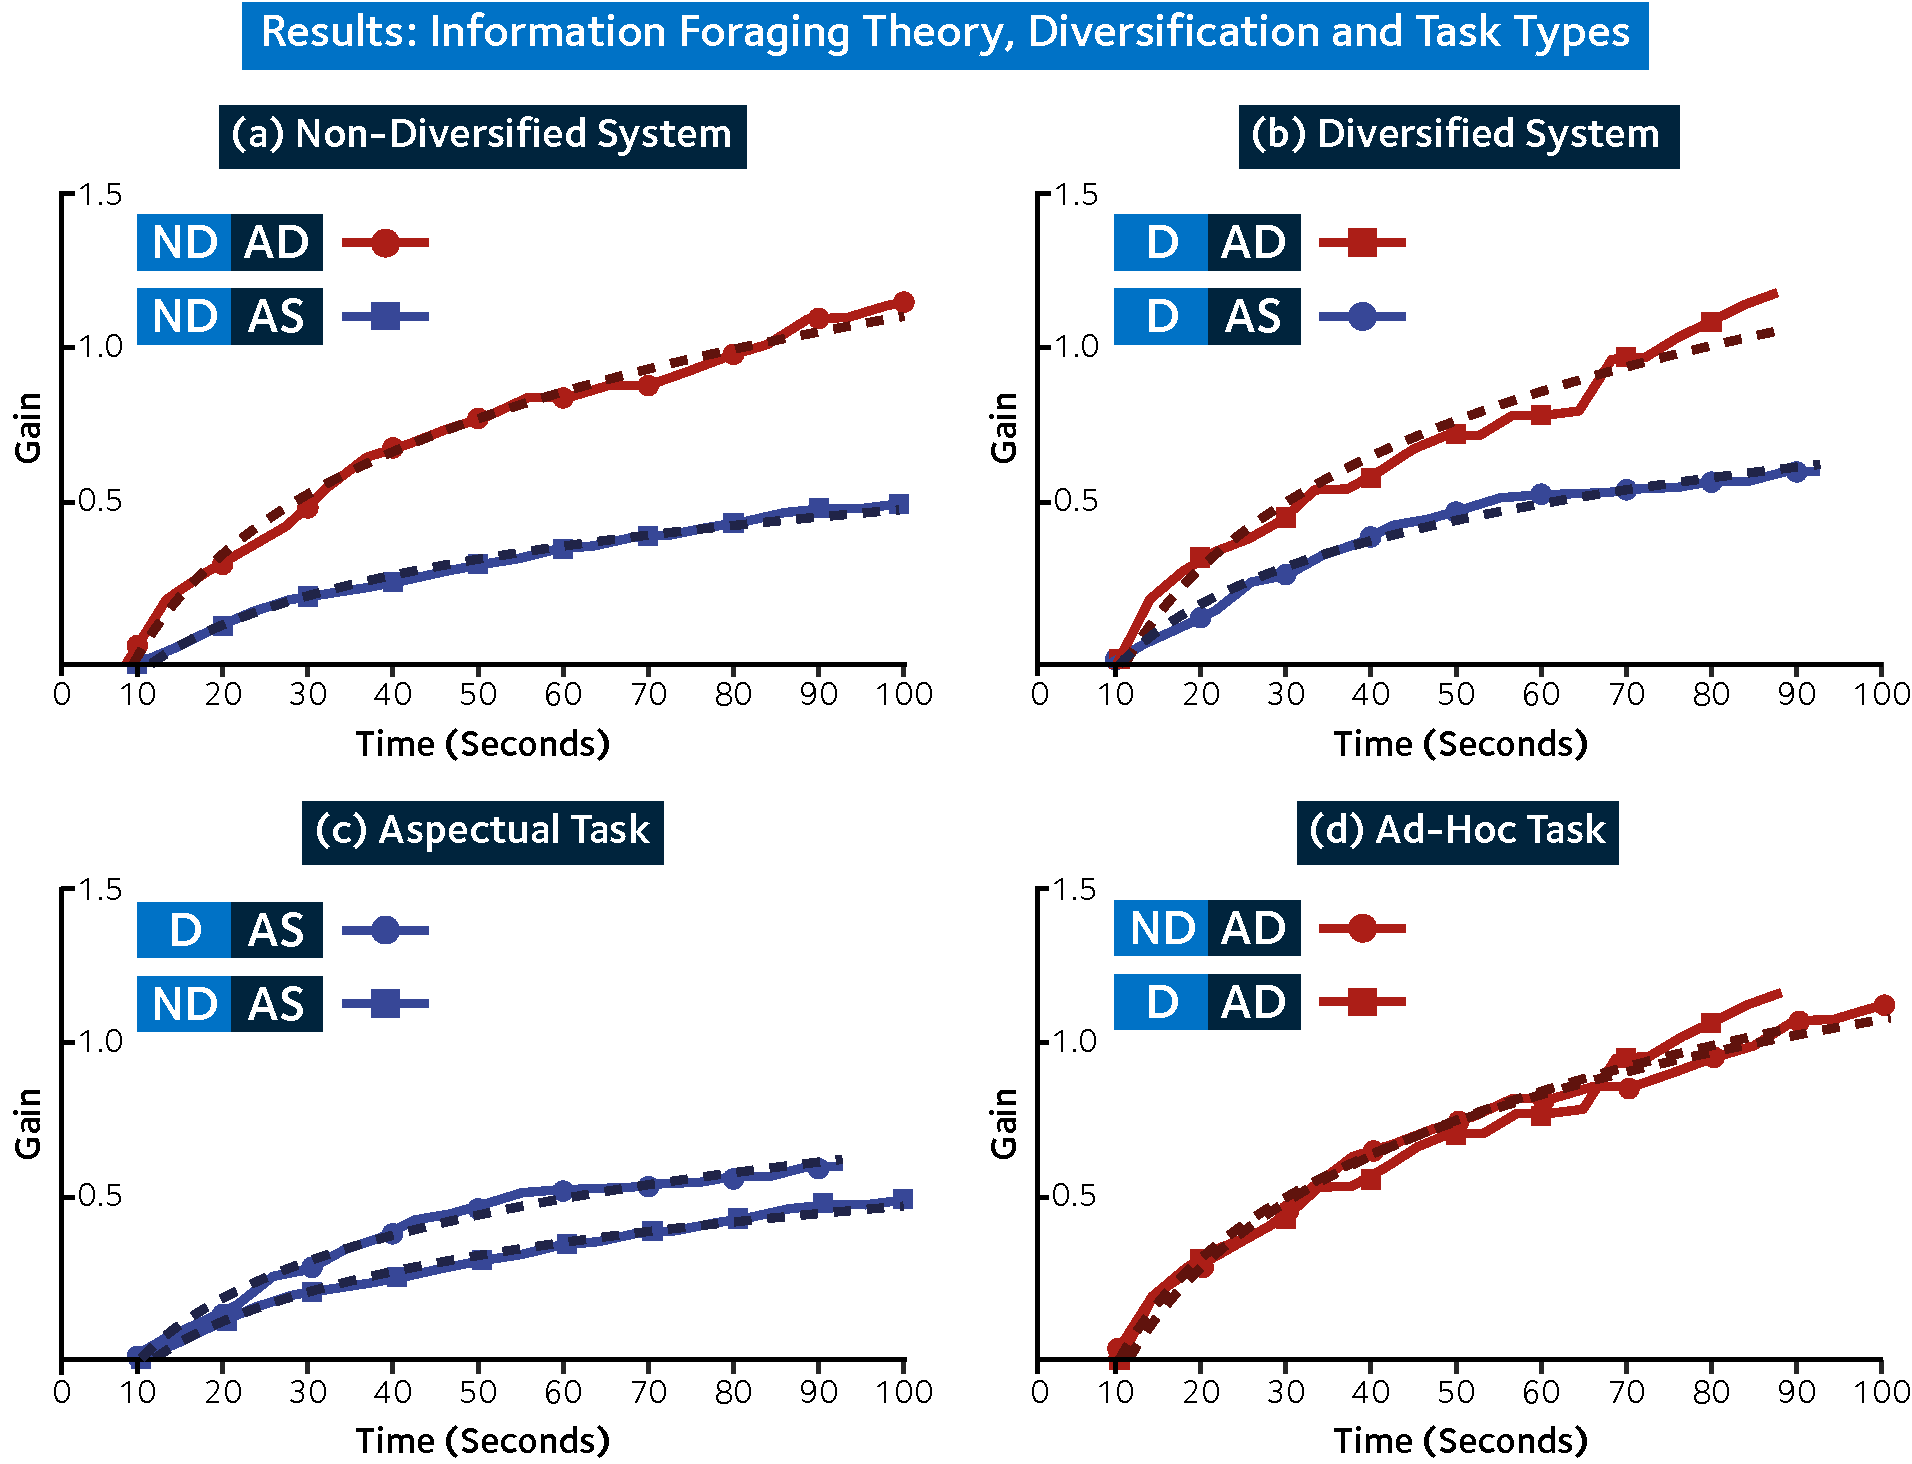
\includegraphics{figures/ch8-ift_empirical_plots.pdf}}
    \caption[\gls{acr:ift} and diversification: empirical results]{Plots illustrating the~\glsfirst{acr:cg} attained by subjects of the user study (on average), over the first 100 seconds of a search session. Shown are plots with the four different combinations of experimental condition trialled. Dashed lines represent fitted curves.}
    \label{fig:ift_empirical}
\end{figure}

To do so, we first fit a logarithmic function to each of the gain curves given time, such that: $gain = b \cdot log(time) - a$, as used by~\cite{athukorala2014ift}. Table~\ref{tbl:aspects_ift_fitting} presents the parameters and correlation co-efficients for fit ($r^2$) for each of the four experimental conditions. We could then calculate how many documents a subjects examined by drawing the tangent line to the estimated gain functions from the origin. This resulted in the predicted number of documents examined, which we see are in line with the actual number of documents examined. With respect to plot \emph{(b)}, we see that for diversified system \blueboxbold{D}, the theory, given their performance, suggests that subjects should examine more documents per query under the aspectual task \blueboxbold{AS} than when undertaking the ad-hoc task \blueboxbold{AD} (i.e. $4.98$ vs. $3.68$ for \blueboxbold{AS} and \blueboxbold{AD}, respectively). We observed that subjects examined $3.48$ and $3.02$ documents per query -- which follows a similar trend, but not to the same magnitude. Thus, this revises our expectations regarding how people would search differently between these tasks.

\begin{table}[t!]
    \caption[\gls{acr:ift} fitting parameters]{Fitting parameters for the gain curves illustrated in Figure~\ref{fig:ift_empirical}, over each of the four experimental conditions trialled. Also included are the estimations from the model of the predicted number of documents that subjects would examine, and the actual number from the empirical data.\vspace*{-3mm}}
    \label{tbl:aspects_ift_fitting}
    \renewcommand{\arraystretch}{1.8}
    \begin{center}
    \begin{tabulary}{\textwidth}{L{2.9cm}@{\CS}D{2.08cm}@{\CS}D{2.08cm}@{\CS}D{2.08cm}@{\CSDOUBLE}D{2.08cm}@{\CS}D{2.08cm}@{\CS}}
        
        & \multicolumn{3}{@{\hskip 0pt}c@{\CS}}{\textbf{Model Fitting Parameters}} & \multicolumn{2}{@{\hskip 0pt}c@{\CS}}{\textbf{Predictions}} \\
        
        \RS & \lbluecell\textbf{a} & \lbluecell\textbf{b} & \lbluecell\textbf{r\textsuperscript{2}} & \lbluecell\textbf{Pred. D.} & \lbluecell\textbf{Actual D.} \\
        
        \RS \lbluecell\textbf{ND-AD} & \cell -1.08 & \cell 0.48 & \cell 0.989 & \cell 3.68 & \cell 3.23 \\
        \RS \lbluecell\textbf{ND-AS} & \cell -0.57 & \cell 0.23 & \cell 0.987 & \cell 4.92 & \cell 3.65 \\
        \RS \lbluecell\textbf{D-AD} & \cell -1.22 & \cell 0.52 & \cell 0.959 & \cell 4.98 & \cell 3.48 \\
        \RS \lbluecell\textbf{D-AS} & \cell -0.68 & \cell 0.29 & \cell 0.985 & \cell 4.36 & \cell 3.02 \\
    \end{tabulary}
    \end{center}
    \vspace*{-5mm}
\end{table}

With respect to \darkblueboxbold{H1}, we see that the theory, given their performance, suggests that participants -- when undertaking the aspectual retrieval task -- would examine fewer documents per query when using the diversified system \blueboxbold{D} than when using the non-diversified system, \blueboxbold{ND} ($4.36$ vs. $4.92$). Again, we see that subjects examined $3.02$ and $3.65$ documents per query respectively, again following the same trend -- but not to the same magnitude. This post-hoc analysis has provided justification for some of our initial hypotheses regarding how search behaviour would change under the different experimental conditions. However, it has also led to us revising our expectations based upon the empirical data.

\vspace*{-6mm}
\subsection{Discussion}
This user study has investigated the effects of diversifying search results when searchers undertook complex search tasks, requiring one to learn about different aspects of a topic. To test the series of hypotheses, derived from~\gls{acr:ift} outlined in Section~\ref{sec:diversity:background:tasks:hypotheses}, we conducted a within-subjects user study, using:

\begin{itemize}
    \item{a non-diversified system \blueboxbold{ND}; versus}
    \item{a diversified system \blueboxbold{D}.}
\end{itemize}

These were tested over two different search tasks, where the task was set to either:

\begin{itemize}
    \item{ad-hoc topic retrieval \blueboxbold{AD}; or}
    \item{aspectual retrieval \blueboxbold{AS}.}
\end{itemize}

This led to four experimental conditions. Findings from the study lend evidence to broadly support our hypotheses. However, our results were not statistically significant. This was despite the face that there were significant differences in how the two systems performed. As an example, the diversified system \blueboxbold{D} returned a ranked list of results with a greater number of documents containing new, unseen entities than when compared to system \blueboxbold{ND}. Clearly, bigger differences need to be present before individuals can subjectively begin to report on whether they had a different experience, or be able to clearly consider what system they preferred. This is clear as the post-task and post-experiment surveys revealed no differences between conditions as to what was preferred.

However, in terms of performance, we found that subjects of the study, when using retrieval system \blueboxbold{D}, did perform better. More relevant documents were found, and more new entities were found. This suggests that that found out more about topics on retrieval system \blueboxbold{D}. After conducting a post-hoc analysis, we showed that the hypotheses posted given~\gls{acr:ift} were indeed sound, but revised our expectations on how subjects would behave when using retrieval system \blueboxbold{D}. That is, they would examine more documents per query, and thus issue fewer queries when undertaking the aspectual retrieval task, as opposed to there being no difference in performance. Again, we observed a trend to support the hypothesis. Encouragingly, our application of~\gls{acr:ift}, before and after the study, led to new insights into how behaviours are affected under the different conditions. This is a useful tool in developing, motivating and analysing search performance and behaviours. Counter to our intuition about how we \emph{believed} people would behave under these conditions, the theory provided more informed and accurate hypotheses.

In past work, many interface-based solutions were studied, where a few significant differences in behaviour were found when compared to a standard interface. Disappointingly, we also found that an algorithmic solution has very little impact or influence either, though there were trends which indicated that diversifying search results does indeed lead to better performance, greater awareness of the topic (even when not specifically instructed, i.e. \emph{find relevant only}), and fewer examinations of non-relevant items. Thus, we suggest from this study that diversification should be employed more widely -- in particular in the context of news search -- where bias is an issue, and diversification algorithms can present a broader overview of the aspects within a topic.

From this study, we now move towards examining in more detail the stopping behaviour of searchers through a simulated analysis. The next section of this chapter details the simulated study, grounded from interaction data extracted from this user study.

\section{Simulated Analysis}\label{sec:diversity:simulated}
From the user study, we now move a simulated analysis of searcher stopping behaviour and performance. In this section, we detail how stopping behaviour and performance vary when searchers are subjected to differing search systems (i.e. \blueboxbold{D} vs. \blueboxbold{ND}) and search tasks (i.e. \darkblueboxbold{AD} vs. \darkblueboxbold{AS}). These are again, like in Section~\ref{sec:snippets:simulations}, addressed in the context of the two high-level research questions. Considering each of the twelve result summary level stopping strategies enumerated in Chapter~\ref{chap:strategies}, how does each:

\begin{itemize}
    \item{\darkblueboxbold{HL-RQ3a} perform; and}
    \item{\darkblueboxbold{HL-RQ3b} approximate actual searcher stopping behaviour?}
\end{itemize}

In the remainder of this section, we discuss the specific details of our methodology (Section~\ref{sec:diversity:simulated:method}), discussing in particular how we instantiated the task goals for these experiments. We then move onto an examination of the results from our simulations (Section~\ref{sec:diversity:simulated:results}).

\subsection{Methodology}\label{sec:diversity:simulated:method}
This methodology section outlines the details specific to how we instantiated this set of simulations. One can assume that any components that are not discussed in this section were instantiated as shown in the general simulation methodology. The general methodology is presented in Section~\ref{sec:method:simulation} on page~\pageref{sec:method:simulation}.

Two of the key differences between the simulations reported in Chapter~\ref{chap:snippets} are the how we operationalise the underlying retrieval engine to support diversity, and the simulated searcher \emph{task goals}. These are discussed in Section~\ref{sec:diversity:simulated:method:probscosts} below, after which we outline the interaction costs and probabilities we extracted from the user study data reported above (Section~\ref{sec:diversity:simulated:method:probscosts}).

\subsubsection{Experimental System and Conditions}\label{sec:diversity:simulated:method:system}
The \simiir~framework was adapted to incorporate additional components, allowing the simulations to employ the use of the diversified system \blueboxbold{D}, as well as the standard BM25-based non-diversified system, \blueboxbold{ND}. This therefore allowed us to run simulations over the four experimental conditions trialled as discussed in Section~\ref{sec:diversity:users:method}. Results returned for systems \blueboxbold{D} and \blueboxbold{ND} were therefore identical to results returned to the real-world subjects of the user study.

The second major components of the \simiir~framework that we considered were the result summary and document decision makers. These components, discussed in Section~\ref{sec:method:simulation:grounding:judgements}, determine whether a result summary is considered attractive enough to click, and whether a document is relevant to the given~\gls{acr:trec} topic. For aspectual search tasks \darkblueboxbold{AS}, the focus is not to simply save relevant documents, but to save relevant documents containing at least one new aspect of the topic. We however decided to keep the decision makers the same for both search tasks, meaning that only the relevance to the topic was considered. We do however report results with aspectual measures, such as aspectual recall, in Section~\ref{sec:diversity:simulated:results}.

\subsubsection{Interaction Costs and Probabilities}\label{sec:diversity:simulated:method:probscosts}
Interaction log data from the associated user study was then taken and filtered by the four experimental conditions. Following the methodology outlined in Sections~\ref{sec:method:simulation:grounding:judgements} and~\ref{sec:method:simulation:grounding:costs}, we then extracted the different interaction probabilities and costs to ground our simulations.

Table~\ref{tbl:diversity_simulation_probcosts} presents said interaction probabilities and costs across the four experimental interfaces trialled. Included within the table are the interaction probabilities for clicking on result summaries (under the \genericblack{P(C)} grouping) and saving documents (under the \genericblack{P(S)} grouping). Also included are the five main interaction costs, presented under the \genericblack{Costs} grouping.

\blueboxheader{Task Goal}
Also included in Table~\ref{tbl:diversity_simulation_probcosts} is the task goal. In the user study, subjects were instructed to find and save a minimum of four useful documents pertaining to the~\gls{acr:trec} topic, as reported back in Section~\ref{sec:diversity:users:method:tasks}. Subjects across all four experimental interfaces saved on average $5.87$ documents, perhaps to hedge their bets in the eventuality that certain saved documents turned out to not be useful after all. These values can be found in the \genericblack{\#Saved} row in Table~\ref{tbl:aspectual_combo_beperftime} on page~\pageref{tbl:aspectual_combo_beperftime}. As such, simulated searchers were given a goal of finding \emph{six} useful documents to mirror the average saved by their real-world counterparts.

\blueboxheader{Session Timeout}
A session timeout was also provided such that if simulated searchers failed to find the minimum of six useful documents, the timeout would prevent the simulation from getting stuck, with the simulated searchers browsing to wholly unrealistic depths. Again referring to Table~\ref{tbl:aspectual_combo_beperftime} on page~\pageref{tbl:aspectual_combo_beperftime}, the mean total session time (reported on row \genericblack{Total Session}) was reported to be $438.47$ seconds on average across all four experimental conditions. With a large variance in time, we set a hard simulated search session time limit of $500$ seconds (equating to the upper side of the standard deviation), to grant sufficient time for searchers to find the six required documents, yet not permitting runaway behaviours.

Simulations of interaction when considering aspectual retrieval tasks have to the best of our knowledge not been performed before. A majority of prior work purely considers ad-hoc retrieval, given that this is a relatively straightforward search task to model. We therefore believe that the assumptions made for these simulations of interaction provides a reasonable approximation for how real-world searchers actually performed and behaved, and leaves scope for development of these simulations in future work. We leave discussion on these assumptions and potential issues that may arise from them to Chapter~\ref{chap:conclusions}.

\begin{table}[t!]
    \caption[Simulations interaction probabilities and costs (diversification)]{Summary table of the different interaction costs (in seconds) and probabilities, with \genericblack{P(C)} denoting the probability of a click, and \genericblack{P(S)} denoting the probability of saving a document (considering it relevant). Values are reported across the four experimental conditions trialled. Refer to Sections~\ref{sec:method:simulation:grounding:costs} and~\ref{sec:method:simulation:grounding:judgements} respectively for further information on how the costs and probabilities were derived. All data in this table is attained from interaction data extracted from the user study reported in Section~\ref{sec:diversity:users}.}
    \label{tbl:diversity_simulation_probcosts}
    \renewcommand{\arraystretch}{1.8}
    \begin{center}
    \begin{tabulary}{\textwidth}{L{0.4cm}@{\CS}L{3.2cm}@{\CS}D{2.5cm}@{\CS}D{2.5cm}@{\CS}D{2.5cm}@{\CS}D{2.5cm}@{\CS}}

        & & \lbluecell \textbf{D-AS} & \lbluecell \textbf{ND-AS} & \lbluecell \textbf{D-AD} & \lbluecell \textbf{ND-AD} \\

        \RS \multirow{2}{*}{\rotatebox{90}{\hspace*{-2mm}\textbf{P(C)}}} & \lbluecell\textbf{P(C|R)} & \cell \small{0.27} & \cell \small{0.30} & \cell \small{0.25} & \cell \small{0.31}\\
        \RS & \lbluecell\textbf{P(C|N)} & \cell \small{0.13} & \cell \small{0.18} & \cell \small{0.13} & \cell \small{0.17}\\
        
        \RS\RS\RS \multirow{2}{*}{\rotatebox{90}{\hspace*{-2mm}\textbf{P(S)}}} & \lbluecell\textbf{P(S|R)} & \cell \small{0.78} & \cell \small{0.63} & \cell \small{0.74} & \cell \small{0.67}\\
        \RS & \lbluecell\textbf{P(S|N)} & \cell \small{0.59} & \cell \small{0.61} & \cell \small{0.65} & \cell \small{0.65}\\
        
        \RS\RS\RS \multirow{5}{*}{\rotatebox{90}{\hspace*{-5.5mm}\textbf{Costs (in seconds)}}} & \lbluecell\textbf{Query} & \cell \small{8.80} & \cell \small{9.99} & \cell \small{9.69} & \cell \small{8.69}\\
        \RS & \lbluecell\textbf{\gls{acr:serp}} & \cell \small{5.92} & \cell \small{6.29} & \cell \small{6.36} & \cell \small{5.79}\\
        \RS & \lbluecell\textbf{Result Summary} & \cell \small{1.59} & \cell \small{1.75} & \cell \small{1.71} & \cell \small{1.71}\\
        \RS & \lbluecell\textbf{Document} & \cell \small{15.97} & \cell \small{13.03} & \cell \small{13.66} & \cell \small{15.09}\\
        \RS & \lbluecell\textbf{Save} & \cell \small{1.73} & \cell \small{1.78} & \cell \small{1.58} & \cell \small{1.68}\\
        
        \RS\RS\RS & \lbluecell\textbf{Task Goal} & \multicolumn{4}{@{\hskip 0pt}c@{\CS}}{\cell Find 6 relevant (refer to Section~\ref{sec:diversity:simulated:method:probscosts})}\\
        \RS & \lbluecell\textbf{Session Timeout} & \multicolumn{4}{@{\hskip 0pt}c@{\CS}}{\cell 500 seconds (refer to Section~\ref{sec:diversity:simulated:method:probscosts})}\\
        
    \end{tabulary}
    \end{center}
\end{table}

\subsection{Results}\label{sec:diversity:simulated:results}
We now report the results of our simulations of interaction, under different search tasks and goals. Like our findings in Chapter~\ref{chap:snippets}, we discuss our findings over two subsections, considering:

\begin{itemize}
    \item{the \emph{performance} runs (Section~\ref{sec:diversity:simulated:results:perf}), where we discuss the highest levels of performance attained by simulated searchers under different \emph{what-if} scenarios; and}
    \item{the \emph{comparison} runs (Section~\ref{sec:diversity:simulated:results:comparisons}), where we provide results of the simulations that were directly compared to actual mean searcher behaviours.}
\end{itemize}

Both of these sections provide an answer for high-level research questions \darkblueboxbold{HL-RQ3a} and \darkblueboxbold{HL-RQ3b} respectively, this time under the context of varying search tasks and goals.

\blueboxheader{Significance Testing}
We once again employ significance testing to determine whether the performance of a result summary level stopping strategy was significantly different from others. All tests in this section utilise the two-tailed Student's t-test, where $\alpha=0.05$. We compare the best performing or approximating stopping strategies against the other eleven. Here, we are interested in \emph{statistical non-significance} (i.e. $\alpha > 0.05$), meaning that compared stopping strategies are \emph{similar} to one another in terms of performance or approximations.

\subsubsection{Performance}\label{sec:diversity:simulated:results:perf}
\vspace*{-3mm}
Before reporting on the performance of each stopping strategy across our performance \emph{(what-if)} simulations, we must first determine whether querying strategy \blueboxbold{QS13} delivers queries of expected performance across systems \blueboxbold{ND} (non-diversified) and \blueboxbold{D} (diversified). From the performance across the two systems when constituting part of the user study (as shown in Table~\ref{tbl:aspects_system_comparison}), we observed significant differences in terms of precision, $\alpha DCG$ and $AR$. Results from the user study showed consistently higher levels of $\alpha DCG$ and $AR$ were observed over system \blueboxbold{D}, a result that was in line with expectations.

Table~\ref{tbl:ch8_sim_queryperf} reports various precision, $\alpha DCG$ and $AR$ for queries generated by querying strategy \blueboxbold{QS13}. Across both systems \blueboxbold{ND} and \blueboxbold{D}, measures ($\pm$ standard deviations) are shown across all three stopping strategies, including \blueboxbold{QS13} and constituent querying strategies \blueboxbold{QS1} (single term, poor queries) and \blueboxbold{QS3} (three term, good queries). Queries were extracted from the simulated interaction logs, with a total of $213$ unique queries being extracted. Queries were then categorised depending upon their term length, allowing us to deduce measures for each individual querying strategy.

\begin{table}[t!]
    \caption[Performance of querying strategies across systems \blueboxbold{ND} and \blueboxbold{D}]{Mean performance values ($\pm$ standard deviations) of all generated queries issued for performance runs. Included are \emph{P@k}, $\alpha$\emph{DCG@k} and \emph{AR@k} values, incorporating aspectual retrieval measures. Values are reported across both the non-diversified (\blueboxbold{ND}) and diversified (\blueboxbold{D}) systems. Note the increasing trends in performance across all measures as \blueboxbold{QS1} $\rightarrow$ \blueboxbold{QS3}, as well as the improved performance for diversification measures over system \blueboxbold{D}.}
    \label{tbl:ch8_sim_queryperf}
    \renewcommand{\arraystretch}{1.8}
    \begin{center}
    \begin{tabulary}{\textwidth}{L{2.1cm}@{\CS}D{1.8cm}@{\CS}D{1.8cm}@{\CS}D{1.8cm}@{\CSONEHALF}D{1.8cm}@{\CS}D{1.8cm}@{\CS}D{1.8cm}@{\CS}}
        
        & \multicolumn{3}{@{\hskip 0pt}c@{\CSONEHALF}}{\dbluecell\small\textbf{ND}} & \multicolumn{3}{@{\hskip 0pt}c@{\CS}}{\dbluecell\small\textbf{D}} \\
        \RS & \lbluecell\textbf{QS1} & \lbluecell\textbf{QS13} & \lbluecell\textbf{QS3} & \lbluecell\textbf{QS1} & \lbluecell\textbf{QS13} & \lbluecell\textbf{QS3} \\
        
        \RS\lbluecell\textbf{P@1} & \cell\footnotesize 0.04 $\pm$ 0.20 & \cell\footnotesize 0.18 $\pm$ 0.39 & \cell\footnotesize 0.23 $\pm$ 0.42 & \cell\footnotesize 0.04 $\pm$ 0.20 & \cell\footnotesize 0.19 $\pm$ 0.39 & \cell\footnotesize 0.23 $\pm$ 0.43 \\
        \RS\lbluecell\textbf{P@5} & \cell\footnotesize 0.02 $\pm$ 0.07 & \cell\footnotesize 0.14 $\pm$ 0.21 & \cell\footnotesize 0.18 $\pm$ 0.23 & \cell\footnotesize 0.05 $\pm$ 0.16 & \cell\footnotesize 0.18 $\pm$ 0.26 & \cell\footnotesize 0.22 $\pm$ 0.28 \\
        \RS\lbluecell\textbf{P@10} & \cell\footnotesize 0.02 $\pm$ 0.06 & \cell\footnotesize 0.11 $\pm$ 0.18 & \cell\footnotesize 0.15 $\pm$ 0.19 & \cell\footnotesize 0.03 $\pm$ 0.10 & \cell\footnotesize 0.14 $\pm$ 0.20 & \cell\footnotesize 0.17 $\pm$ 0.21 \\

        \RS\RS\RS\lbluecell\textbf{$\alpha$DCG@5} & \cell\footnotesize 0.00 $\pm$ 0.00 & \cell\footnotesize 0.01 $\pm$ 0.03 & \cell\footnotesize 0.02 $\pm$ 0.03 & \cell\footnotesize 0.00 $\pm$ 0.00 & \cell\footnotesize 0.02 $\pm$ 0.04 & \cell\footnotesize 0.02 $\pm$ 0.04 \\
        \RS\lbluecell\textbf{$\alpha$DCG@10} & \cell\footnotesize 0.00 $\pm$ 0.00 & \cell\footnotesize 0.01 $\pm$ 0.03 & \cell\footnotesize 0.02 $\pm$ 0.03 & \cell\footnotesize 0.00 $\pm$ 0.01 & \cell\footnotesize 0.02 $\pm$ 0.04 & \cell\footnotesize 0.03 $\pm$ 0.05 \\

        \RS\RS\RS\lbluecell\textbf{AR@5} & \cell\footnotesize 0.01 $\pm$ 0.04 & \cell\footnotesize 0.30 $\pm$ 0.87 & \cell\footnotesize 0.40 $\pm$ 0.98 & \cell\footnotesize 0.05 $\pm$ 0.24 & \cell\footnotesize 0.51 $\pm$ 1.25 & \cell\footnotesize 0.65 $\pm$ 1.40 \\
        \RS\lbluecell\textbf{AR@10} & \cell\footnotesize 0.01 $\pm$ 0.04 & \cell\footnotesize 0.20 $\pm$ 0.51 & \cell\footnotesize 0.27 $\pm$ 0.58 & \cell\footnotesize 0.03 $\pm$ 0.13 & \cell\footnotesize 0.30 $\pm$ 0.69 & \cell\footnotesize 0.38 $\pm$ 0.77 \\
    \end{tabulary}
    \end{center}
\end{table}

Examining at Table~\ref{tbl:ch8_sim_queryperf}, we see that as we move from \blueboxbold{QS1} to \blueboxbold{QS3}, a consistent improvement in precision can be observed. Again, this findings is in line with intuition. Interleaved querying strategy \blueboxbold{QS13} delivers intermediary performance on average. This shows that when interleaving single then tri term queries offers good levels of mean precision. When we turn our attention to aspectual measures, we again see the general trend of performance improvements as we tend from \blueboxbold{QS1} to \blueboxbold{QS3}. Furthermore, when contrasting between systems \blueboxbold{ND} and \blueboxbold{D}, we once again see jumps in performance. For example, $AR@10$ is reported as $0.27\pm0.58$ for system \blueboxbold{ND}, with $0.38\pm0.77$ for system \blueboxbold{D}. This jump in mean aspectual recall demonstrates that once again the diversification algorithm presented in Figure/Algorithm~\ref{alg:diversifying} does indeed return a greater number of unique aspects for each individual topic trialled.

Results from Table~\ref{tbl:ch8_sim_queryperf} therefore provide us with confidence that the two systems were indeed working as intended, yielding queries that performed in line with our intuition, and offered similar trends in performance compared to those issued by the real-world subjects of the user study. We also gain confidence in knowing that interleaved querying strategy \blueboxbold{QS13} also offers improvements in aspectual measures compared to \blueboxbold{QS1}. As such, this should be later reflected in our examination of the what-if experiments when we consider aspectual measures.

Satisfied with the performance of the generated queries, we now turn our attention to an examination of the individual result summary level stopping strategies. Like our reporting in Section~\ref{sec:snippets:simulations:results:perf}, we consider results primarily from the perspective of \darkblueboxbold{HL-RQ3a}, which requires an examination of the performance of each stopping strategy. Before this, we consider the general trends that we observed across the performance simulations, examining whether these trends are consistent across the experimental conditions trialled.

Figure~\ref{fig:ch8_sim_perf_plots} presents twelve individual plots, one per result summary level stopping strategy. These plots represent the mean levels of performance attained over each experimental condition (of either \dualbluebox{D}{AS}, \dualbluebox{ND}{AS}, \dualbluebox{D}{AD} or \dualbluebox{ND}{AD}) at varying depths per query, averaged over the five individual topics and 50 individual trials. The mean depth per query is represented along each $x$ axis, with the performance attained (represented as~\gls{acr:cg}) represented along the $y$ axes. Although strategies such as \blueboxbold{SS3-NC} allowed simulated searchers to browse to depths greater than 25 on average, all plots were cut at this depth for consistency, and to highlight what occurs at lower depths per query. Each point on the respective lines for each condition represents one of the stopping threshold values used for each stopping strategy, as reported in Table~\ref{tbl:stopping_thresholds}.

General trends across mean depths per query can be observed in each of the twelve plots in Figure~\ref{fig:ch8_sim_perf_plots}. We can see across a majority of stopping strategies and experimental conditions that as the mean depth per query increases, simulated searchers attain greater of levels of~\gls{acr:cg} on average before a peak point of~\gls{acr:cg} attainment is reached. After this point, as searchers traverse result lists to greater depths, the mean level of~\gls{acr:cg} begins to diminish. Peaks can be more profound in some stopping strategies (e.g. \blueboxbold{SS1-FIX} and \blueboxbold{SS5-COMB}) than with others (e.g. \blueboxbold{SS4-SAT}). This trend can be observed across all four experimental conditions, where all four start at very similar levels of mean~\gls{acr:cg} across shallow mean depths per query, before gaps begin to emerge between them. Indeed, it can be observed across the twelve plots that condition \dualbluebox{D}{AS} consistently offers the best approximations across nearly all depths per query reported. This condition is very closely followed by \dualbluebox{D}{AD}, with slightly lower mean levels of~\gls{acr:cg}. Interestingly, we then observe a gap between these two conditions, and the remaining two conditions, \dualbluebox{ND}{AS} and \dualbluebox{ND}{AD}. This gap is largely present amongst all twelve stopping strategies, and is more profound in stopping strategies that offer higher mean levels of~\gls{acr:cg}. This is especially true after peak~\gls{acr:cg} has been reached, and the mean depth per query begins to increase. The gaps between conditions clearly demonstrate a difference in performance between systems \blueboxbold{D} and \blueboxbold{ND}, with system \blueboxbold{D} consistently offering improved mean levels of~\gls{acr:cg}. Interestingly however, gaps between tasks \darkblueboxbold{AD} and \darkblueboxbold{AS} are less profound, with negligible differences observed from examination of the twelve plots.

\begin{figure}[p!]
    \centering
    \resizebox{1\hsize}{!}{
    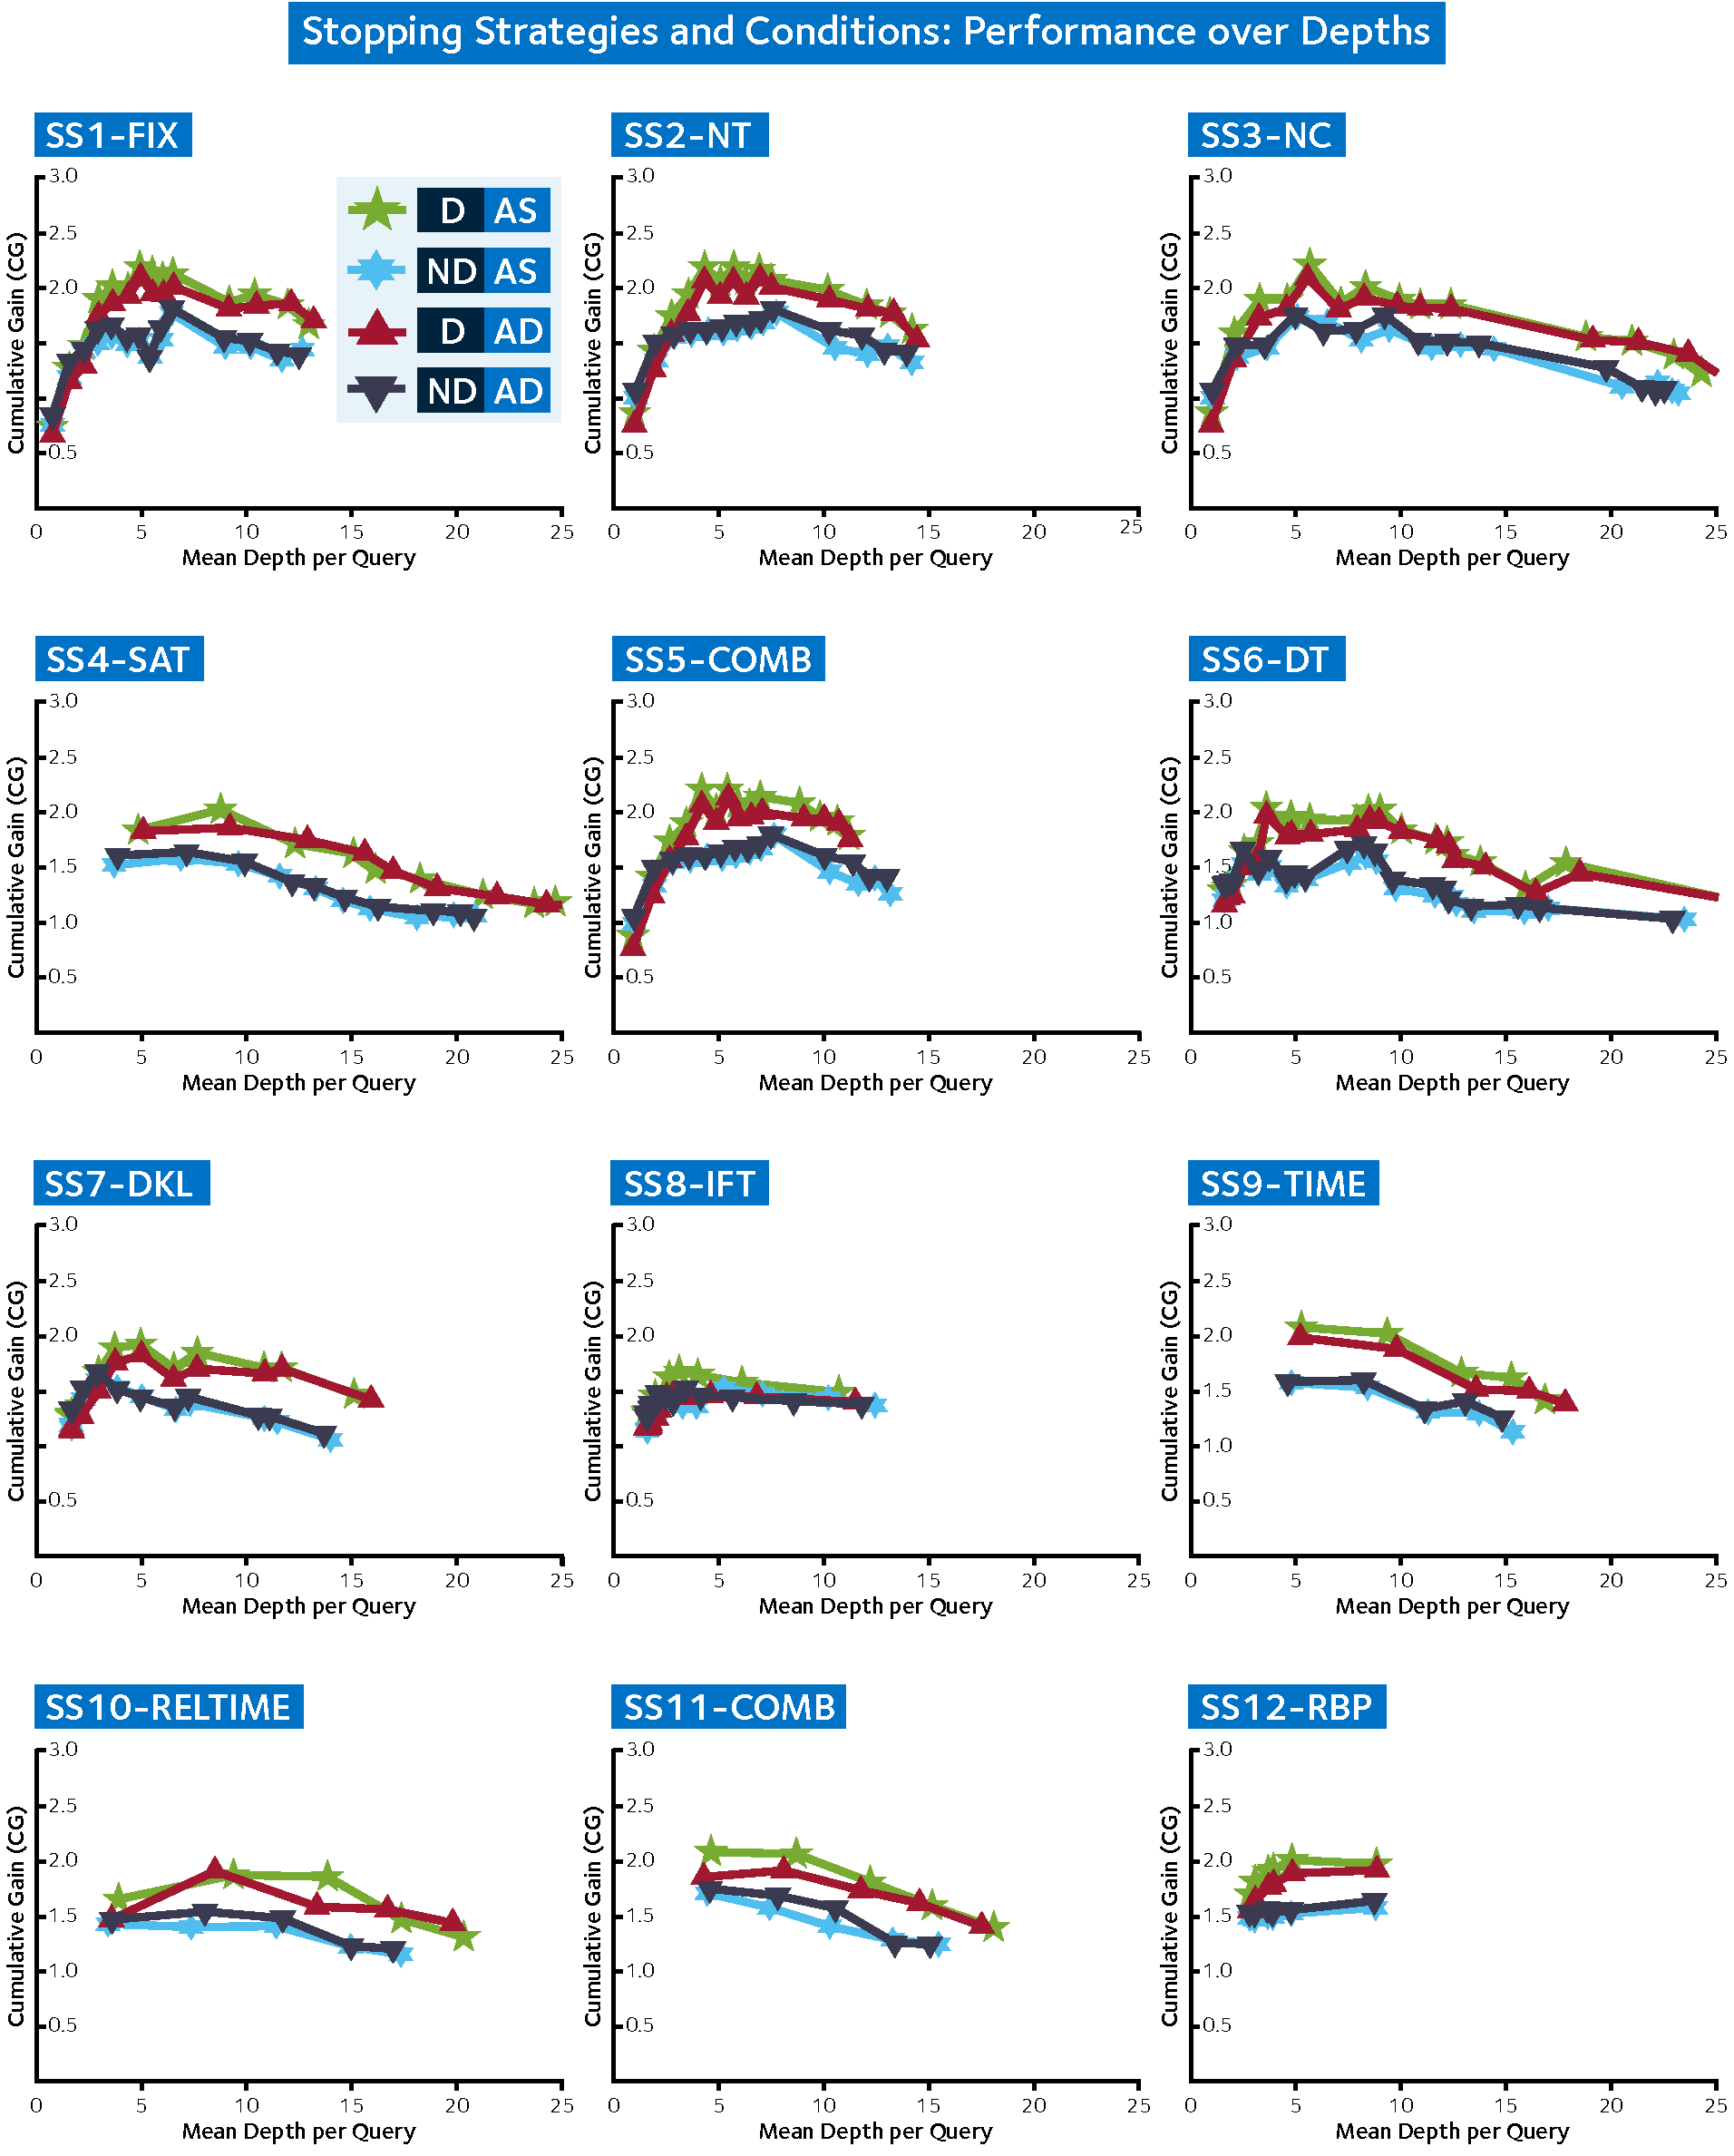
\includegraphics{figures/ch8-perf_plots.pdf}}
    \caption[Performance plots (diversification)]{Plots showing the varying levels of performance, measured in~\gls{acr:cg}, over the mean depth per query. Each result summary stopping strategy is shown on an individual plot, with each of the four experimental conditions shown within each plot. The depth per query reported on each \emph{x} axis is cut at 25 to allow for an easier comparison between different stopping strategies.}
    \label{fig:ch8_sim_perf_plots}
\end{figure}

While the plots in Figure~\ref{fig:ch8_sim_perf_plots} present the general trends in performance across mean depths per query, Table~\ref{tbl:ch8_sim_perf} reports on the \emph{highest level of~\gls{acr:cg}} attained by each result summary level stopping strategy, across the four experimental conditions trialled. The values in Table~\ref{tbl:ch8_sim_perf} therefore correspond to the peaks shown in each of the plots in Figure~\ref{fig:ch8_sim_perf_plots}. For each stopping strategy and condition, we report: the highest level of~\gls{acr:cg} attained \genericblack{(CG)}; the mean depth per qury at which this value was reached \genericblack{(DQ)}; and the stopping threshold value(s) that were used to attain this value \genericblack{(x\textsubscript{n})}. \darkbluebox{Highlighted} are the stopping strategies that yielded the highest mean level of~\gls{acr:cg}, with the highest value demonstrated for each condition. For conditions \dualbluebox{D}{AS}, \dualbluebox{ND}{AS} and \dualbluebox{D}{AD}, combination stopping strategy \blueboxbold{SS5-COMB} attains the highest mean level of~\gls{acr:cg}, with values $2.21$, $1.79$ and $2.13$ reached for the aforementioned condition, respectively. As these levels of~\gls{acr:cg} are reached under a combination strategy, values $x_2=5$ and $x_4=3$, $x_2=10$ and $x_4=6$, and $x_2=7$ and $x_4=3$ were used to attain these values for conditions \dualbluebox{D}{AS}, \dualbluebox{ND}{AS} and \dualbluebox{D}{AD}, respectively. This means that under condition \dualbluebox{D}{AS}, a searcher would examine a total of five non-relevant documents or save three relevant documents per query before stopping -- whatever occurred first. Interestingly, our fixed-depth, baseline stopping strategy \blueboxbold{SS1-FIX} reaches the highest level of~\gls{acr:cg} for condition \dualbluebox{ND}{AD}, at $1.81$. \blueboxbold{SS5-COMB} is however very close behind, with a mean~\gls{acr:cg} of $1.80$ reported. Like results in Section~\ref{sec:snippets:simulations:results:perf}, this again demonstrates that a fixed-depth strategy can be hard to beat in terms of attaining a high level of~\gls{acr:cg}.

Indeed, it should be noted that several stopping strategies reported maximum levels of~\gls{acr:cg} close to the absolute maximum observed:

\begin{itemize}
    
    \item{\blueboxbold{SS2-NT} and \blueboxbold{SS3-NC}, the frustration stopping strategies (considering total and contiguous non-relevance);}
    \item{\blueboxbold{SS4-SAT}, the satiation-based stopping strategy;}
    \item{\blueboxbold{SS9-TIME}, the time-based strategy; and}
    \item{\blueboxbold{SS11-COMB}, the patch-based combination strategy}
    
\end{itemize}

\noindent
all report good levels of performance across the four conditions. For \blueboxbold{SS5-COMB}, the relatively low mean depths per query at which the greatest level of~\gls{acr:cg} was reached also demonstrates that the combination strategy was particularly robust at detecting a query of poor performance, and subsequently stopping at shallower depths (thus saving the simulated searcher's time). Taking this further, an interesting trend that was initially observed in Figure~\ref{fig:ch8_sim_perf_plots} shows that peak~\gls{acr:cg} is attained at generally shallower mean depths per query under tasks using system \blueboxbold{D} than when compared to system \blueboxbold{ND}.

\begin{table}[p!]
    \caption[Maximum CG from diversification performance runs]{Results from the simulated what-if simulated performance runs, showing the highest levels of~\gls{acr:cg} attained for each result summary level stopping strategy trialled (grouped by their type). \emph{x\textsubscript{n}} denotes the parameter threshold(s), with \emph{DQ} denoting the depth per query at which the greatest~\gls{acr:cg} value was attained at. For each condition, the stopping strategy which attained the highest level of~\gls{acr:cg} is \darkbluebox{highlighted}. \cellbluebox{Light blue} highlighting denotes \emph{no significant difference} from the best performing strategy, with no highlighting denoting a significant difference at $\alpha$\emph{=0.05.} For combination thresholds, \emph{x\textsubscript{2},x\textsubscript{4}} are presented for \blueboxbold{SS5-COMB}, with \emph{x\textsubscript{10},x\textsubscript{4}} for \blueboxbold{SS11-COMB}.}
    \label{tbl:ch8_sim_perf}
    \renewcommand{\arraystretch}{1.8}
    \begin{center}
        \begin{tabulary}{\textwidth}{L{0.00cm}@{\CS}L{1cm}@{\CS}D{0.64cm}@{\CS}D{0.64cm}@{\CS}D{0.64cm}@{\CSONEHALF}D{0.64cm}@{\CS}D{0.64cm}@{\CS}D{0.64cm}@{\CSONEHALF}D{0.64cm}@{\CS}D{0.64cm}@{\CS}D{0.64cm}@{\CSONEHALF}D{0.64cm}@{\CS}D{0.64cm}@{\CS}D{0.64cm}@{\CS}}
            
            & & \multicolumn{3}{@{\hskip 0pt}c@{\CSONEHALF}}{\dbluecell\small\textbf{D-AS}} & \multicolumn{3}{@{\hskip 0pt}c@{\CSONEHALF}}{\dbluecell\small\textbf{ND-AS}} & \multicolumn{3}{@{\hskip 0pt}c@{\CSONEHALF}}{\dbluecell\small\textbf{D-AD}} & \multicolumn{3}{@{\hskip 0pt}c@{\CS}}{\dbluecell\small\textbf{ND-AD}}\\
            
            \RS & & \lbluecell\small\textbf{x\textsubscript{n}} & \lbluecell\small\textbf{DQ} & \lbluecell\small\textbf{CG} & \lbluecell\small\textbf{x\textsubscript{n}} & \lbluecell\small\textbf{DQ} & \lbluecell\small\textbf{CG} & \lbluecell\small\textbf{x\textsubscript{n}} & \lbluecell\small\textbf{DQ} & \lbluecell\small\textbf{CG} & \lbluecell\small\textbf{x\textsubscript{n}} & \lbluecell\small\textbf{DQ} & \lbluecell\small\textbf{CG} \\
            
            \RS \multirow{1}{*}{\hspace*{-2mm}\rotatebox{90}{\hspace*{-1mm}\small\textbf{FIX}}} & \lbluecell\small\textbf{SS1}  & \cell \small \hspace*{-1mm} 7 & \cell \small \hspace*{-1mm} 4.95 & \cell \hspace*{-1mm} \small 2.19 & \cell \small \hspace*{-1mm} 10 & \cell \small \hspace*{-1mm} 6.45 & \cell \hspace*{-1mm} \small 1.77 & \cell \small \hspace*{-1mm} 7 & \cell \small \hspace*{-1mm} 4.99 & \cell \hspace*{-1mm} \small 2.09 & \dbluecell \small \hspace*{-1mm} 10 & \dbluecell \small \hspace*{-1mm} 6.47 & \dbluecell \hspace*{-1mm} \small 1.81 \\
            
            \RS\RS\RS \multirow{2}{*}{\hspace*{-2mm}\rotatebox{90}{\hspace*{-3mm}\small\textbf{FRUS}}} & \lbluecell\small\textbf{SS2} & \cell \small \hspace*{-1mm} 5 & \cell \small \hspace*{-1mm} 4.29 & \cell \hspace*{-1mm} \small 2.18 & \cell \small \hspace*{-1mm} 10 & \cell \small \hspace*{-1mm} 7.71 & \cell \hspace*{-1mm} \small 1.76 & \cell \small \hspace*{-1mm} 9 & \cell \small \hspace*{-1mm} 6.93 & \cell \hspace*{-1mm} \small 2.08 & \cell \small \hspace*{-1mm} 10 & \cell \small \hspace*{-1mm} 7.55 & \cell \hspace*{-1mm} \small 1.80 \\
            
            \RS & \lbluecell\small\textbf{SS3} & \cell \small \hspace*{-1mm} 5 & \cell \small \hspace*{-1mm} 5.64 & \cell \hspace*{-1mm} \small 2.20 & \cell \small \hspace*{-1mm} 4 & \cell \small \hspace*{-1mm} 5.03 & \cell \hspace*{-1mm} \small 1.73 & \cell \small \hspace*{-1mm} 5 & \cell \small \hspace*{-1mm} 5.52 & \cell \hspace*{-1mm} \small 2.08 & \cell \small \hspace*{-1mm} 4 & \cell \small \hspace*{-1mm} 4.93 & \cell \hspace*{-1mm} \small 1.74 \\
            
            \RS\RS\RS \multirow{1}{*}{\hspace*{-2mm}\rotatebox{90}{\small\textbf{SAT}}} & \lbluecell\small\textbf{SS4} & \cell \small \hspace*{-1mm} 2 & \cell \small \hspace*{-1mm} 8.77 & \cell \hspace*{-1mm} \small 2.01 & \cell \small \hspace*{-1mm} 2 & \cell \small \hspace*{-1mm} 6.87 & \cell \hspace*{-1mm} \small 1.57 & \cell \small \hspace*{-1mm} 2 & \cell \small \hspace*{-1mm} 9.21 & \cell \hspace*{-1mm} \small 1.85 & \cell \small \hspace*{-1mm} 2 & \cell \small \hspace*{-1mm} 7.15 & \cell \hspace*{-1mm} \small 1.63 \\
            
            \RS\RS\RS \multirow{1}{*}{\hspace*{-2mm}\rotatebox{90}{\small\textbf{COM}}} & \lbluecell\small\textbf{SS5} & \dbluecell \small \hspace*{-1mm} 5,3 & \dbluecell \small \hspace*{-1mm} 4.21 & \dbluecell \hspace*{-1mm} \small 2.21 & \dbluecell \small \hspace*{-1mm} 10,6 & \dbluecell \small \hspace*{-1mm} 7.65 & \dbluecell \hspace*{-1mm} \small 1.79 & \dbluecell \small \hspace*{-1mm} 7,3 & \dbluecell \small \hspace*{-1mm} 5.47 & \dbluecell \hspace*{-1mm} \small 2.13 & \cell \small \hspace*{-1mm} 10,6 & \cell \small \hspace*{-1mm} 7.50 & \cell \hspace*{-1mm} \small 1.80 \\
            
            \RS\RS\RS \multirow{2}{*}{\hspace*{-2mm}\rotatebox{90}{\small\textbf{DIFF}}} & \lbluecell\small\textbf{SS6} & \cell \small \hspace*{-1mm} 0.30 & \cell \small \hspace*{-1mm} 3.58 & \cell \hspace*{-1mm} \small 2.02 & \cell \small \hspace*{-1mm} 0.55 & \cell \small \hspace*{-1mm} 8.29 & \cell \hspace*{-1mm} \small 1.58 & \cell \small \hspace*{-1mm} 0.30 & \cell \small \hspace*{-1mm} 3.60 & \cell \hspace*{-1mm} \small 1.95 & \cell \small \hspace*{-1mm} 0.55 & \cell \small \hspace*{-1mm} 8.22 & \cell \hspace*{-1mm} \small 1.70 \\
            
            \RS & \lbluecell\small\textbf{SS7} & \cell \small \hspace*{-1mm} 5.5 & \cell \small \hspace*{-1mm} 4.91 & \cell \hspace*{-1mm} \small 1.92 & \cell \small \hspace*{-1mm} 6.5 & \cell \small \hspace*{-1mm} 2.87 & \cell \hspace*{-1mm} \small 1.59 & \cell \small \hspace*{-1mm} 5.5 & \cell \small \hspace*{-1mm} 4.95 & \cell \hspace*{-1mm} \small 1.82 & \cell \small \hspace*{-1mm} 6.5 & \cell \small \hspace*{-1mm} 2.86 & \cell \hspace*{-1mm} \small 1.66 \\
            
            \RS\RS\RS \multirow{1}{*}{\hspace*{-2mm}\rotatebox{90}{\small\textbf{IFT}}} & \lbluecell\small\textbf{SS8} & \small \hspace*{-2.5mm} 0.008 & \small \hspace*{-1mm} 3.18 & \hspace*{-1mm} \small 1.68 & \cell \small \hspace*{-2.5mm} 0.008 & \cell \small \hspace*{-1mm} 5.30 & \cell \hspace*{-1mm} \small 1.53 & \small \hspace*{-2.5mm} 0.006 & \small \hspace*{-1mm} 4.68 & \hspace*{-1mm} \small 1.46 & \cell \small \hspace*{-2.5mm} 0.010 & \cell \small \hspace*{-1mm} 3.48 & \cell \hspace*{-1mm} \small 1.52 \\
            
            \RS\RS\RS \multirow{2}{*}{\hspace*{-2mm}\rotatebox{90}{\hspace*{-2mm}\small\textbf{TIME}}} & \lbluecell\small\textbf{SS9} & \cell \small \hspace*{-1mm} 30 & \cell \small \hspace*{-1mm} 5.26 & \cell \hspace*{-1mm} \small 2.08 & \cell \small \hspace*{-1mm} 30 & \cell \small \hspace*{-1mm} 4.79 & \cell \hspace*{-1mm} \small 1.58 & \cell \small \hspace*{-1mm} 30 & \cell \small \hspace*{-1mm} 5.22 & \cell \hspace*{-1mm} \small 1.99 & \cell \small \hspace*{-1mm} 60 & \cell \small \hspace*{-1mm} 8.21 & \cell \hspace*{-1mm} \small 1.61 \\
            
            \RS & \lbluecell\small\textbf{SS10} & \cell \small \hspace*{-1mm} 20 & \cell \small \hspace*{-1mm} 9.37 & \cell \hspace*{-1mm} \small 1.86 & \small \hspace*{-1mm} 10 & \small \hspace*{-1mm} 3.39 & \hspace*{-1mm} \small 1.42 & \cell \small \hspace*{-1mm} 20 & \cell \small \hspace*{-1mm} 8.48 & \cell \hspace*{-1mm} \small 1.90 & \cell \small \hspace*{-1mm} 20 & \cell \small \hspace*{-1mm} 8.01 & \cell \hspace*{-1mm} \small 1.53 \\
            
            \RS\RS\RS \multirow{1}{*}{\hspace*{-2mm}\rotatebox{90}{\small\textbf{COM}}} & \lbluecell\small\textbf{SS11} & \cell \small \hspace*{-1mm} 10,4 & \cell \small \hspace*{-1mm} 4.62 & \cell \hspace*{-1mm} \small 2.08 & \cell \small \hspace*{-1mm} 10,6 & \cell \small \hspace*{-1mm} 4.44 & \cell \hspace*{-1mm} \small 1.71 & \cell \small \hspace*{-1mm} 20,4 & \cell \small \hspace*{-1mm} 8.08 & \cell \hspace*{-1mm} \small 1.91 & \cell \small \hspace*{-1mm} 10,6 & \cell \small \hspace*{-1mm} 4.56 & \cell \hspace*{-1mm} \small 1.75 \\
            
            \RS\RS\RS \multirow{1}{*}{\hspace*{-2mm}\rotatebox{90}{\small\textbf{RBP}}} & \lbluecell\small\textbf{SS12} & \cell \small \hspace*{-1mm} 0.95 & \cell \small \hspace*{-1mm} 4.82 & \cell \hspace*{-1mm} \small 2.01 & \cell \small \hspace*{-1mm} 0.99 & \cell \small \hspace*{-1mm} 8.81 & \cell \hspace*{-1mm} \small 1.57 & \cell \small \hspace*{-1mm} 0.99 & \cell \small \hspace*{-1mm} 8.87 & \cell \hspace*{-1mm} \small 1.91 & \cell \small \hspace*{-1mm} 0.99 & \cell \small \hspace*{-1mm} 8.75 & \cell \hspace*{-1mm} \small 1.63 \\
            
        \end{tabulary}
        \end{center}
    \end{table}

With performance levels attained by several stopping strategies reported to be very similar, we employed statistical testing to determine what strategies, if any, yielded \emph{significantly different} performances from the best performing strategy over each condition. At $\alpha=0.05$, this statistical significance would demonstrate that performance is significantly poorer than the best performing strategy. Results of these tests can also be observed in Table~\ref{tbl:ch8_sim_perf}, with \cellbluebox{cells highlighted} denoting no statistical significance from the best performing strategy (i.e. $p>0.05$). Cells without highlighting therefore denote a statistically significant difference in terms of the~\gls{acr:cg} values reported. Indeed, only \blueboxbold{SS8-IFT} and \blueboxbold{SS10-RELTIME} yielded significant differences across interfaces \dualbluebox{D}{AS}, \dualbluebox{ND}{AS} and \dualbluebox{D}{AD}, suggesting that these particular stopping strategies were not effective. All other strategies reported no significant differences from the best performing strategies.

Given that subjects were asked in aspectual (\darkblueboxbold{AS}) tasks to find relevant documents containing at least one new, unseen entity, we consider in tandem with~\gls{acr:cg} mean AR. Figure~\ref{fig:ch8_sim_ar_plots} again presents 12 different plots, each one representing the individual result summary level stopping strategy. Each line on the plot again represents one of the four experimental conditions that were trialled. While the mean depth per query is shown along the $y$ axes, we instead here plots these against the mean AR values along the $x$ axes, denoting the mean number of documents containing unseen aspects over the course of a session. Unsurprisingly, the plots follow similar trends to those shown in Figure~\ref{fig:ch8_sim_perf_plots}, with the same mean depth per query values shown.

\begin{figure}[p!]
    \centering
    \resizebox{1\hsize}{!}{
    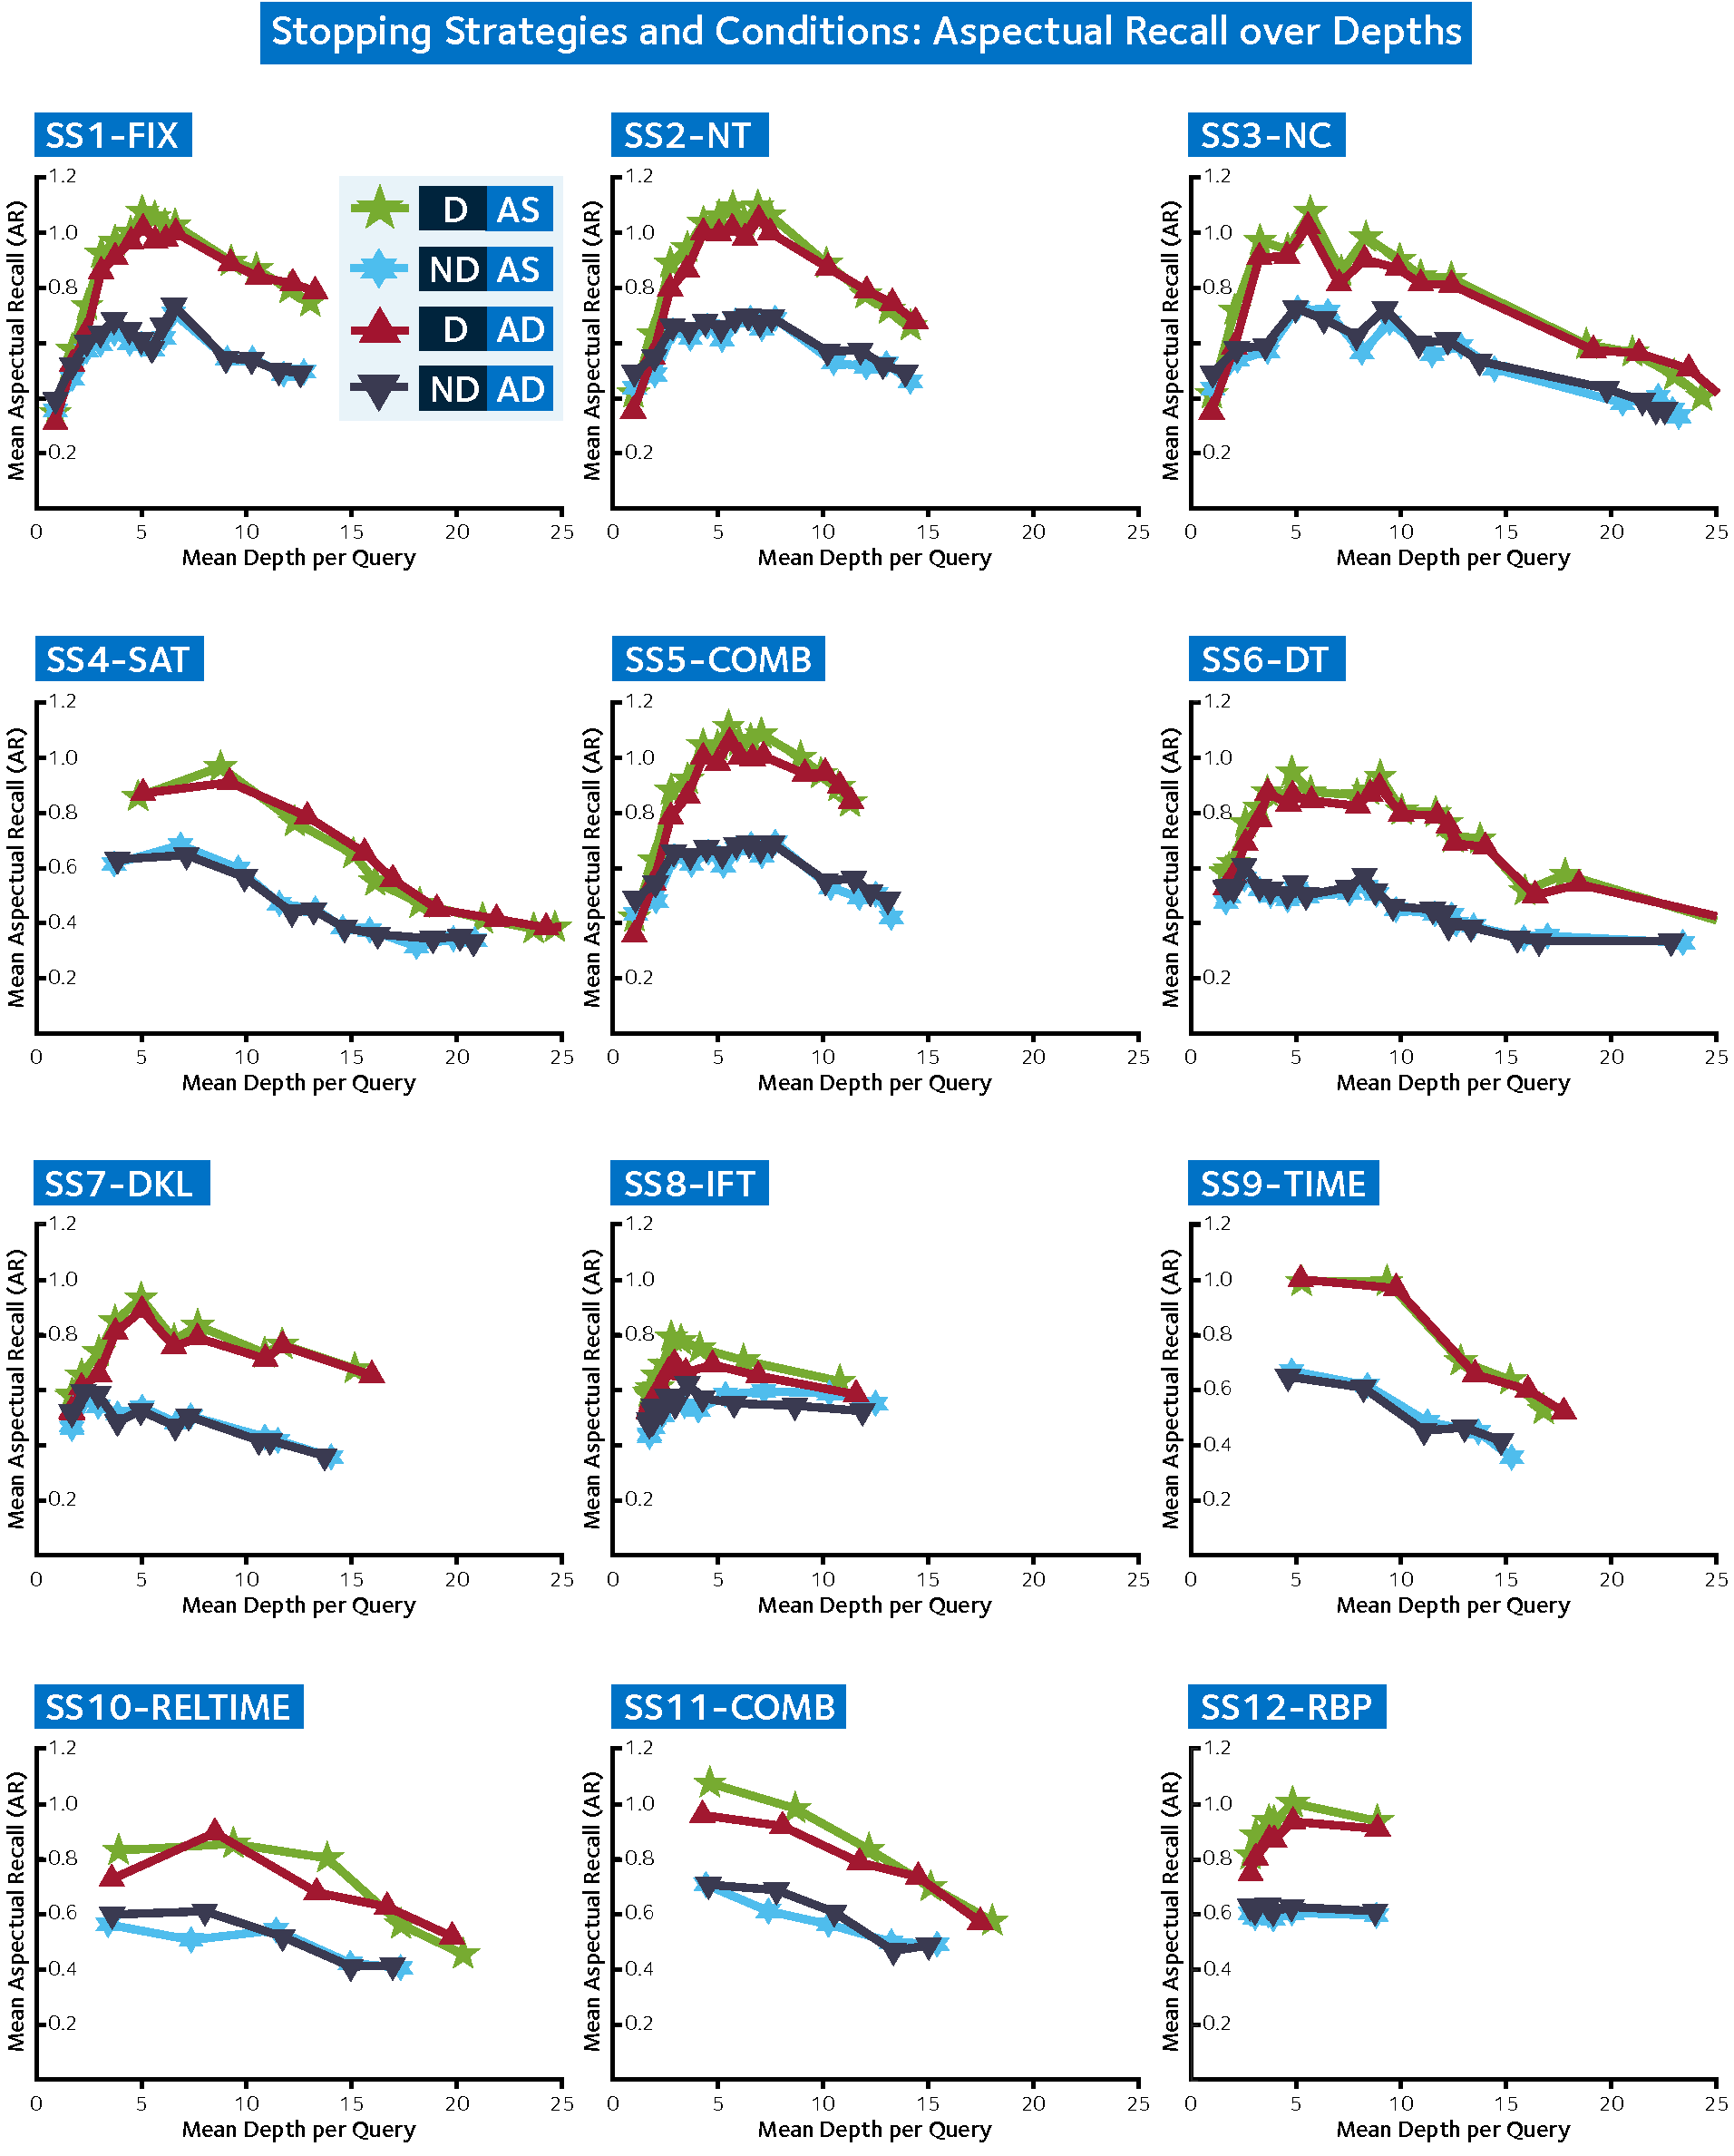
\includegraphics{figures/ch8-ar_plots.pdf}}
    \caption[Aspectual recall plots (diversification)]{Aspectual recall (documents containing at least one new entity) over the mean depth per query for each result summary level stopping strategy, in turn over each of the four experimental conditions. Note the profound gaps between the two tasks using diversified system \blueboxbold{D} and non-diversified system \blueboxbold{ND}. The depth per query reported on each \emph{x} axis is cut at 25.}
    \label{fig:ch8_sim_ar_plots}
\end{figure}

Indeed, a higher mean level of~\gls{acr:cg} correlates strongly with a higher mean level of AR -- an intuitive yet unsurprising result. In order to attain gain, one must save documents, and by saving documents, a simulated searcher will also identify documents with unseen aspects. Trends illustrate that like Figure~\ref{fig:ch8_sim_perf_plots}, plots build up to a peak before slowly diminishing as the mean depth per query increases. We also observe that a much higher level of AR is attained by tasks using system \blueboxbold{D}. For example, \blueboxbold{SS5-COMB} attains a maximum AR of $1.04$ and a mean depth per query of $4.21$, and $0.69$ at a mean depth per query of $7.65$ under conditions \dualbluebox{D}{AS} and \dualbluebox{ND}{AS} respectively. These results provide further proof that the diversification algorithm employed was successfully able to return a modified ranking with a more diverse set of results.

Turning our attention to the remaining stopping strategies, we first consider our fixed-depth baseline \blueboxbold{SS1-FIX}, in addition to frustration-based strategies \blueboxbold{SS2-NT}, \blueboxbold{SS3-NC}. All three perform remarkably well, with \blueboxbold{SS1-FIX} indeed offering best performance for condition \dualbluebox{ND}{AD}. Under condition \dualbluebox{D}{AS} for example, the three strategies offer a maximum~\gls{acr:cg} of $2.19$, $2.18$ and $2.20$ for the first three strategies in order, respectively. This is compared to the maximum reached by \blueboxbold{SS5-COMB} of $2.21$. In addition, the strategies all offer these levels of~\gls{acr:cg} at similar mean depths per query, suggesting that such approaches are just as robust as the combination strategy. This perhaps is an unsurprising finding, as \blueboxbold{SS5-COMB} utilises \blueboxbold{SS2-NT} as its frustration-based component.

Considering our time-based stopping strategies \blueboxbold{SS9-TIME} and \blueboxbold{SS10-RELTIME}, we find that \blueboxbold{SS9-TIME} consistently delivers the best performance across the four experimental conditions. This result is perhaps somewhat surprising, and mirrors findings from Section~\ref{sec:snippets:simulations:results:perf} -- an adaptive approach such as \blueboxbold{SS10-RELTIME} would intuitively make more sense, as the searcher would be able to adapt his or her stopping behaviour based upon the amount of relevant content found, rather than simply stopping after $30$ or $60$ seconds have elapsed from the point at which they begin their examination of results.

Considering our measure-based strategy \blueboxbold{SS12-RBP}, performance offered across the four conditions is somewhat poorer than the other strategies. However, no significant differences in performance were observed with this stopping strategy. Once notable aspects regarding the results for this strategy is the relatively shallow mean depth per query that simulated searchers traversed to on average. For tasks employing system \blueboxbold{ND}, results are particularly invariant -- no obvious peak in performance is observed.

The difference threshold stopping strategies \blueboxbold{SS6-DT} and \blueboxbold{SS7-DKL} yielded similar performance when compared to \blueboxbold{SS12-RBP}. However, simulated searchers subscribing to the difference strategies both traversed result lists to greater depths on average. Performance from these strategies perhaps was hindered by the querying strategy that we employed, and demonstrates that they are not particularly robust to detecting poor quality result lists.

The~\gls{acr:ift}-based stopping strategy \blueboxbold{SS8-IFT} however consistently performed the worst over all four experimental conditions. As can be observed from Figure~\ref{fig:ch8_sim_perf_plots}, we can see that the aforementioned gap between the two systems was not present, with all four tasks bunched very closely together across the range of mean depths per query. Indeed, performance across tasks utilising system \blueboxbold{D} was significantly different from the best performing strategy, \blueboxbold{SS5-COMB}.~\gls{acr:cg} reached $1.68$ and $1.46$ for tasks \dualbluebox{D}{AS} and \dualbluebox{D}{AD} respectively at relatively low mean depths per query. This suggests that the strategy was stopping too early, which is indicative to an incorrectly set rate of gain. This, and other aspects from our findings, are discussed in Chapter~\ref{chap:conclusions}.

\subsubsection{Real-World Comparisons}\label{sec:diversity:simulated:results:comparisons}
We now move our attention away from an examination of our simulated \emph{what-if} performance runs. We focus instead upon an examination of our real-world searcher comparison runs. These simulations provide a means for us to address \darkblueboxbold{HL-RQ3b}, under the context of varying task types and goals. As a reminder, we \emph{replayed} all of the queries issued by the real-world searchers, allowing for us to make a direct comparison between simulated and real-world click depths, indicative of a searcher's stopping behaviours.

Figure~\ref{fig:ch8_sim_comparison_plots} provides a total of twelve plots, one per result summary level stopping strategy. Within the plots are four lines, one representing the approximations offered by each of the four conditions for a given stopping strategy. Along the $x$ axes is the mean depth per query, with the $y$ axes this time denoting the MSE of the real-world vs. simulated click depths for the given stopping strategy and experimental condition combination.\footnote{Refer to Section~\ref{sec:method:simulation:runs:comparison} on page~\pageref{sec:method:simulation:runs:comparison} for further information on how we computed the \emph{Mean Squared Error (MSE).}} Each point on the plotted lines represents a stopping threshold parameter configuration. The closer the MSE tends to zero, the better the approximation to actual searcher stopping behaviours. For reference, we also include four dashed vertical lines on each of the plots in Figure~\ref{fig:ch8_sim_comparison_plots}. These lines represent the mean click depths that reached by the real-world searchers, over a given experimental condition. The closer the lowest MSE on a given simulation reaches the corresponding real-world mean click depth, the better the approximation. For example, the last point for condition \dualbluebox{D}{AS} under stopping strategy \blueboxbold{SS1-FIX} comes very close to the real-world click depth mean of $12.85$, compared to the simulation result of $13.25$. However, under \blueboxbold{SS7-DKL}, the same condition reaches comparatively shallower depths compared to the corresponding real-world mean, resulting in a higher MSE.

\begin{figure}[p!]
    \centering
    \resizebox{1\hsize}{!}{
    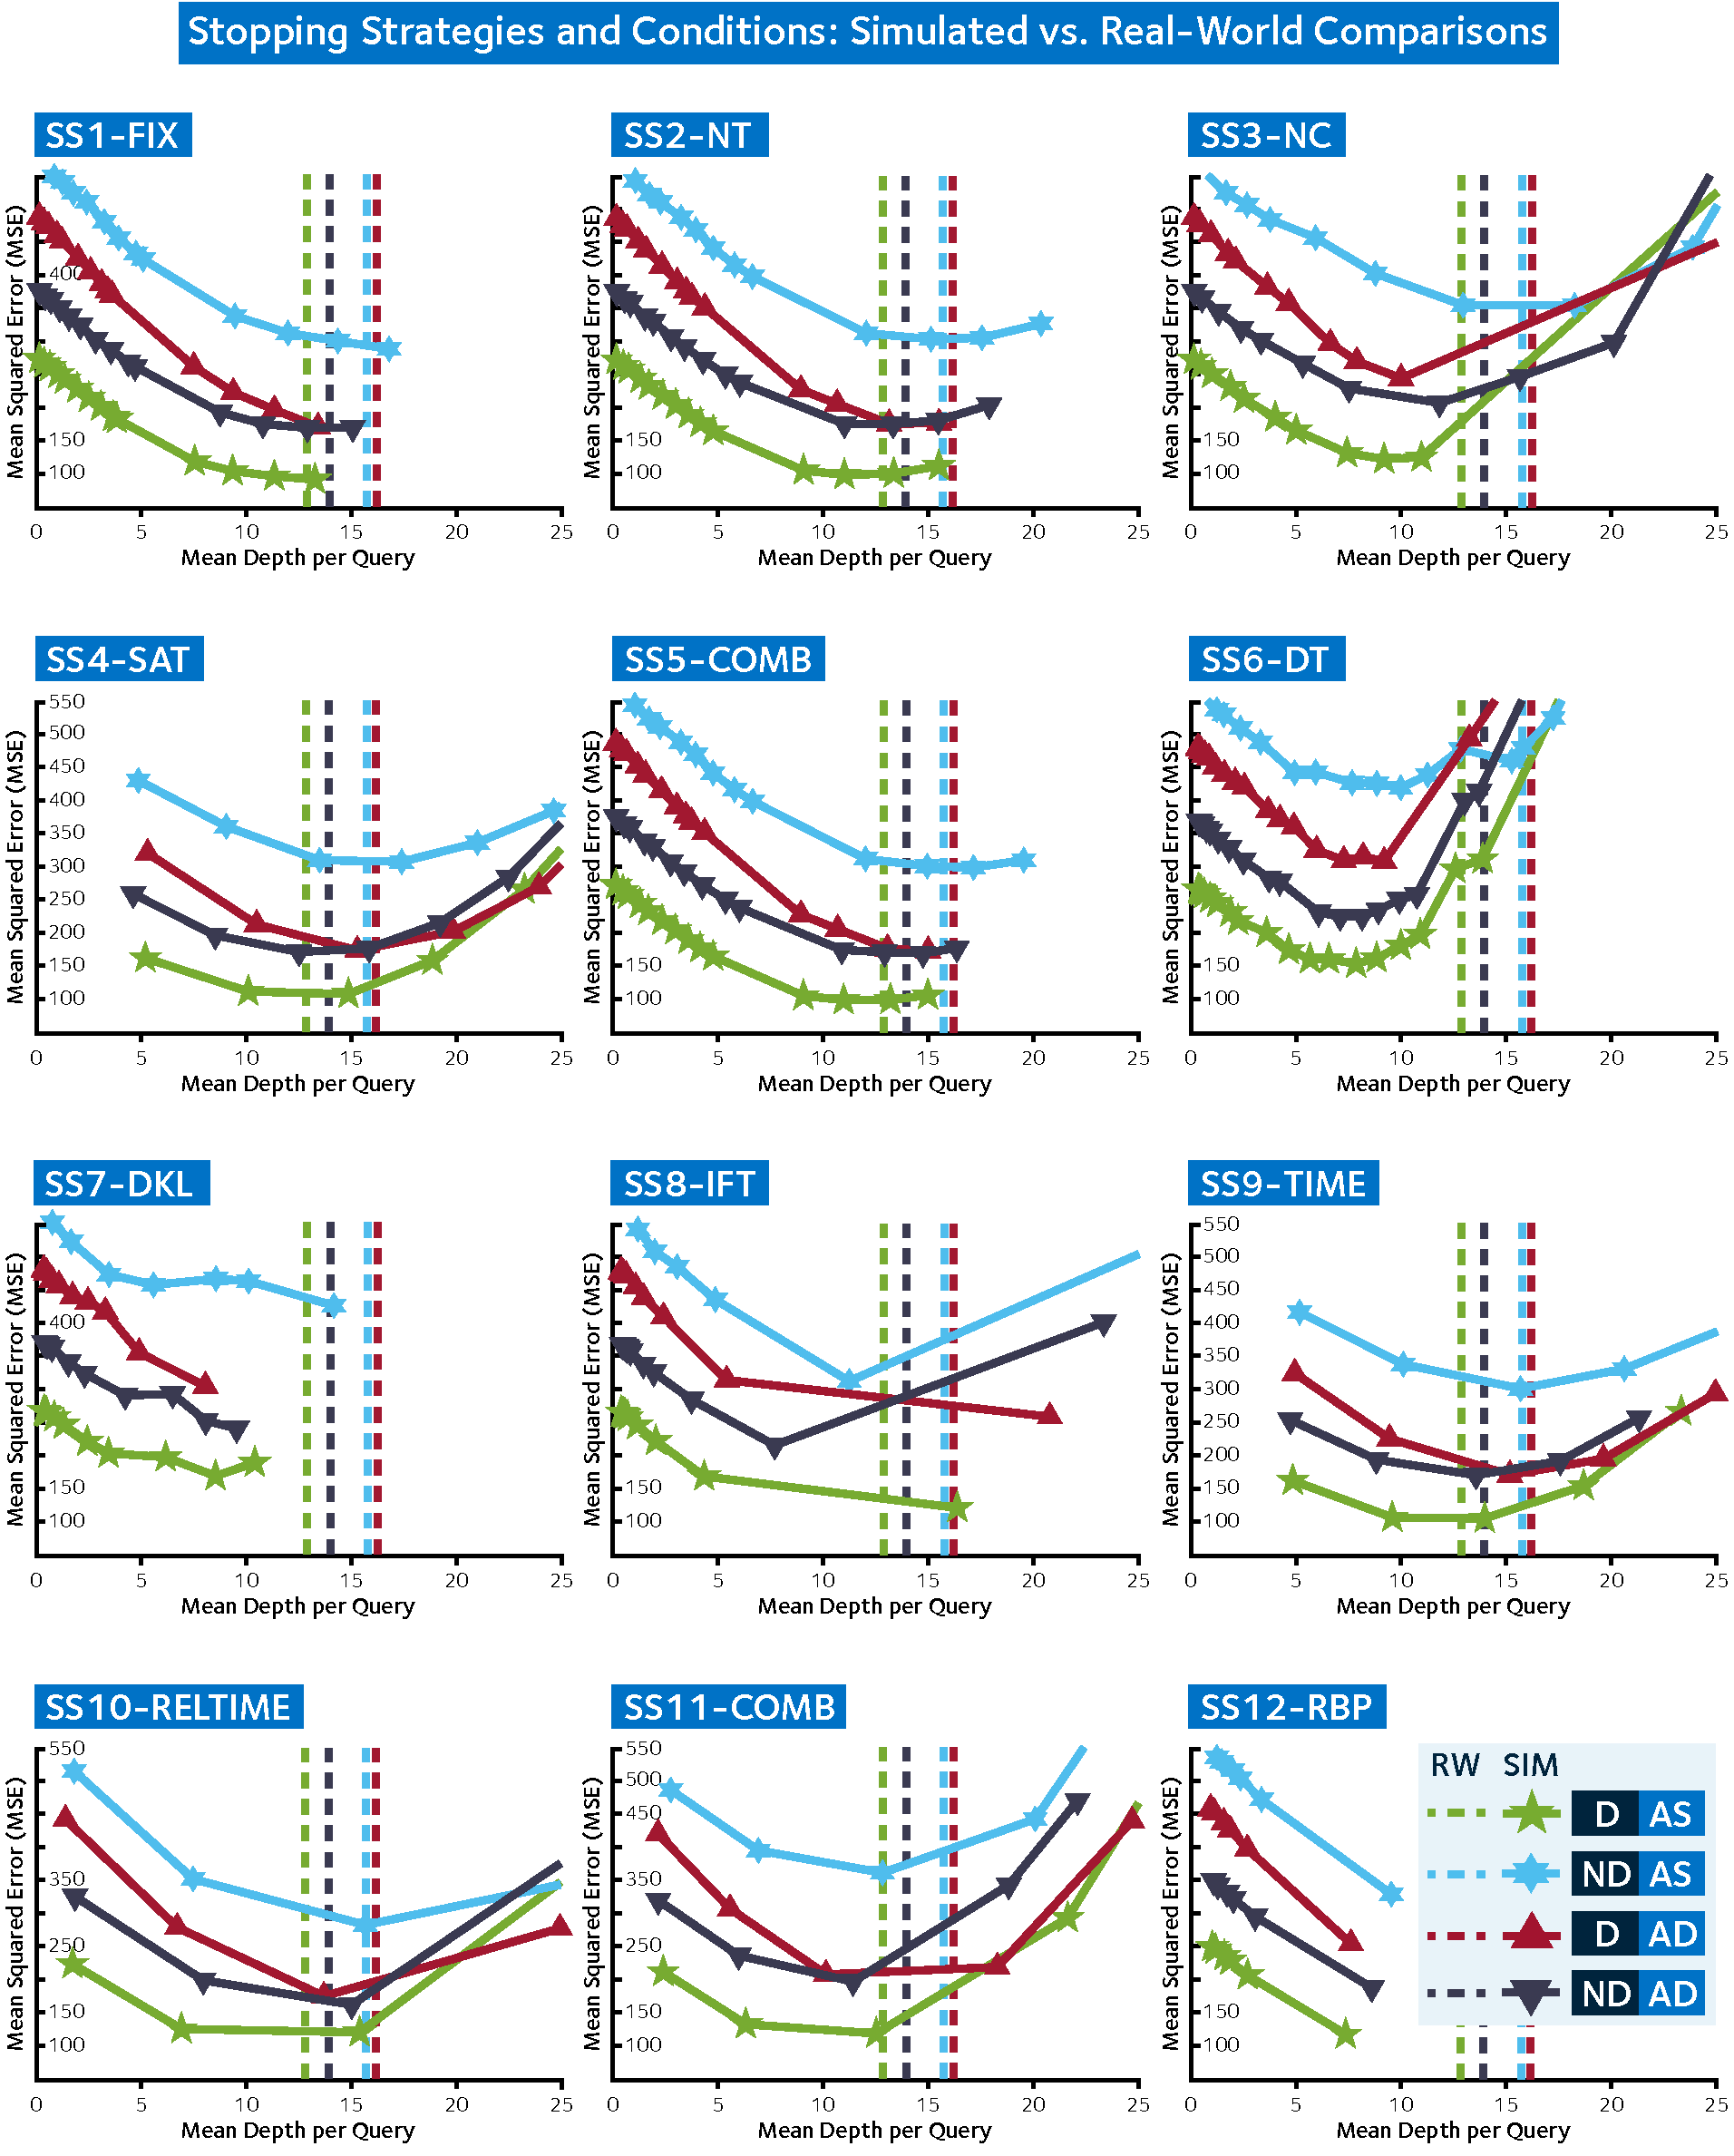
\includegraphics{figures/ch8-comparison_plots.pdf}}
    \caption[Comparison plots (diversification)]{Plots reporting the comparison runs, reporting the MSE vs. the mean depth per query. Runs over each of the four experimental conditions are shown. Also included in the plots are a series of dashed lines denoting the mean depth per query reached by the real-world subjects of the user study.}
    \label{fig:ch8_sim_comparison_plots}
\end{figure}

From the plots in Figure~\ref{fig:ch8_sim_comparison_plots}, we can observe a number of notable trends. One of the first points of note is the consistent ordering of the different conditions across the twelve stopping strategies. Remembering that the \emph{lower} the MSE value the better, we see that \dualbluebox{D}{AS} consistently offers the best approximations, especially at lower mean depths per query. This is then followed by \dualbluebox{ND}{AD}, \dualbluebox{D}{AD} and finally \dualbluebox{ND}{AS}. Note that unlike the results of the performance \emph{(what-if)} simulations reported in Section~\ref{sec:diversity:simulated:results:perf}, there is a distinct lack of separation between the two experimental systems trialled, namely \blueboxbold{ND} and \blueboxbold{D}. We also see smooth curves from stopping strategies such as \blueboxbold{SS1-FIX}, \blueboxbold{SS2-NT} and \blueboxbold{SS5-COMB} that offered good levels of performance from simulations reported in Section~\ref{sec:diversity:simulated:results:perf}. Conversely, strategies that performed poorly also appear to have more variable and inconsistent plots, such as those shown by \blueboxbold{SS7-DKL}, \blueboxbold{SS8-IFT}. These plots demonstrate that the approximations offered by the stopping strategies are inconsistent across mean depths per query, leading to the poorer approximations.

Given these trends, what stopping strategies offer the \emph{lowest,} and therefore best approximations of actual searcher stopping behaviours? Table~\ref{tbl:ch8_sim_comp} presents for each stopping strategy (over each condition) the point on the corresponding plots in Figure~\ref{fig:ch8_sim_comparison_plots} where the lowest MSE value is attained \genericblack{(MSE)}, and the stopping threshold value(s) \genericblack{(x\textsubscript{n})} that were used to attain it. Note that for condition \dualbluebox{D}{AS}, generally lower MSE values are attained than the other conditions. The table also \darkbluebox{highlights} the stopping strategy that yielded the lowest MSE for each condition. Interestingly, the baseline, fixed-depth stopping strategy \blueboxbold{SS1-FIX} offered the best approximations for conditions \dualbluebox{D}{AS} and \dualbluebox{D}{AD}, both of which were using diversified system \blueboxbold{D}. In comparison, conditions \dualbluebox{ND}{AS} and \dualbluebox{ND}{AD} were both found to demonstrate \blueboxbold{SS10-RELTIME} as yielding the best approximations to actual searcher stopping behaviour. These interesting results demonstrate a consistent finding, and we comment on the reasoning behind this finding in Chapter~\ref{chap:conclusions}. Indeed, consistency is also observed across the stopping parameter thresholds that yield the lowest MSE -- for \blueboxbold{SS1-FIX}, a depth of $24$ is cited as yielding the best approximations, with the best approximations under \blueboxbold{SS10-RELTIME} yielded $30$ seconds after the last relevant document had been saved.

\begin{table}[p!]
    \caption[Lowest MSE values for diversification comparisons runs]{Results from the simulated comparison runs, showing the \emph{lowest} MSE value reached over each result summary level stopping strategy trialled. \emph{x\textsubscript{n}} denotes the parameter threshold(s) that the lowest MSE was reached with. Results are presented across the four experimental conditions. For each condition, the stopping strategy that attained the lowest MSE is \darkbluebox{highlighted}. For the combination stopping strategies, two parameters are presented, with \emph{x\textsubscript{2},x\textsubscript{4}} presented for \blueboxbold{SS5-COMB} and \emph{x\textsubscript{10},x\textsubscript{4}} presented for \blueboxbold{SS11-COMB}. Significance testing yielded no significant differences between the stopping strategies at $\alpha$\emph{=0.05.}}
    \label{tbl:ch8_sim_comp}
    \renewcommand{\arraystretch}{1.8}
    \begin{center}
        \begin{tabulary}{\textwidth}{L{0.00cm}@{\CS}L{1.15cm}@{\CS}D{0.85cm}@{\CS}D{0.85cm}@{\CSONEHALF}D{0.85cm}@{\CS}D{0.85cm}@{\CSONEHALF}D{0.85cm}@{\CS}D{0.85cm}@{\CSONEHALF}D{0.85cm}@{\CS}D{0.85cm}@{\CSONEHALF}D{0.85cm}@{\CS}D{0.85cm}}
            
            & & \multicolumn{2}{@{\hskip 0pt}c@{\CSONEHALF}}{\dbluecell\small\textbf{D-AS}} & \multicolumn{2}{@{\hskip 0pt}c@{\CSONEHALF}}{\dbluecell\small\textbf{ND-AS}} & \multicolumn{2}{@{\hskip 0pt}c@{\CSONEHALF}}{\dbluecell\small\textbf{D-AD}} & \multicolumn{2}{@{\hskip 0pt}c@{\CSONEHALF}}{\dbluecell\small\textbf{ND-AD}} & \multicolumn{2}{@{\hskip 0pt}c@{\hskip 6pt}}{\dbluecell\small\textbf{Average}}\\
            
            \RS & & \lbluecell\small\textbf{x\textsubscript{n}} & \lbluecell\small\textbf{MSE} & \lbluecell\small\textbf{x\textsubscript{n}} & \lbluecell\small\textbf{MSE} & \lbluecell\small\textbf{x\textsubscript{n}} & \lbluecell\small\textbf{MSE} & \lbluecell\small\textbf{x\textsubscript{n}} & \lbluecell\small\textbf{MSE} & \lbluecell\small\textbf{x\textsubscript{n}} & \lbluecell\small\textbf{MSE} \\
            
            \RS \multirow{1}{*}{\hspace*{-2mm}\rotatebox{90}{\hspace*{-1mm}\small\textbf{FIX}}} & \lbluecell\small\textbf{SS1} & \dbluecell \small \hspace*{-1mm} 24 & \dbluecell \small \hspace*{-1.5mm} 90.27  & \cell \small \hspace*{-1mm} 24 & \cell \small \hspace*{-2.5mm} 287.50  & \dbluecell \small \hspace*{-1mm} 24 & \dbluecell \small \hspace*{-2.5mm} 169.62  & \cell \small \hspace*{-1mm} 21 & \cell \small \hspace*{-2.5mm} 168.39 & \dbluecell \small \hspace*{-1mm} 24 & \dbluecell \small \hspace*{-2.5mm} 179.03 \\
            
            \RS\RS\RS \multirow{2}{*}{\hspace*{-2mm}\rotatebox{90}{\hspace*{-3mm}\small\textbf{FRUS}}} & \lbluecell\small\textbf{SS2} & \cell \small \hspace*{-1mm} 18 & \cell \small \hspace*{-1.5mm} 98.49  & \cell \small \hspace*{-1mm} 18 & \cell \small \hspace*{-2.5mm} 303.84  & \cell \small \hspace*{-1mm} 21 & \cell \small \hspace*{-2.5mm} 175.76  & \cell \small \hspace*{-1mm} 18 & \cell \small \hspace*{-2.5mm} 175.39 & \cell \small \hspace*{-1mm} 21 & \cell \small \hspace*{-2.5mm} 190.83 \\
            
            \RS & \lbluecell\small\textbf{SS3} & \cell \small \hspace*{-1mm} 9 & \cell \small \hspace*{-2.5mm} 123.04  & \cell \small \hspace*{-1mm} 9 & \cell \small \hspace*{-2.5mm} 354.20  & \cell \small \hspace*{-1mm} 10 & \cell \small \hspace*{-2.5mm} 244.59  & \cell \small \hspace*{-1mm} 8 & \cell \small \hspace*{-2.5mm} 207.71 & \cell \small \hspace*{-1mm} 8 & \cell \small \hspace*{-2.5mm} 247.90 \\
            
            \RS\RS\RS \multirow{1}{*}{\hspace*{-2mm}\rotatebox{90}{\small\textbf{SAT}}} & \lbluecell\small\textbf{SS4} & \cell \small \hspace*{-1mm} 3 & \cell \small \hspace*{-2.5mm} 107.38  & \cell \small \hspace*{-1mm} 4 & \cell \small \hspace*{-2.5mm} 307.00  & \cell \small \hspace*{-1mm} 3 & \cell \small \hspace*{-2.5mm} 173.16  & \cell \small \hspace*{-1mm} 3 & \cell \small \hspace*{-2.5mm} 170.68 & \cell \small \hspace*{-1mm} 3 & \cell \small \hspace*{-2.5mm} 190.14 \\
            
            \RS\RS\RS \multirow{1}{*}{\hspace*{-2mm}\rotatebox{90}{\small\textbf{COM}}} & \lbluecell\small\textbf{SS5} & \cell \small \hspace*{-1mm} 24,3 & \cell \small \hspace*{-1.5mm} 93.79  & \cell \small \hspace*{-1mm} 21,5 & \cell \small \hspace*{-2.5mm} 288.30  & \cell \small \hspace*{-1mm} 24,6 & \cell \small \hspace*{-2.5mm} 173.23  & \cell \small \hspace*{-1mm} 21,5 & \cell \small \hspace*{-2.5mm} 162.81 & \cell \small \hspace*{-1mm} 21,5 & \cell \small \hspace*{-2.5mm} 181.12 \\
            
            \RS\RS\RS \multirow{2}{*}{\hspace*{-2mm}\rotatebox{90}{\small\textbf{DIFF}}} & \lbluecell\small\textbf{SS6} & \cell \small \hspace*{-1mm} 0.70 & \cell \small \hspace*{-2.5mm} 154.08  & \cell \small \hspace*{-1mm} 0.70 & \cell \small \hspace*{-2.5mm} 418.69  & \cell \small \hspace*{-1mm} 0.85 & \cell \small \hspace*{-2.5mm} 307.94  & \cell \small \hspace*{-1mm} 0.65 & \cell \small \hspace*{-2.5mm} 224.88 & \cell \small \hspace*{-1mm} 0.70 & \cell \small \hspace*{-2.5mm} 280.81 \\
            
            \RS & \lbluecell\small\textbf{SS7} & \cell \small \hspace*{-1mm} 3.5 & \cell \small \hspace*{-2.5mm} 168.04  & \cell \small \hspace*{-1mm} 3.0 & \cell \small \hspace*{-2.5mm} 424.14  & \cell \small \hspace*{-1mm} 3.0 & \cell \small \hspace*{-2.5mm} 303.07  & \cell \small \hspace*{-1mm} 3.0 & \cell \small \hspace*{-2.5mm} 239.57 & \cell \small \hspace*{-1mm} 3.0 & \cell \small \hspace*{-2.5mm} 288.72 \\
            
            \RS\RS\RS \multirow{1}{*}{\hspace*{-2mm}\rotatebox{90}{\small\textbf{IFT}}} & \lbluecell\small\textbf{SS8} & \cell \small \hspace*{-1mm} 0.002 & \cell \small \hspace*{-2.5mm} 120.96  & \cell \small \hspace*{-1mm} 0.004 & \cell \small \hspace*{-2.5mm} 312.39  & \cell \small \hspace*{-1mm} 0.002 & \cell \small \hspace*{-2.5mm} 258.71  & \cell \small \hspace*{-1mm} 0.004 & \cell \small \hspace*{-2.5mm} 215.60 & \cell \small \hspace*{-1mm} 0.004 & \cell \small \hspace*{-2.5mm} 252.71 \\
            
            \RS\RS\RS \multirow{2}{*}{\hspace*{-2mm}\rotatebox{90}{\hspace*{-2mm}\small\textbf{TIME}}} & \lbluecell\small\textbf{SS9} & \cell \small \hspace*{-1mm} 90 & \cell \small \hspace*{-2.5mm} 105.68  & \cell \small \hspace*{-1mm} 90 & \cell \small \hspace*{-2.5mm} 300.81  & \cell \small \hspace*{-1mm} 90 & \cell \small \hspace*{-2.5mm} 171.19  & \cell \small \hspace*{-1mm} 90 & \cell \small \hspace*{-2.5mm} 170.88 & \cell \small \hspace*{-1mm} 90 & \cell \small \hspace*{-2.5mm} 187.14 \\
            
            \RS & \lbluecell\small\textbf{SS10} & \cell \small \hspace*{-1mm} 30 & \cell \small \hspace*{-2.5mm} 120.43  & \dbluecell \small \hspace*{-1mm} 30 & \dbluecell \small \hspace*{-2.5mm} 282.86  & \cell \small \hspace*{-1mm} 30 & \cell \small \hspace*{-2.5mm} 174.96  & \dbluecell \small \hspace*{-1mm} 30 & \dbluecell \small \hspace*{-2.5mm} 162.19 & \cell \small \hspace*{-1mm} 30 & \cell \small \hspace*{-2.5mm} 185.11 \\
            
            \RS\RS\RS \multirow{1}{*}{\hspace*{-2mm}\rotatebox{90}{\small\textbf{COM}}} & \lbluecell\small\textbf{SS11} & \cell \small \hspace*{-1mm} 30,5 & \cell \small \hspace*{-2.5mm} 117.50  & \cell \small \hspace*{-1mm} 30,7 & \cell \small \hspace*{-2.5mm} 360.06  & \cell \small \hspace*{-1mm} 30,5 & \cell \small \hspace*{-2.5mm} 206.59  & \cell \small \hspace*{-1mm} 30,5 & \cell \small \hspace*{-2.5mm} 187.68 & \cell \small \hspace*{-1mm} 30,5 & \cell \small \hspace*{-2.5mm} 218.25 \\
            
            \RS\RS\RS \multirow{1}{*}{\hspace*{-2mm}\rotatebox{90}{\small\textbf{RBP}}} & \lbluecell\small\textbf{SS12} & \cell \small \hspace*{-1mm} 0.99 & \cell \small \hspace*{-2.5mm} 118.09  & \cell \small \hspace*{-1mm} 0.99 & \cell \small \hspace*{-2.5mm} 330.16  & \cell \small \hspace*{-1mm} 0.99 & \cell \small \hspace*{-2.5mm} 255.20  & \cell \small \hspace*{-1mm} 0.99 & \cell \small \hspace*{-2.5mm} 188.53 & \cell \small \hspace*{-1mm} 0.99 & \cell \small \hspace*{-2.5mm} 222.99 \\
            
        \end{tabulary}
        \end{center}
    \end{table}

Given the fact that we observed consistent results across the systems trialled, we also decided to examine whether a particular stopping strategy emerged as providing good approximations over all four experimental conditions averaged together. Results from this analysis are shown in the \genericblack{Average} grouping in Table~\ref{tbl:ch8_sim_comp}. Statistical tests comparing the best approximating stopping strategy (again \dualbluebox{SS1-FIX}{@24}) against the remaining eleven stopping strategies yielded no statistically significant differences. Indeed, this was true across all four experimental conditions when considered in isolation. This result highlights that all stopping strategies offered similar approximations. As no statistical differences emerged when considering the average of the four experimental conditions, we do not explore this avenue any further.

Moving back to our per-condition examination, Table~\ref{tbl:ch8_sim_comp_cgdq} repots additional information relating to the best approximation offered by each stopping strategy. We report for each stopping strategy the: mean depth per query \genericblack{(DQ)}; the mean number of saved and~\gls{acr:trec} relevant documents \genericblack{\#S}; and the mean \genericblack{AR}, denoting the number of saved,~\gls{acr:trec} relevant documents containing at least one new aspect. The values reported in the table were attained at the stopping threshold parameter(s) that yielded the lowest MSE, as reported in Table~\ref{tbl:ch8_sim_comp}. Also included in Table~\ref{tbl:ch8_sim_comp_cgdq} are the mean values for each measure that were attained by real-world subjects of the user study (represented as the \genericblack{RW}) column, included for easy comparison. We once again also \darkbluebox{highlight} the stopping strategy for each condition that yielded the lowest MSE.

Results observed from Table~\ref{tbl:ch8_sim_comp_cgdq} are largely as expected: stopping strategies that yielded close approximations to actual mean searcher behaviours offered mean depths per query that were similar to that of the real-world mean for the given condition. In contrast, we find that stopping strategies offering approximations with higher MSE values such as \blueboxbold{SS6-DT}, \blueboxbold{SS7-DKL} and \blueboxbold{SS8-IFT} do so at much lower or higher mean depths per query, although these differences are not significant. Results from Table~\ref{tbl:ch8_sim_comp_cgdq} also show that the simulated searchers on average saved fewer~\gls{acr:trec} relevant documents across all four experimental conditions, and, as a consequence, identified fewer~\gls{acr:trec} relevant documents with at least one new aspect. For example, across conditions \dualbluebox{D}{AS}, \dualbluebox{ND}{AS}, \dualbluebox{D}{AD} and \dualbluebox{ND}{AD}, real-world subjects saved $2.63$, $2.18$, $2.51$ and $2.22$~\gls{acr:trec} relevant documents on average. Across our fixed-depth baseline \blueboxbold{SS1-FIX}, simulated searchers saved $1.94$, $1.96$, $1.67$ and $1.66$~\gls{acr:trec} relevant documents on average. These comparatively low values may be an artefact of how we instantiated the simulations of interaction. We leave this discussion to Chapter~\ref{chap:conclusions}.

\begin{table}[p!]
    \caption[Additional comparison runs information (diversification)]{Additional results from the searcher comparisons runs, with this table reporting the mean depth per query. Also included are the mean number of saved,~\gls{acr:trec} relevant documents \emph{\#S (saved)} – and from that, the mean number of saved documents that contain one or more new aspects \emph{AR.} These are used for determining task completion for \darkblueboxbold{AD} and \darkblueboxbold{AS} tasks respectively. All these values are reported at the configuration yielding the lowest MSE (refer to Table~\ref{tbl:ch8_sim_comp}), indicating the best approximation to real-world stopping behaviours. We also include are the mean real-world \emph{(RW)} values over each condition for a direct comparison.}
    \label{tbl:ch8_sim_comp_cgdq}
    \renewcommand{\arraystretch}{1.8}
    
    \begin{center}
        \begin{tabulary}{\textwidth}{L{0.00cm}@{\CS}L{1cm}@{\CS}D{0.64cm}@{\CS}D{0.64cm}@{\CS}D{0.64cm}@{\CSONEHALF}D{0.64cm}@{\CS}D{0.64cm}@{\CS}D{0.64cm}@{\CSONEHALF}D{0.64cm}@{\CS}D{0.64cm}@{\CS}D{0.64cm}@{\CSONEHALF}D{0.64cm}@{\CS}D{0.64cm}@{\CS}D{0.64cm}@{\CS}}

            & & \multicolumn{3}{@{\hskip 0pt}c@{\CSONEHALF}}{\dbluecell\small\textbf{D-AS}} & \multicolumn{3}{@{\hskip 0pt}c@{\CSONEHALF}}{\dbluecell\small\textbf{ND-AS}} & \multicolumn{3}{@{\hskip 0pt}c@{\CSONEHALF}}{\dbluecell\small\textbf{D-AD}} & \multicolumn{3}{@{\hskip 0pt}c@{\CS}}{\dbluecell\small\textbf{ND-AD}}\\

            \RS & & \lbluecell\small\textbf{DQ} & \lbluecell\small\textbf{\#S} & \lbluecell\small\textbf{AR} & \lbluecell\small\textbf{DQ} & \lbluecell\small\textbf{\#S} & \lbluecell\small\textbf{AR} & \lbluecell\small\textbf{DQ} & \lbluecell\small\textbf{\#S} & \lbluecell\small\textbf{AR} & \lbluecell\small\textbf{DQ} & \lbluecell\small\textbf{\#S} & \lbluecell\small\textbf{AR} \\

            \RS & \dbluecell\small\textbf{RW} & \cell \small \hspace*{-2.5mm} 12.85 & \cell \small \hspace*{-1mm} 2.63 & \cell \hspace*{-1mm} \small 3.20 & \cell \small \hspace*{-2.5mm} 15.73 & \cell \small \hspace*{-1mm} 2.18 & \cell \hspace*{-1mm} \small 2.35 & \cell \small \hspace*{-2.5mm} 16.19 & \cell \small \hspace*{-1mm} 2.51 & \cell \hspace*{-1mm} \small 2.63 & \cell \small \hspace*{-2.5mm} 13.94 & \cell \small \hspace*{-1mm} 2.22 & \cell \hspace*{-1mm} \small 2.02 \\

            \RS\RS\RS \multirow{1}{*}{\hspace*{-2mm}\rotatebox{90}{\hspace*{-1mm}\small\textbf{FIX}}} & \lbluecell\small\textbf{SS1} & \dbluecell \small \hspace*{-2.5mm} 13.25 & \dbluecell \small \hspace*{-1mm} 1.94 & \dbluecell \hspace*{-1mm} \small 1.50 & \cell \small \hspace*{-2.5mm} 16.79 & \cell \small \hspace*{-1mm} 1.96 & \cell \hspace*{-1mm} \small 1.44 & \dbluecell \small \hspace*{-2.5mm} 13.40 & \dbluecell \small \hspace*{-1mm} 1.67 & \dbluecell \hspace*{-1mm} \small 1.42 & \cell \small \hspace*{-2.5mm} 12.89 & \cell \small \hspace*{-1mm} 1.66 & \cell \hspace*{-1mm} \small 1.26 \\

            \RS\RS\RS \multirow{2}{*}{\hspace*{-2mm}\rotatebox{90}{\hspace*{-3mm}\small\textbf{FRUS}}} & \lbluecell\small\textbf{SS2} & \cell \small \hspace*{-2.5mm} 11.01 & \cell \small \hspace*{-1mm} 2.04 & \cell \hspace*{-1mm} \small 1.58 & \cell \small \hspace*{-2.5mm} 15.15 & \cell \small \hspace*{-1mm} 1.91 & \cell \hspace*{-1mm} \small 1.43 & \cell \small \hspace*{-2.5mm} 13.15 & \cell \small \hspace*{-1mm} 1.75 & \cell \hspace*{-1mm} \small 1.48 & \cell \small \hspace*{-2.5mm} 13.34 & \cell \small \hspace*{-1mm} 1.77 & \cell \hspace*{-1mm} \small 1.33 \\

            \RS & \lbluecell\small\textbf{SS3} & \cell \small \hspace*{-1mm} 9.16 & \cell \small \hspace*{-1mm} 1.91 & \cell \hspace*{-1mm} \small 1.47 & \cell \small \hspace*{-2.5mm} 18.22 & \cell \small \hspace*{-1mm} 2.33 & \cell \hspace*{-1mm} \small 1.59 & \cell \small \hspace*{-1mm} 9.97 & \cell \small \hspace*{-1mm} 1.75 & \cell \hspace*{-1mm} \small 1.43 & \cell \small \hspace*{-2.5mm} 11.80 & \cell \small \hspace*{-1mm} 1.73 & \cell \hspace*{-1mm} \small 1.25 \\

            \RS\RS\RS \multirow{1}{*}{\hspace*{-2mm}\rotatebox{90}{\small\textbf{SAT}}} & \lbluecell\small\textbf{SS4} & \cell \small \hspace*{-2.5mm} 14.87 & \cell \small \hspace*{-1mm} 1.89 & \cell \hspace*{-1mm} \small 1.54 & \cell \small \hspace*{-2.5mm} 17.40 & \cell \small \hspace*{-1mm} 1.73 & \cell \hspace*{-1mm} \small 1.32 & \cell \small \hspace*{-2.5mm} 15.29 & \cell \small \hspace*{-1mm} 1.70 & \cell \hspace*{-1mm} \small 1.48 & \cell \small \hspace*{-2.5mm} 12.51 & \cell \small \hspace*{-1mm} 1.27 & \cell \hspace*{-1mm} \small 0.96 \\

            \RS\RS\RS \multirow{1}{*}{\hspace*{-2mm}\rotatebox{90}{\small\textbf{COM}}} & \lbluecell\small\textbf{SS5} & \cell \small \hspace*{-2.5mm} 11.62 & \cell \small \hspace*{-1mm} 1.81 & \cell \hspace*{-1mm} \small 1.48 & \cell \small \hspace*{-2.5mm} 15.43 & \cell \small \hspace*{-1mm} 1.86 & \cell \hspace*{-1mm} \small 1.43 & \cell \small \hspace*{-2.5mm} 14.98 & \cell \small \hspace*{-1mm} 1.80 & \cell \hspace*{-1mm} \small 1.49 & \cell \small \hspace*{-2.5mm} 14.16 & \cell \small \hspace*{-1mm} 1.75 & \cell \hspace*{-1mm} \small 1.32 \\

            \RS\RS\RS \multirow{2}{*}{\hspace*{-2mm}\rotatebox{90}{\small\textbf{DIFF}}} & \lbluecell\small\textbf{SS6} & \cell \small \hspace*{-1mm} 7.85 & \cell \small \hspace*{-1mm} 1.36 & \cell \hspace*{-1mm} \small 1.11 & \cell \small \hspace*{-1mm} 9.97 & \cell \small \hspace*{-1mm} 1.25 & \cell \hspace*{-1mm} \small 0.94 & \cell \small \hspace*{-1mm} 9.19 & \cell \small \hspace*{-1mm} 1.50 & \cell \hspace*{-1mm} \small 1.25 & \cell \small \hspace*{-1mm} 7.10 & \cell \small \hspace*{-1mm} 1.05 & \cell \hspace*{-1mm} \small 0.81 \\

            \RS & \lbluecell\small\textbf{SS7} & \cell \small \hspace*{-1mm} 8.50 & \cell \small \hspace*{-1mm} 1.35 & \cell \hspace*{-1mm} \small 1.12 & \cell \small \hspace*{-2.5mm} 14.12 & \cell \small \hspace*{-1mm} 1.40 & \cell \hspace*{-1mm} \small 1.05 & \cell \small \hspace*{-1mm} 8.02 & \cell \small \hspace*{-1mm} 1.29 & \cell \hspace*{-1mm} \small 1.14 & \cell \small \hspace*{-1mm} 9.50 & \cell \small \hspace*{-1mm} 1.30 & \cell \hspace*{-1mm} \small 0.99 \\

            \RS\RS\RS \multirow{1}{*}{\hspace*{-2mm}\rotatebox{90}{\small\textbf{IFT}}} & \lbluecell\small\textbf{SS8} & \cell \small \hspace*{-2.5mm} 16.35 & \cell \small \hspace*{-1mm} 1.16 & \cell \hspace*{-1mm} \small 0.83 & \cell \small \hspace*{-2.5mm} 11.21 & \cell \small \hspace*{-1mm} 1.04 & \cell \hspace*{-1mm} \small 0.74 & \cell \small \hspace*{-2.5mm} 20.76 & \cell \small \hspace*{-1mm} 1.16 & \cell \hspace*{-1mm} \small 0.86 & \cell \small \hspace*{-1mm} 7.66 & \cell \small \hspace*{-1mm} 0.95 & \cell \hspace*{-1mm} \small 0.71 \\

            \RS\RS\RS \multirow{2}{*}{\hspace*{-2mm}\rotatebox{90}{\hspace*{-2mm}\small\textbf{TIME}}} & \lbluecell\small\textbf{SS9} & \cell \small \hspace*{-2.5mm} 13.96 & \cell \small \hspace*{-1mm} 1.92 & \cell \hspace*{-1mm} \small 1.49 & \cell \small \hspace*{-2.5mm} 15.66 & \cell \small \hspace*{-1mm} 1.76 & \cell \hspace*{-1mm} \small 1.33 & \cell \small \hspace*{-2.5mm} 15.15 & \cell \small \hspace*{-1mm} 1.71 & \cell \hspace*{-1mm} \small 1.46 & \cell \small \hspace*{-2.5mm} 13.55 & \cell \small \hspace*{-1mm} 1.49 & \cell \hspace*{-1mm} \small 1.12 \\

            \RS & \lbluecell\small\textbf{SS10} & \cell \small \hspace*{-2.5mm} 15.42 & \cell \small \hspace*{-1mm} 2.07 & \cell \hspace*{-1mm} \small 1.63 & \dbluecell \small \hspace*{-2.5mm} 15.69 & \dbluecell \small \hspace*{-1mm} 1.68 & \dbluecell \hspace*{-1mm} \small 1.25 & \cell \small \hspace*{-2.5mm} 13.72 & \cell \small \hspace*{-1mm} 1.83 & \cell \hspace*{-1mm} \small 1.55 & \dbluecell \small \hspace*{-2.5mm} 15.05 & \dbluecell \small \hspace*{-1mm} 1.50 & \dbluecell \hspace*{-1mm} \small 1.13 \\

            \RS\RS\RS \multirow{1}{*}{\hspace*{-2mm}\rotatebox{90}{\small\textbf{COM}}} & \lbluecell\small\textbf{SS11} & \cell \small \hspace*{-2.5mm} 12.54 & \cell \small \hspace*{-1mm} 1.75 & \cell \hspace*{-1mm} \small 1.44 & \cell \small \hspace*{-2.5mm} 12.81 & \cell \small \hspace*{-1mm} 1.48 & \cell \hspace*{-1mm} \small 1.14 & \cell \small \hspace*{-2.5mm} 10.14 & \cell \small \hspace*{-1mm} 1.58 & \cell \hspace*{-1mm} \small 1.37 & \cell \small \hspace*{-2.5mm} 11.71 & \cell \small \hspace*{-1mm} 1.35 & \cell \hspace*{-1mm} \small 1.03 \\

            \RS\RS\RS \multirow{1}{*}{\hspace*{-2mm}\rotatebox{90}{\small\textbf{RBP}}} & \lbluecell\small\textbf{SS12} & \cell \small \hspace*{-1mm} 7.36 & \cell \small \hspace*{-1mm} 1.54 & \cell \hspace*{-1mm} \small 1.30 & \cell \small \hspace*{-1mm} 9.54 & \cell \small \hspace*{-1mm} 1.29 & \cell \hspace*{-1mm} \small 1.00 & \cell \small \hspace*{-1mm} 7.61 & \cell \small \hspace*{-1mm} 1.39 & \cell \hspace*{-1mm} \small 1.25 & \cell \small \hspace*{-1mm} 8.61 & \cell \small \hspace*{-1mm} 1.19 & \cell \hspace*{-1mm} \small 0.92 \\

        \end{tabulary}
        \end{center}
    \end{table}

With the comparatively low numbers of~\gls{acr:trec} relevant documents saved, this also corresponds to a relatively low level of~\gls{acr:cg} when compared to the real-world means across conditions. Figure~\ref{fig:ch7_sim_comparison_rankings} reports the mean levels of~\gls{acr:cg} that were attained for each of the stopping strategies, along with the mean real-world~\gls{acr:cg} values for each experimental interface. These values were again computed from the stopping threshold parameter(s) that yielded the lowest MSE values, as reported in Table~\ref{tbl:ch8_sim_comp}. Bar charts provide a visual representation of~\gls{acr:cg} attained by each stopping strategy for each experimental condition, with the ranked values provided to the right of each chart. With real-world~\gls{acr:cg} values of $4.09$, $3.35$, $4.12$ and $3.49$ attained for conditions \dualbluebox{D}{AS}, \dualbluebox{ND}{AS}, \dualbluebox{D}{AD} and \dualbluebox{ND}{AD}, we can see that in all but condition \dualbluebox{ND}{AS}, the real-world searchers on average outperform all twelve stopping strategies. For condition \dualbluebox{ND}{AS}, \blueboxbold{SS3-NC} yielded a~\gls{acr:cg} value of $3.55$.

\begin{figure}[p!]
    \centering
    \resizebox{1\hsize}{!}{
    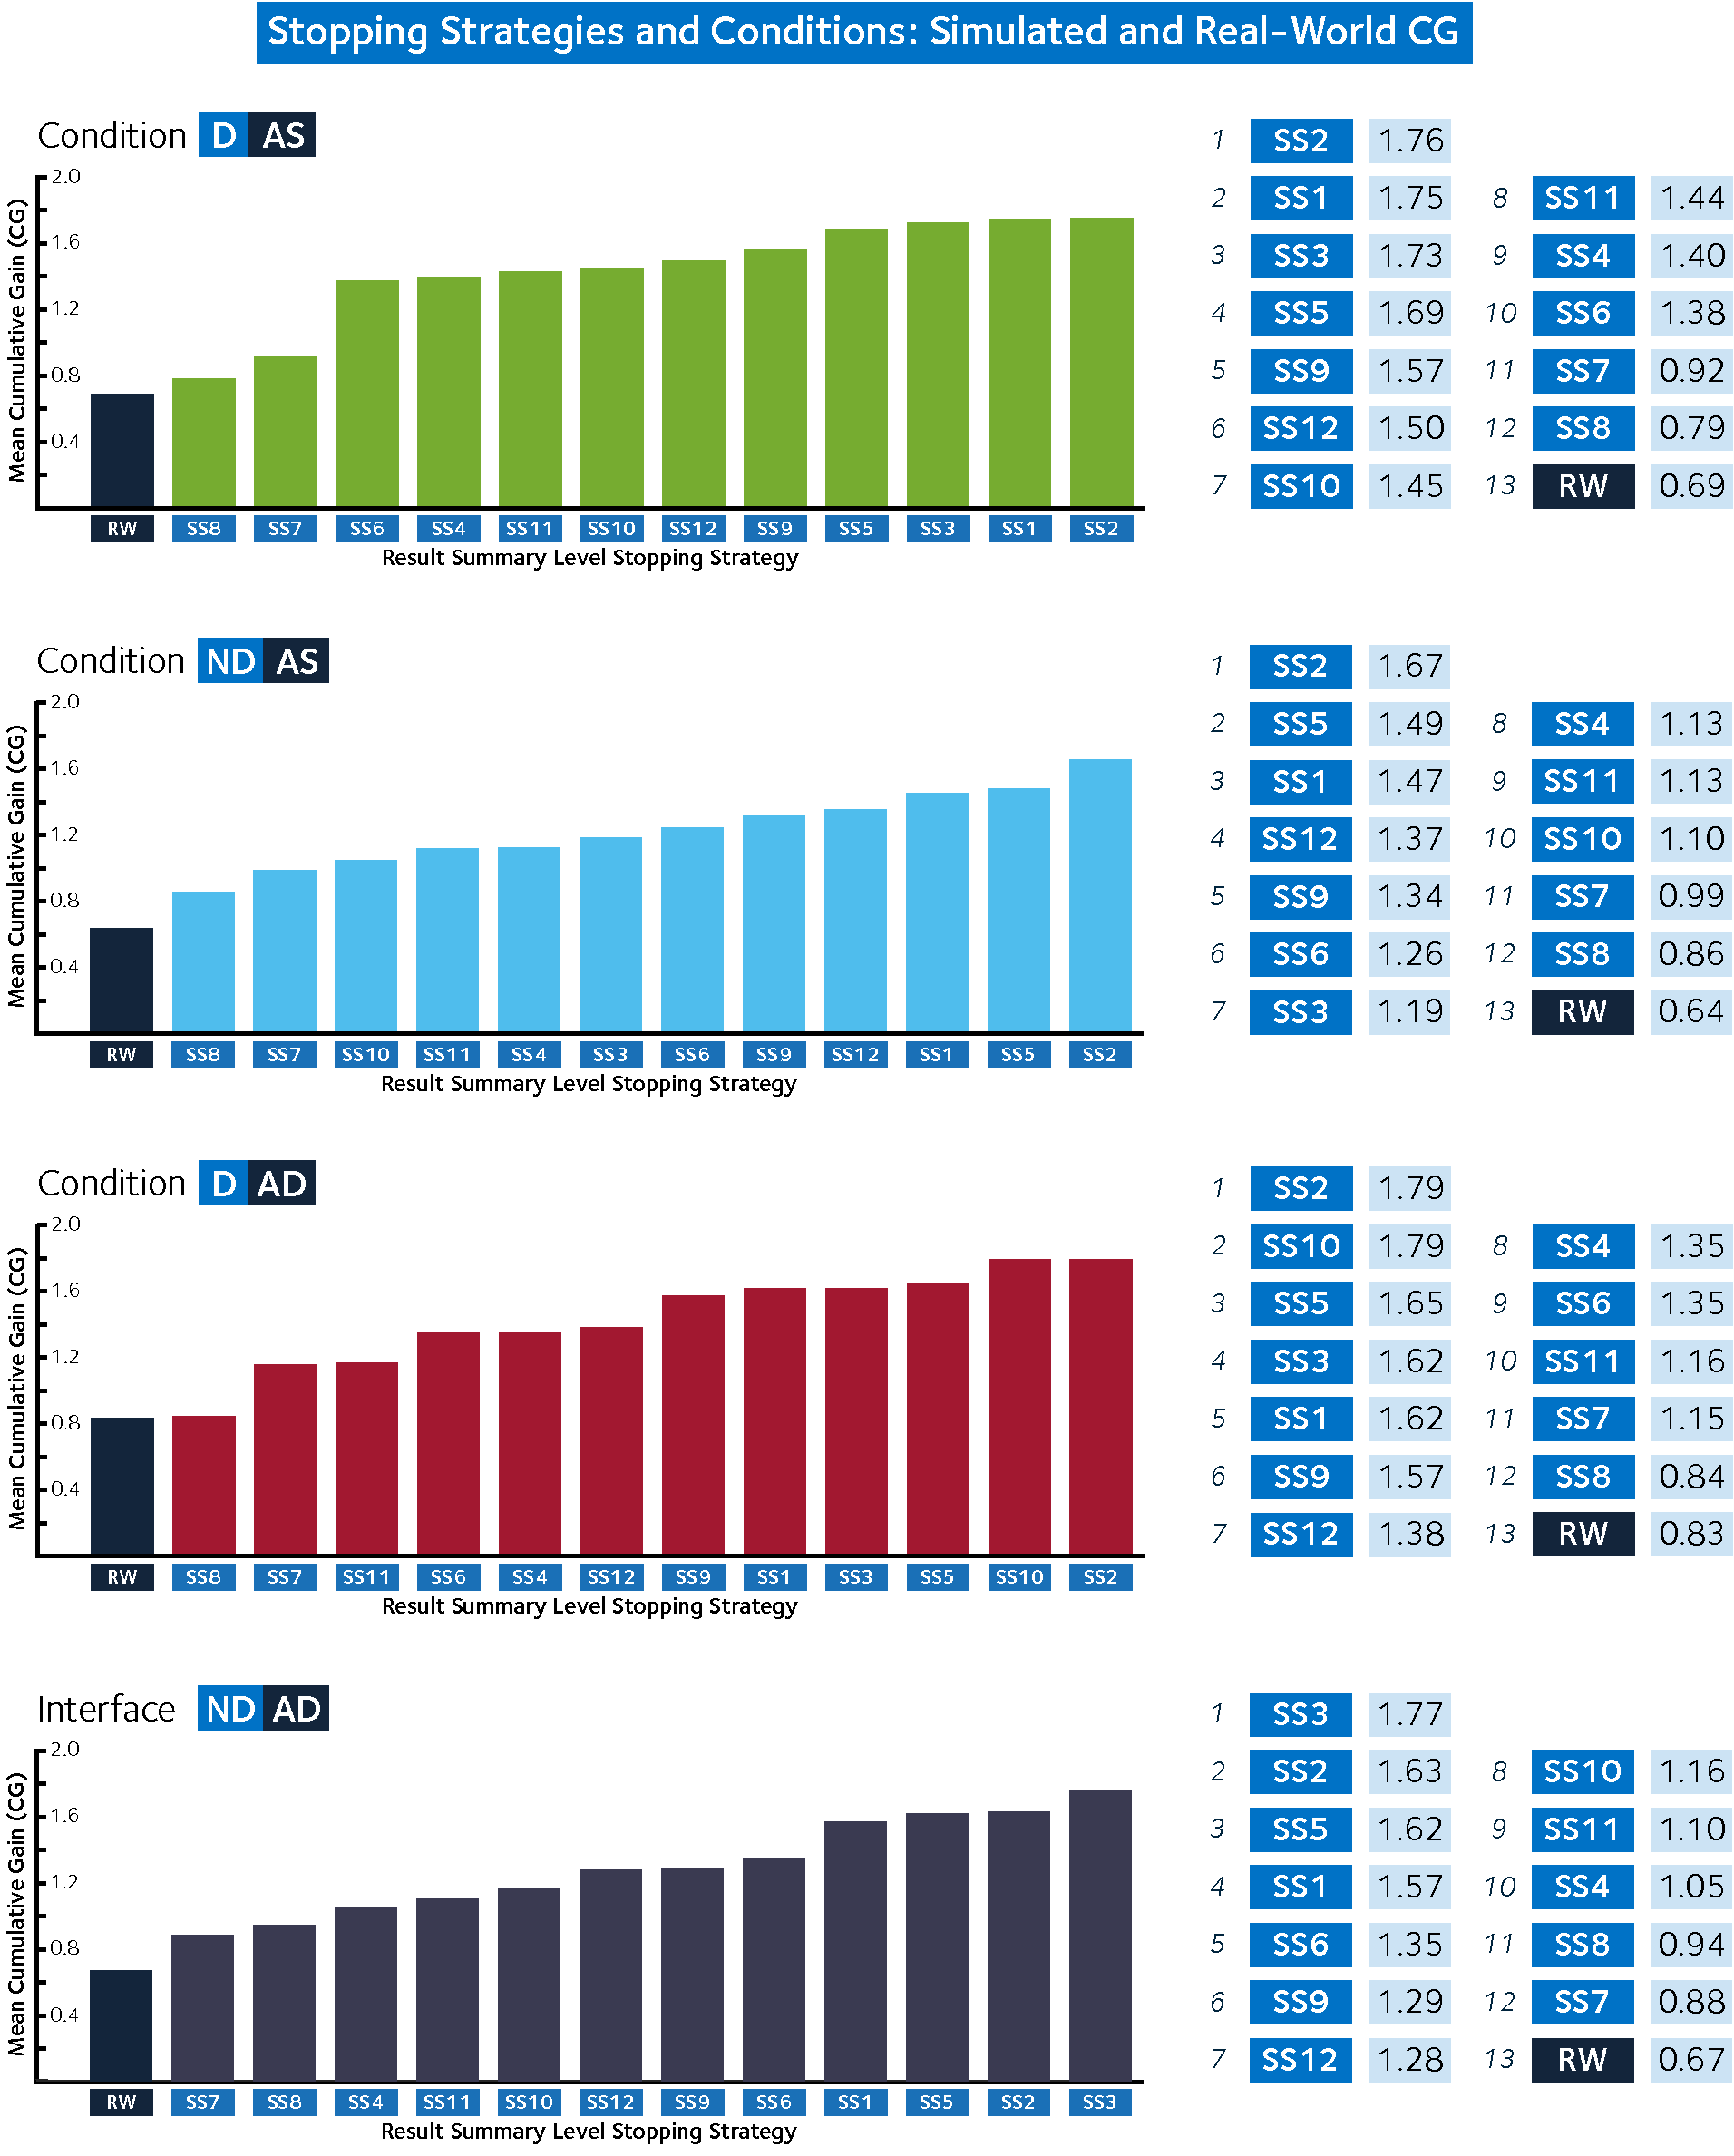
\includegraphics{figures/ch8-comparison_rankings.pdf}}
    \caption[Comparison~\gls{acr:cg} rankings (diversification)]{Bar charts, one per experimental condition, demonstrating the mean level of~\gls{acr:cg} attained by each result summary level stopping strategy. Ordered by~\gls{acr:cg}, these values are reached using the threshold configurations yielding the best approximations to actual searcher behaviour, as shown in Table~\ref{tbl:ch8_sim_comp}. Also included are the mean real-world searcher~\gls{acr:cg} values for each interface.}
    \label{fig:ch7_sim_comparison_rankings}
\end{figure}

For conditions \dualbluebox{D}{AS} and \dualbluebox{D}{AD}, we find that stopping strategy \blueboxbold{SS10-RELTIME} also yields the highest level of~\gls{acr:cg} after the real-world means. This is in contrast to stopping strategy \blueboxbold{SS1-FIX} that yielded the lowest MSE (approximating mean click depths) for these conditions. For condition \dualbluebox{ND}{AD}, frustration-based stopping strategy \blueboxbold{SS2-NT} was the stopping strategy offering the best~\gls{acr:cg} ($2.73$), along with \blueboxbold{SS3-NC} that offered the highest overall~\gls{acr:cg} for condition \dualbluebox{D}{AS}, as previously mentioned. This means that instead of following their actual behaviours, the real-world searchers would have on average attained a slightly higher level of~\gls{acr:cg} if they rigidly followed \dualbluebox{SS3-NC}{@9}. However, the difference is not significant.

Looking towards the lower end of the bar charts in Figure~\ref{fig:ch7_sim_comparison_rankings}, we note that stopping strategies \blueboxbold{SS6-DT}, \blueboxbold{SS7-DKL}, \blueboxbold{SS8-IFT} and \blueboxbold{SS12-RBP} frequently appear at these lower rankings. In particular, \blueboxbold{SS12-RBP} consistently ranks last, with the lowest level of~\gls{acr:cg} attained. For this stopping strategy, we can see the plot in Figure~\ref{fig:ch8_sim_comparison_plots} demonstrates that it underestimates the stopping depths, with searchers stopping at much lower mean depths per query. These values, being much lower than the mean real world equivalents, result in higher MSE values. Underestimation can also be clearly seen for \blueboxbold{SS6-DT}, with the lowest MSE values attained in the range of $7.10$ to $9.97$ across the four experimental interfaces. The same can be observed for \blueboxbold{SS7-DKL}, with variable lines and no smooth curve present. Contrast this plot for example to that of \blueboxbold{SS4-SAT}, with a smooth curve and the lowest point of each line close to the real-world means. Again, these findings are discussed in more detail in Chapter~\ref{chap:conclusions}.

\section{Chapter Summary}
In this chapter, we have examined how varying search task types and goals affect the behaviour, performance and user experience of searchers. This was conducted via a crowdsourced user study, as reported in Section~\ref{sec:diversity:users}. From this user study, we then subsequently used interaction data to ground an extensive set of simulations of interaction, reported in Section~\ref{sec:diversity:simulated}. These simulations were used to determine how each of the twelve stopping strategies proposed in Chapter~\ref{chap:strategies} performed and approximated the mean stopping behaviours of searchers. In turn, these findings provide answers to our two high-level research questions \darkblueboxbold{HL-RQ3a} and \darkblueboxbold{HL-RQ3b}, when tasks and goals are varied.

Considering the user study first, we trialled four different experimental conditions. These were \dualbluebox{D}{AS} \emph{(diversified system, aspectual task),} \dualbluebox{ND}{AS} \emph{(non-diversified system, aspectual task),} \dualbluebox{D}{AD} \emph{(diversified system, ad-hoc task)} and \dualbluebox{ND}{AD} \emph{(non-diversified system, ad-hoc task).} Under system \blueboxbold{ND}, results were returned with the standard BM25 retrieval model ($\beta=0.75$). However, for system \blueboxbold{D}, results were re-ranked according to a diversification algorithm, ensuring that a more diverse set of results for the given topic were returned. Considering tasks, searchers were either asked to save four relevant documents (for task \darkblueboxbold{AD}), or save four relevant documents that contained at least one new aspect of the topic being examined (for task \darkblueboxbold{AS}).

While significant differences existed between the performance of systems \blueboxbold{ND} and \blueboxbold{D}, no significant differences were observed when considering searcher behaviours, although notable trends were observed. Subjects when using system \blueboxbold{D} did perform better on average, saving more~\gls{acr:trec} relevant documents, and~\gls{acr:trec} relevant documents with at least one new entity. Evidence was also found to support our~\gls{acr:ift}-based hypotheses. However, the lack of significant differences between the experimental conditions showed that bigger differences were required before individuals would have been able to subjectively begin to report on whether the two systems yielded a different experiment.

From the user study, we then took the interaction data to derive a series of interaction probabilities and costs. In turn, these were used to ground an extensive set of simulations of interaction. Split across performance (addressing \darkblueboxbold{HL-RQ3a}) and comparison runs (addressing \darkblueboxbold{HL-RQ3b}), we examined each individual stopping strategy in both terms of overall performance, and how well they approximated actual searcher stopping behaviours. These were run across each of the four experimental conditions. Findings for \darkblueboxbold{HL-RQ3a} show that all twelve stopping strategies offered reasonable levels of~\gls{acr:cg}. We found that stopping strategies \blueboxbold{SS1-FIX} and \blueboxbold{SS5-COMB} offered the best levels of~\gls{acr:cg} (with \blueboxbold{SS1-FIX} performing best under condition \dualbluebox{ND}{AD}). Only stopping strategy \blueboxbold{SS8-IFT} consistently yielded significantly poorer performance than the best performing strategies, perhaps due to how the strategy was instantiated.

When considering \darkblueboxbold{HL-RQ3b}, we found that under system \blueboxbold{D}, \blueboxbold{SS1-FIX} offered the best approximations to searcher behaviours, with \blueboxbold{SS10-RELTIME} providing the best approximations for system \blueboxbold{ND}. This is an interesting result -- and perhaps pertains to the fact that system \blueboxbold{D} offered better performance on average than system \blueboxbold{ND}. However, when comparing the simulation results to the real-world means, we found that the simulated counterparts of the real-world subjects 

Along with the findings obtained from Chapter~\ref{chap:snippets}, these findings will be discussed in detail in Chapter~\ref{chap:conclusions}. The following chapter shifts from an examination of result summary level stopping to the new stopping decision point --~\gls{acr:serp} level stopping. \emph{If included, does a simulated searcher employing~\gls{acr:serp} level stopping yield better overall performance and approximations of real-world stopping behaviours?}
